\chapter{Unitarizable highest weight modules}

One of the main open problem of representation theory is classification of unitary modules of Lie groups. Apart from the finite-dimensional representations (which are unitary for compact Lie groups) one of the classes of modules where a complete classification was obtained is the class of unitarizable modules of highest weight. It is precisely the intersection of BGG category $\mathcal{O}$ and Harish-Chandra $(\mathfrak{g}, K)$-modules. It was proved already by Harish-Chandra that these modules can occur only in the hermitian symmetric case, see \cite{harish-chandra_representations_1955}, \cite{harish-chandra_representations_1956-1} and \cite{harish-chandra_representations_1956} for details.

A sufficient and necessary condition for unitarizability of a highest weight module appears in \cite{garland_unitarizable_1981}. Independently, these modules were classified by Jakobsen in \cite{jakobsen_last_1981}, \cite{jakobsen_hermitian_1983} with later development in \cite{jakobsen_intrinsic_1996}. Another, yet independent approach, was given by \cite{enright_classification_1983} with later simplification in \cite{joseph_annihilators_1992}. In \cite{adams_unitary_1987} it was shown that all unitarizable highest weight modules can be obtained via the derived functor construction from either a one-dimensional or a unipotent representation. This  parameterization given here fits in nicely with the Langlands classification and the coadjoint orbit picture.  

In this chapter we follow mainly the article \cite{enright_classification_1983} and reorganization of the unitarizable weight into integral cones that was presented in \cite{davidson_differential_1991}. 

\section{Classification}

The algebra $\lie{k}$ has a one-dimensional center which is complementary to the span of $\roots_c$. We pick a generator $\zeta$ of the center by requiring $\frac{2 \langle \zeta,\beta \rangle}{\langle \beta, \beta \rangle} = 1$, where $\beta$ is the unique maximal noncompact root\footnote{Equivalently, $\beta$ is the highest weight of $\lie{k}$-representation $\lie{p}_+$.} of $\roots^+$. Now any line $\lambda+z\zeta$ for $z\in\C$ can be uniquely written as $\lambda_0 + z\zeta$ with
\[
 \langle \lambda_0 + \rho,\beta \rangle = 0, \quad \rho =\sum_{\alpha\in\roots^+} \alpha.
\]

If $L(\lambda)$ is an irreducible unitarizable module for $\lambda=\lambda_0+z\zeta$, then $z$ must be real and the $K_\C$-finiteness implies that $\lambda$ must be $\roots^+_c$-dominant integral. Write the generalized Verma module $M(\lambda)$ as $S(\lie{p}_+)\otimes F(\lambda_0) \otimes \C_z\zeta$. If we fix a basis of $\lie{g}$ and $F(\lambda_0)$, we may view the modules $M(\lambda)$ as defined on the same vector space $S(\lie{p}_+)\otimes F(\lambda_0)$ where the action of $\lie{g}$ is given by polynomial expressions in $z$. Likewise, we may view the Shapovalov form on $M(\lambda)$ as a bilinear form on $S(\lie{p}_+\otimes F(\lambda_0)$ with values in complex polynomials $\C[z]$.

A $\lie{g}$-module $M$ is called unitarizable if there exists (necessarily unique up to a multiple) positive definite contravariant form on $M$. The preceding paragraph explains the structure of the set of $z\in\R$ such that the module $M(\lambda)$ is unitarizable.

\begin{figure}[H]\label{fig:struct}
  \begin{center}
  \begin{tikzpicture}
      \node[croot] at (2,0) [label=above:$A(\lambda_0)$] {};
      \node[croot] at (3,0) {};
      \node[croot] at (6,0) [label=above:$B(\lambda_0)$] {};
      \draw[thick] (0,0) to (2,0);
      \draw [dotted] (4,0) to (5,0);
      \draw[<->] (2,-0.5) -- (3,-0.5);
      \node at (2.5,-0.5) [label=below:$C$] {};
  \end{tikzpicture}
  \end{center}\caption{Structure of unitarizable weights} %TODO dodelat mark na 0
\end{figure}

\begin{theorem}[Theorem 2.4 of \cite{enright_classification_1983}]
 The set of real numbers $z$ with $L(\lambda_0 + z\zeta)$ a unitarizable $\lie{g}$-module is given by the set
\[
  \{z \in \mathbb{R}\, |\, z \leq A(\lambda_0)\} \cup \{ z=A(\lambda_0) + k C(\lambda_0)\,|\, z \leq B(\lambda_0) \et k\in \mathbb{N}_0\},
\]
where $A(\lambda_0)$, $B(\lambda_0)$ and $C(\lambda_0)$ are real numbers expressible in terms of certain root systems $Q(\lambda_0)$ and $R(\lambda_0)$ associated to $\lambda_0$. Moreover $C(\lambda_0)$ is independent of $\lambda_0$ and depends only on the type of $\lie{g}_0$. The values of $C$ are listed in Table \ref{tbl:C} and the structure of the set of unitarizable highest weights is depicted in Figure \ref{fig:struct}.
	
The discrete series representation corresponds to $z <0$ and limit of discrete series representation corresponds to $z=0$. For $z  < A(\lambda_0)$ we have $L(\lambda) = M(\lambda)$ (i.e. the generalized Verma modules are irreducible) and for all $z \geq A(\lambda_0)$ such that $L(\lambda)$ are unitarizable the generalized Verma modules are reducible.%, hence the elements of  $\{z=A(\lambda_0) + kC| \, z \leq B(\lambda_0) \et k\in \mathbb{N}_0 \}$ are called  reduction points or points of reducibility.

\begin{table}[h]\label{tbl:C}
\[\begin{array}{c|ccccccc}
\lie{g}_0 & \mathrm{SU}(p,q) & \mathrm{Sp}(n,\mathbb{R}) & \mathrm{SO}^*(2n) & \mathrm{SO}(2,2n-2) & \mathrm{SO}(2,2n-1) & \mathrm{E}_6 & \mathrm{E}_7\\\hline
C & 1 & \frac{1}{2} & 2 & n-2 & n-\frac{3}{2} & 3 & 4
\end{array}\]\caption{Distance between points of reducibility}
\end{table}
\end{theorem}

Let $\roots_c(\lambda_0) := \{ \alpha \in \roots_c | \langle \alpha,\lambda_0 \rangle = 0 \}$ and recall the definition of $\beta$ the maximal non-compact root. Take the root subsystem of $\roots$ generated by $\pm \beta$ and $\roots_c(\lambda_0)$ and decompose it into a disjoint union of simple root systems. Let $Q(\lambda_0)$ be the root system in this union which contains $\beta$.

If $\roots$ has two root lengths and if there are short compact roots $\alpha$ not orthogonal to $Q(\lambda_0)$ with $\frac{2 \langle \lambda_0,\alpha \rangle}{\langle \alpha, \alpha \rangle}  =1$, then let $\Psi$ be the root system generated by $\pm \beta, \roots_c(\lambda_0)$ and all such $\alpha$. Let $R(\lambda_0)$ be the simple component of $\Psi$ which contains $\beta$. If $\roots$ has only one root lenght or if no such $\alpha$ exists, then put $R(\lambda_0) = Q(\lambda_0)$.

Since these root systems are subsystems of $\roots$ and since each has compact and noncompact roots, each is a root system of a Hermitian symmetric pair.

There is a convenient way to construct $Q(\lambda_0)$ by means of Dynkin diagrams. Draw a Dynkin diagram of $\lie{g}$ and delete the unique node corresponding to simple noncompact root. Now adjoin to the resulting diagram $-\beta$ by the usual rules as when constructing extended Dynkin diagrams. The maximal connected subdiagram containing $-\beta$ such that its every compact simple root is orthogonal to $\lambda_0$ is the Dynkin diagram of $Q(\lambda_0)$. We illustrate on the case of $\lie{su}(p,q)$. Here the noncompact root $\beta$ is $\alpha_p$ and we get the following extended Dynkin diagram.
\begin{figure}[H]\label{fig:Q}
  \begin{center}
     \begin{tikzpicture} % SU(p,q) ~ A_{n-1} relative
	\node[croot] (a1) [label=below:$\alpha_1$] {};
	\node[croot] (a2) [right= of a1] [label=below:$\alpha_2$] {};
	\node[croot] (a3) [right= of a2] [label=below:$\alpha_3$] {};
	\node (a4) [right= of a3] {};
	\node[nroot] (a5) [above right=of a4] [label=above:$-\beta$] {};
	\node (a6) [below right=of a5] {};
	\node[croot] (a7) [right=of a6] [label=below:$\alpha_{n-3}$] {};
	\node[croot] (a8) [right=of a7] [label=below:$\alpha_{n-2}$] {};
	\node[croot] (a9) [right=of a8] [label=below:$\alpha_{n-1}$] {};
	\draw (a1) to (a2) to (a3); \draw [dotted] (a3) to (a4);
	\draw [dotted](a6) to (a7);
	\draw (a7) to (a8) to (a9);
	\draw (a1) to (a5) to (a9);
     \end{tikzpicture}
  \end{center}\caption{The Dynkin diagram of $Q(\lambda_0)$} 
\end{figure}
If we write with respect to the basis of fundamental weights $\lambda_0 = \sum_i a_i \omega_i$ we see that $Q(\lambda_0)$ is a root system of $\lie{su}(p',q')$ where $p'$ and $q'$ are maximal such that the coefficients $a_1,a_2,\ldots,a_{p'}$ and $a_{n-q'+1},a_{n-q'+2}, \ldots, a_n$ are nonzero.

The root system $R(\lambda_0)$ is different from $Q(\lambda_0)$ only in two cases. The first one is $\lie{g}_0=\lie{sp}(n,\R)$ where $Q(\lambda_0) = \lie{sp}(n',\R)$ and $R(\lambda_0) = \lie{sp}(n'',\R)$ with $n' < n'' \leq n$. The second one is $\lie{g}_0=\lie{so}(2,2n-1)$ where $Q(\lambda_0) = \lie{su}(1,n-1)$ and $R(\lambda_0) = \lie{so}(2,2n-1)$ with $\lambda_0 = (\lambda_1,\frac{1}{2},\ldots,\frac{1}{2})$ in the $\epsilon$-basis.

The following two theorems finish the general classification of unitarizable highest weight modules.

\begin{theorem}[Theorem 2.8 of \cite{enright_classification_1983}]
 Let $\roots^+_{c,1} := \roots^+_c \cap Q(\lambda_0)$ and let $\roots^+_{c,2} := \roots^+_c \cap R(\lambda_0)$. Denote by $\rho_{c,i}$ half of the sum of roots in $\roots^+_{c,i}$.
 
 If $\lie{g}_0=\lie{so}(2,2n-1)$ and $Q(\lambda_0) \neq R(\lambda_0)$ then \[B(\lambda_0) = 1 + \frac{\langle \rho_{c,2},\beta\rangle}{\langle \beta, \beta \rangle}.\]
 In all other cases \[B(\lambda_0) = 1 + \frac{ \langle \rho_{c,1} + \rho_{c,2} , \beta \rangle}{\langle \beta, \beta \rangle}.\]
\end{theorem}


\begin{theorem}[Theorem 2.10 of \cite{enright_classification_1983}]\label{thm:reduction_points}
 The first reduction point $A(\lambda_0)$ is given by\footnote{Or in other words: The number of reduction points equals the split rank of $Q(\lambda_0)$.}
 \[
   A(\lambda_0) = B(\lambda_0) - (\text{split rank } Q(\lambda_0) -1) C.
 \]
\end{theorem}

Now let's see what we can tell about the maximal module $J(\lambda)$ of the generalized Verma module $M(\lambda)$. %The following was proved in \cite{davidson_differential_1991}.

\begin{theorem}[Theorem 3.1 of \cite{davidson_differential_1991}]
 Suppose $L(\lambda) = M(\lambda)/J(\lambda)$ is unitarizable and $J(\lambda)\neq 0$. Then
 \begin{enumerate}
  \item $H^1(\lie{p}_-,L(\lambda))$ is an irreducible $\lie{k}$-module
  \item $J(\lambda)$ is generated over $S(\lie{p}_+)$ by an irreducible $\lie{k}$-submodule $J(\lambda)^0$ isomorphic to $H^1(\lie{p}_-,L(\lambda))$.
 \end{enumerate}
\end{theorem}


%Let $J(\lambda)$ denote the maximal submodule of the generalized Verma module $M(\lambda)$. For all unitarizable highest weight modules we have  $J(\lambda)$  generated by $\lie{U(g)}$ from an irreducible $\lie{k}$-module.
In particular, the generator of $J(\lambda)$ must be contained in some component $S^k(\lie{p}_+)\otimes F(\lambda)$. This $k$ is called \emph{level of reduction} of $L(\lambda)$ and is denoted by $l(\lambda)$.

\begin{definition}
 The set of reduction points $\Lambda_r$ is the union of all reduction points. Explicitly
 \[
 \Lambda_r := \{ \lambda = z\zeta + \lambda_0 \in \lie{h}^* | z = A(\lambda_0) +kC, k\in\N_0, z \leq B(\lambda_0) \}.
 \]

 For $\lambda \in \Lambda_r$ let $a(\lambda) := (Q(\lambda_0),R(\lambda_0),l(\lambda))$ and let $\mathcal{A}$ denote the set of all such triples as $\lambda$ ranges over $\Lambda_r$. For $a\in\mathcal{A}$, let $\Lambda_a$ denote the set of all $\lambda\in\Lambda_r$ with $a(\lambda)=a$.
\end{definition}

Now we can look more closely at the structure of the set of reduction points. 

\begin{corollary}[of \ref{thm:reduction_points}]
 Let $a=(Q,R,l)\in\mathcal{A}$ and let $\lambda\in\Lambda_a$. If we write $\lambda= z\zeta + \lambda_0$, then $z=B(\lambda)-(l-1)C$ and on the other hand for $\lambda=(B - nC)\zeta + \lambda_0 \in \Lambda_r$ we have $l(\lambda) =n+1$.
\end{corollary}

Let $\lie{h}^*_\R$ denote the real span of the roots. A \emph{cone} with vertex zero (in $\lie{h}^*_\R$) is the intersection of a (nonempty) collection of closed half spaces. Each cone $C$ is thus determined by a finite set $\{h_i \in \lie{h}|i=1,\ldots,k\}$ with $C= \{ \lambda \in \lie{h}^*_\R | \lambda(h_i) \geq 0, i=1,\ldots k\}$. An \emph{integral cone} will be the intersection of a cone with the set of all $\lie{k}$-integral points of $\lie{h}^*.$ For an integral element $\nu\in\lie{h}^*$, a translated cone with vertex $\nu$ is a set of the form $\nu + C$ with $C$ some integral cone.

\begin{definition}
 For $a=(Q,R,l)\in\mathcal{A}$, let $C_a$ be the integral cone of $\lie{k}$-dominant integral elements in $\lie{h}^*_\R$ which are orthogonal to elements in $R$.
\end{definition}

%Since the root system $R$ always contains $\beta$, the representations $L(\lambda)$ are in fact finite-dimensional for $\lambda\in C_a$.

For concrete calculations the following lemma can be useful. 

\begin{lemma}[Section 4.3 of \cite{enright_resolutions_2004}]
The cone $C_{Q, R, l}$ consists of positive integral multiples of weights of the form $\omega_i - (\omega_i, \beta^\vee) \zeta,$ where $\omega_i$ is a fundamental weight corresponding to simple root $\alpha_i$ that does not belong to $R$.
\end{lemma}
\begin{proof}
 Any  $\lie{k}$-dominant integral weight can be written in the form $\mu = \sum_i a_i \omega_i + b \zeta,$ where $a_i$ are nonnegative integers. Such a weight is perpendicular to $R$ if and only if it is perpendicular to all compact simple roots contained in $R$ and to the noncompact root $-\beta$, i.e. to the simple roots of the root system $R$. The crucial observation here is that for each Hermitian symmetric space the weight $\zeta$ is in fact the fundamental weight corresponding to the simple noncompact root. Hence we have 
\[
0 = \left(\sum a_i \omega_i + b \zeta, \alpha_i^\vee \right) = a_i 
\] 
for all compact simple roots of  $R$ and 
\[
0 = \left(\sum a_i \omega_i + b \zeta, \beta^\vee \right)
\]
for the noncompact root. Recalling the definition of $\zeta$ and solving for $b$ we see that the cone consists of vectors of the form $\sum a_i (\omega_i - (\omega_i, \alpha_i^\vee)\zeta)$ where the sum is only indices whose simple roots are not in $R$.
\end{proof}

\begin{proposition}[Proposition 6.6 of \cite{davidson_differential_1991}]
 The set of reduction points $\Lambda_r$ is the disjoint union of the sets $\Lambda_a, a\in\mathcal{A}$.

 Each set $\Lambda_a$ is a translated integral cone with vertex $\lambda_a + C_a$. We list the vertices $\lambda_a$ in sections \ref{sec:su} through \ref{sec:exceptional}.
\end{proposition}
\begin{proof}
 The first statement is trivial and the second one follows by case by case computations.
\end{proof}

The next proposition gives an alternative way to compute the highest weight of the maximal submodule.

\begin{proposition}[Proposition 6.8 of \cite{davidson_differential_1991}]
 Suppose $\lambda\in\Lambda_a$ with $a=(Q,R,l)$. Let $u$ and $v$ denote respectively the unique elements of maximal length in the Weyl groups for the positive root systems $Q\cap \roots^+_c$ and $R\cap \roots^+_c$ and let $\mu$ denote the highest weight of the maximal submodule $J(\lambda)$. Then
 \[
  \mu = \lambda + \frac{1}{2}(u \mu_l + v \mu_l)
 \]
 in all cases except when $\lie{g}_0=\lie{so}(2,2n-1)$ and $Q\neq R$. In this case
 \[
  \mu = \lambda + \frac{1}{2}(\mu_l + v\mu_l).
 \]

 Moreover, in all cases $F(\mu)$ occurs with multiplicity one in $M(\lambda+\rho)$ and in all cases $F(\mu)$ is a PRV component of a tensor product in $S(\lie{p}_+)\otimes F(\lambda)$.
\end{proposition}

The next theorem  deals with effect of a sort of `translation functor' on unitarizable highest weight modules.
\begin{theorem}[Factorization theorem 6.15 of \cite{davidson_differential_1991}]
 Fix $a\in\mathcal{A}$ and let $\lambda = \lambda_a + \lambda'\in\Lambda_a$. Let $J(\lambda)^0$ and $J(\lambda_a)^0$ be the $\lie{k}$-modules that generate $J(\lambda)$ and $J(\lambda_a)$. Extend the $\lie{k}$-equivariant projection \[P:F(\lambda_a)\otimes F(\lambda') \to F(\lambda)\] to a mapping $\widetilde{P}:M(\lambda_a) \otimes F(\lambda') \to M(\lambda)$ by \[\widetilde{P}(F\otimes v) (T) := P(F(T)\otimes v),\]
  where we have used that $M(\lambda_a) = S(\lie{p}_+)\otimes F(\lambda_a)$.

Let $\mu$ and $\mu_a$ denote the highest weights of  $J(\lambda)^0$ and $J(\lambda_a)^0$. Then
 \begin{enumerate}
  \item $\mu  = \mu_a+\lambda'$
  \item $P(J(\lambda_a)^0\otimes F(\lambda')) = J(\lambda)^0$ and 
  \item $P(J(\lambda_a)\otimes F(\lambda')) = J(\lambda)$.
 \end{enumerate}
\end{theorem}

\section{Nilpotent cohomology of unitarizable highest weight modules}

The convention employed in this section is that we omit the terms whose indices are outside natural boundaries. 

\begin{definition}\label{def:cohomology_roots}
Let $\Psi_\lambda$ be the set if roots in $\roots$ which are orthogonal to $\lambda+\rho$ and let $\Psi_\lambda^+ = \Psi_\lambda \cap \roots^+$. Denote by $\roots_{n,\lambda}^+$ the roots which satisfy the following condititions
 \begin{enumerate}
    \item $\alpha \in \roots_n^+$ and $(\lambda+\rho,\alpha^\vee)$ is a positive integer;
    \item $\alpha$ is orthogonal to $\Psi_\lambda$;
    \item $\alpha$ is short if there exist a long root in $\Psi_\lambda$.
 \end{enumerate}
 
 Let $W_\lambda$ be the subgroup of $W$ which is generated by reflections $s_\alpha$ for $\alpha\in \roots_{n,\lambda}^+$.
 
 Let $\roots_\lambda$ be the subset of $\roots$ of elements $\beta$ with $s_\beta\in W_\lambda$ and let $\roots_{\lambda,c} = \roots_c \cap \roots_\lambda$, $\roots_{\lambda,c}^+ = \roots_{\lambda,c} \cap \roots^+$.
 
 Finally, define  $W^{c,i}_\lambda = \{ w \in W_\lambda | w \rho \text{ is } \roots^+_{\lambda, c}\text{-dominant and } l_\lambda(w)=i \}$.
\end{definition}


\begin{theorem}[3.7 \cite{davidson_differential_1991}]\label{thm:cohomology}
 Let $L$ be unitarizable with highest weight $\lambda $. Then for $i\in \mathbb{N}$ we have
\begin{equation}\label{eq:cohomology}
 H^i(\lie{p}_+,L)\simeq \bigoplus_{w\in W^{c,i}_\lambda} F(\overline{w(\lambda+\rho)} - \rho)
\end{equation}
where  $\overline{\lambda}$ is the unique $\roots_c^+$-dominant element in the $W_c$ orbit of $\lambda$.
\end{theorem}

\begin{remark}
 The $\lie{k}$-weight of the first cohomology is given by $\lambda_0-\rho$ where $\lambda_0$ is the unique $\roots_c^+$ dominant element in the $W_c$ orbit of $s_{\gamma_0}\lambda$ for the unique noncompact simple root $\gamma_0 \in \roots_\lambda^+$.
\end{remark}

\begin{lemma}\label{lem:singular_are_noncompact}
 Let $\lambda$ be a highest weight of a unitarizable highest weight module. If a positive root is orthogonal to $\lambda + \rho$ then it must be noncompact.
 \[
  \alpha \in \roots^+: \alpha \perp \lambda + \rho \Longrightarrow \alpha \in \roots^+_n
 \]
\end{lemma}
\begin{proof}
 Every positive roots can be written as a positive linear combination of simple roots, i.e. $\alpha = \sum_i c_i \alpha_i$ where $c_i \geq 0$. The fundamental weights form a basis of $\lie{h}^*$ and thus $\lambda = \sum_i k_i \omega_i$. Now we just use the defining property of fundamental weights $\frac{2(\alpha_i,\omega_j)}{(\alpha_i,\alpha_i)} = \delta_{ij}$ to compute
 \begin{align*}
  (\alpha,\lambda+\rho) & = \sum_{i,j} \left(  c_i k_j (\alpha_i,\omega_j) + c_i (\alpha_i,\omega_j) \right ) \\
			& = \sum_{i,j} \left( c_i k_j \frac{(\alpha_i,\alpha_i)}{2} \delta_{ij} + c_i \frac{(\alpha_i,\alpha_i)}{2} \delta_{ij} \right ) \\
			& = \sum_i c_i \frac{(\alpha_i,\alpha_i)}{2} (k_i + 1).
 \end{align*}
 If $\lambda$ is a highest weight of a unitarizable module, then all but one of the coefficients $k_i$ are nonnegative and the only possibly negative coefficient corresponds to the fundamental weight dual to the coroot of the unique noncompact simple root - let's denote it's index by $i_0$. If the scalar product $(\alpha, \lambda+\rho)$ is zero, then $c_{i_0}$ must be nonzero -- all the remaining terms in the sum are nonnegative. But $c_{i_0} \neq 0$ is equivalent to $\alpha$ being noncompact.
\end{proof}


\begin{example} 
 Let us take $\lie{g} = \lie{so}(2,2n-2)$ with $\lambda = (2-n)\omega_1$. Then in the epsilon basis we have $\lambda + \rho = (1,n-2,\ldots,1,0)$ and $\Psi_\lambda^+ = \{ \epsilon_1 - \epsilon_{n-1}\}$. The only noncompact root that is orthogonal to $\epsilon_1 -  \epsilon_{n-1}$ and whose scalar product with $\lambda + \rho$ is positive integral is $\alpha = \epsilon_1 + \epsilon_{n-1}$. Thus we get $\roots_{n,\lambda}^+ = \epsilon_1 + \epsilon_{n-1} = \roots_\lambda$. It follows that
\begin{align*}
 H^0(\lie{p}_-,L((2-n)\omega_1)) &= F((2-n)\omega_1)\\
 H^1(\lie{p}_-,L((2-n)\omega_1)) &= F(-n\omega_1)\\
 H^i(\lie{p}_-,L((2-n)\omega_1)) &= 0 \text{ for } i\geq 2.
\end{align*} 

Similarly there is only one root generating $W_\lambda$ for $\lie{g} = \lie{so}(2,2n-1)$ and $\lambda = (\frac{3}{2} - n)\omega_1$ and we get that in that case
\begin{align*}
 H^0(\lie{p}_-,L((\frac{3}{2}-n)\omega_1)) &= F((\frac{3}{2}-n)\omega_1)\\
 H^1(\lie{p}_-,L((\frac{3}{2}-n)\omega_1)) &= F((-\frac{1}{2}-n)\omega_1)\\
 H^i(\lie{p}_-,L((\frac{3}{2}-n)\omega_1)) &= 0 \text{ for } i\geq 2.
\end{align*}

Moreover, by inspecting the tables \ref{tbl:so_even} and \ref{tbl:so_odd}, we see that in both of these cases the cone $C_a$ is empty.
\end{example}

\begin{remark}
 The formula \eqref{eq:cohomology} is actually stated a little bit differently in \cite{enright_analogues_1988}. Namely, the finite dimensional modules appearing in the cohomology are $F(\overline{w}\cdot lambda)$ where $\overline{w}$ is the minimal length representant of $w$. The same formula appears in a recent article \cite{enright_diagrams_2014}. However, this formula is wrong as the following example shows.

Consider $\lie{su}(1,2)$ and weight $\lambda = -(a+2)\omega_1 + (a+1)\omega_2$. The reduced hermitian pair is of type $A_1$ and it's given by $\{\epsilon_1 - \epsilon_3 \}$. The associated reflection is $s_{\epsilon_1 - \epsilon_3} = s_1 s_2 s_1$ and its minimal coset representative is $s_1 s_2$. It's affine action on $\lambda$ gives $-2\omega_1 - (a+2)\omega_2$ which is not $\roots_c^+$-dominant. On the other hand the (normal) action of $s_1 s_2 s_1$ on $\lambda + \rho$ gives $ -(a+2)\omega_1 + (a+1)\omega_2$ which is $\roots_c^+$-dominant and hence the first cohomology is $F(-(a+3)\omega_1 + a\omega_2).$
\end{remark}

Cohomologies of all unitarizable modules for the two expceptional types are explicitely computed in \cite{enright_resolutions_2004-1}. The papers \cite{enright_hilbert_2004}, \cite{enright_resolutions_2004} treat also certain weights for the classical types $\lie{su}(p,q)$, $\lie{sp}(n,\R)$ and $\lie{so}^*(2n).$  The orthogonal cases $\lie{so}(2,2n-2)$, $\lie{so}(2,2n-1)$ are rather easy and are calculated completely in sections \ref{sec:conf_even} and \ref{sec:conf_odd}. For the other classical types we calculate some of the data that go into the formula \eqref{eq:cohomology} and calculate the cohomologies completely in small ranks in appendix \ref{app:cohomology}. We borrow idea from \cite{enright_resolutions_2004-1} and calculate possible $\Psi_\lambda^+ $ by labeling the poset of noncompact roots by scalar products of the associated coroots with $\lambda + \rho + \mu$ for $\mu \in C$. We show only nodes / roots where the scalar product is not always negative. 

In general the combinatorics behind the calculations is rather involved. In most cases the reduced hermitian pair doesn't stay the same on the cone which is due to the fact that these cones can intersect facets in nontrivial ways. 

\begin{example}
To illustrate the situation, here is an example for $\mathrm{SO}^*(16)$ and cone of unitarizable weights $\left(a_{5} + 1\right)\omega_{5} + a_6\omega_6 + a_7\omega_7 - \left(2 \, a_{5} + 2 \, a_{6} + a_{7} + 8\right)\omega_{8}.$

\begin{figure}[ht]
  \centering
      \begin{tikzpicture}[>=latex,line join=bevel,]
%%
\node (node_2) at (308.5bp,61.5bp) [draw,draw=none] {$(2, \epsilon_{3} + \epsilon_{5})$};
  \node (node_4) at (173.5bp,8.5bp) [draw,draw=none] {$(-a_{5} - a_{6}, \epsilon_{2} + \epsilon_{7})$};
  \node (node_3) at (269.5bp,8.5bp) [draw,draw=none] {$(-a_{5}, \epsilon_{3} + \epsilon_{6})$};
  \node (node_9) at (200.5bp,220.5bp) [draw,draw=none] {$(5, \epsilon_{1} + \epsilon_{4})$};
  \node (node_8) at (149.5bp,114.5bp) [draw,draw=none] {$(-a_{5} + 2, \epsilon_{1} + \epsilon_{6})$};
  \node (node_7) at (221.5bp,61.5bp) [draw,draw=none] {$(-a_{5} + 1, \epsilon_{2} + \epsilon_{6})$};
  \node (node_6) at (236.5bp,114.5bp) [draw,draw=none] {$(3, \epsilon_{2} + \epsilon_{5})$};
  \node (node_5) at (308.5bp,114.5bp) [draw,draw=none] {$(3, \epsilon_{3} + \epsilon_{4})$};
  \node (node_14) at (236.5bp,326.5bp) [draw,draw=none] {$(7, \epsilon_{1} + \epsilon_{2})$};
  \node (node_13) at (348.5bp,8.5bp) [draw,draw=none] {$(1, \epsilon_{4} + \epsilon_{5})$};
  \node (node_12) at (108.5bp,61.5bp) [draw,draw=none] {$(-a_{5} - a_{6} + 1, \epsilon_{1} + \epsilon_{7})$};
  \node (node_11) at (200.5bp,167.5bp) [draw,draw=none] {$(4, \epsilon_{1} + \epsilon_{5})$};
  \node (node_10) at (55.5bp,8.5bp) [draw,draw=none] {$(-a_{5} - a_{6} - a_{7}, \epsilon_{1} + \epsilon_{8})$};
  \node (node_1) at (272.5bp,167.5bp) [draw,draw=none] {$(4, \epsilon_{2} + \epsilon_{4})$};
  \node (node_0) at (272.5bp,220.5bp) [draw,draw=none] {$(5, \epsilon_{2} + \epsilon_{3})$};
  \node (node_15) at (236.5bp,273.5bp) [draw,draw=none] {$(6, \epsilon_{1} + \epsilon_{3})$};
  \draw [black,->] (node_12) ..controls (120.42bp,77.332bp) and (129.52bp,88.646bp)  .. (node_8);
  \draw [black,->] (node_8) ..controls (164.56bp,130.56bp) and (176.35bp,142.35bp)  .. (node_11);
  \draw [black,->] (node_10) ..controls (71.149bp,24.558bp) and (83.403bp,36.35bp)  .. (node_12);
  \draw [black,->] (node_6) ..controls (246.92bp,130.26bp) and (254.79bp,141.41bp)  .. (node_1);
  \draw [black,->] (node_1) ..controls (250.71bp,183.93bp) and (232.91bp,196.54bp)  .. (node_9);
  \draw [black,->] (node_3) ..controls (280.84bp,24.332bp) and (289.49bp,35.646bp)  .. (node_2);
  \draw [black,->] (node_4) ..controls (187.6bp,24.483bp) and (198.55bp,36.114bp)  .. (node_7);
  \draw [black,->] (node_9) ..controls (210.92bp,236.26bp) and (218.79bp,247.41bp)  .. (node_15);
  \draw [black,->] (node_0) ..controls (262.08bp,236.26bp) and (254.21bp,247.41bp)  .. (node_15);
  \draw [black,->] (node_11) ..controls (200.5bp,182.81bp) and (200.5bp,193.03bp)  .. (node_9);
  \draw [black,->] (node_7) ..controls (225.73bp,76.88bp) and (228.78bp,87.262bp)  .. (node_6);
  \draw [black,->] (node_13) ..controls (336.87bp,24.332bp) and (327.99bp,35.646bp)  .. (node_2);
  \draw [black,->] (node_15) ..controls (236.5bp,288.81bp) and (236.5bp,299.03bp)  .. (node_14);
  \draw [black,->] (node_5) ..controls (298.08bp,130.26bp) and (290.21bp,141.41bp)  .. (node_1);
  \draw [black,->] (node_1) ..controls (272.5bp,182.81bp) and (272.5bp,193.03bp)  .. (node_0);
  \draw [black,->] (node_7) ..controls (199.71bp,77.935bp) and (181.91bp,90.539bp)  .. (node_8);
  \draw [black,->] (node_2) ..controls (286.71bp,77.935bp) and (268.91bp,90.539bp)  .. (node_6);
  \draw [black,->] (node_6) ..controls (226.08bp,130.26bp) and (218.21bp,141.41bp)  .. (node_11);
  \draw [black,->] (node_3) ..controls (255.4bp,24.483bp) and (244.45bp,36.114bp)  .. (node_7);
  \draw [black,->] (node_2) ..controls (308.5bp,76.805bp) and (308.5bp,87.034bp)  .. (node_5);
  \draw [black,->] (node_4) ..controls (154.02bp,24.784bp) and (138.37bp,37.061bp)  .. (node_12);
%
\end{tikzpicture}
  \caption{Nonnegative scalar products with noncompact roots}
\end{figure}

We can see that the set of singular weights $\Psi_\lambda^+$ is generically empty, but for $a_5 = a_6 = a_7$ it contains the roots $\epsilon_1 - \epsilon_8$ and $\epsilon_2 + \epsilon_7$ and for small values of $a_5$ even more. It is however clear that the cone can be written as a union of smaller cones such that $\Psi_\lambda^+$ remains the same on each of them. 

\end{example}

\clearpage

\subsection[SU(p,q)]{$\mathrm{SU}(p,q), p+q=n \sim A_{n-1}, n \geq 2$}\label{sec:su}

\subsubsection{Root system data}

\[\alpha_i = \epsilon_i - \epsilon_{i+1}, \quad \omega_i = \epsilon_1 + \cdots + \epsilon_i \]
\begin{align*}
 \roots & = \{ \epsilon_i - \epsilon_j | i\neq j, i,j=1\ldots n\}\\
 \roots_c^+ & = \{ \epsilon_i-\epsilon_j | 1\leq i < j \leq p \text{ or } p+1 \leq i < j \leq n\}\\
 \roots_n^+ & = \{ \epsilon_i - \epsilon_j | 1 \leq i \leq p, p+1 \leq j \leq n \}
\end{align*}
\[\beta = \epsilon_1 - \epsilon_n,\quad 2\rho = (n-1,n-3,\ldots -n+3,-n+1),\quad \zeta = (\underbrace{\frac{q}{n},\ldots,\frac{q}{n}}_{p\text{ times}},\underbrace{\frac{-p}{n},\ldots,\frac{-p}{n}}_{q\text{ times}})\]
\inserttikzfigure{diagrams/dynkin_An_p.tikz}{Marked Dynkin diagram of $\lie{su}(p,q)$ for $p+q=n$}

The reduction points of unitarizable highest weight modules are the following integral translated cones $\lambda_a + C_a$:
Let $a=(Q,R,l)$, $Q=R=\mathrm{SU}(p',q')$, $1\leq p' \leq p$, $1\leq q'\leq q$. Then
\[
 C_a = \{a_{p'}\omega_{p'} + \cdots + a_p\omega_p + \cdots + a_{n-q'}\omega_{n-q'} \,|\, a_p=-a_{p'}-\cdots -a_{p-1}-a_{p+1} - \cdots - a_{n-q'} \}.
\]
\begin{gather*}
  \lambda_a=\omega_{p'} + \omega_{n-q'} - (n+l+1-p'-q')\omega_p   \\
  \mu_a = \omega_{p'-l}+\omega_{n-q'+l}-(n+l+1-p'-q')\omega_p\\
  1\leq p' \leq p,\quad 1\leq q' \leq q,\quad 1\leq l \leq \min(p',q')\\
  Q(\lambda_a)=R(\lambda_a)=\mathrm{SU}(p',q')
\end{gather*}

\subsubsection{Nilpotent cohomology in detail}
Now we compute the cohomology for $\lambda = \omega_{p'} + \omega_{n-q'} - (n+l+1-p'-q')\omega_p$. We have for $k=2-(n+l+1-p'-q') = 1+p'+q'-n-l$ that
 \[
  (\epsilon_i, \lambda) = \begin{cases}
                           k, &1\leq i \leq p' \\
                           k-1, & p' < i \leq p\\
                           1, & p < i \leq n-q'\\
                           0, & n-q' < i \leq n.
                          \end{cases}
 \]
 The positive roots of $\lie{su}(p,q)$ are $\epsilon_i - \epsilon_j$, $i<j$ and we have
 \[(\epsilon_i - \epsilon_j, \rho) =  \frac{n+1-2i}{2}-\frac{n+1-2j}{2} = j-i > 0.\] Now, in order to determine the set $\Psi^+_\lambda$, we compute all possible values of $(\epsilon_i - \epsilon_j, \lambda +\rho)$  for $i<j$
 \begin{center}
 \begin{tabular}{C|CCCC}
                  & 1\leq j \leq p' & p' < j \leq p &  p < j \leq n-q' &  n-q' < j \leq n \\[2pt]\hline
  1\leq i \leq p' &         j-i     &    1 + j-i    &      k-1 + j-i   &       k + j-i          \\
  p' < i \leq p   &                 &        j-i    &      k-2 + j-i   &       k-1 + j-i          \\
  p < i \leq n-q' &                 &               &         j-i      &       1 + j-i          \\
  n-q' < i \leq n &                 &               &                  &       j-i          \\
\end{tabular}
\end{center}
We see that only terms containing $k$ can be zero, because $j-i >0$ and $2-n \leq k \leq 0$. Thus the only singular roots are the noncompact ones. Substituting for $k$ and solving for $j$ we get
% \begin{center}
% \begin{tabular}{C|CC}
%  &  p < j \leq n-q' &  n-q' < j \leq n \\[2pt]\hline
%    1\leq i \leq p' &            p'+q'-n-l + j-i   &       1+p'+q'-n-l + j-i          \\
%   p' < i \leq p   &    -1+p'+q'-n-l + j-i   &       p'+q'-n-l + j-i          \\
% \end{tabular}
% \end{center}
% and solving for zero
\begin{center}
\begin{tabular}{C|CC}
                   &  p < j \leq n-q'    &  n-q' < j \leq n \\[2pt]\hline
   1\leq i \leq p' &  j=i+m   &   j=i+m-1         \\
  p' < i \leq p    &  j=i+m+1 &   j=i+m       \\
\end{tabular}
\end{center}
where \[m=1-k = n+l-p'-q'.\]
The case $j=i+m+1$ doesn't lead to any solution, since $j-i-m-1 = j-i-n-l+p'+q'-1$ is strictly negative for $ p' < i \leq p < j \leq n-q' $.
%for $i=p'+1$ we get $j=2+l+n-q'>n-q'$.
The case $j=i+m$ for $i \leq p'$ leads to
\begin{gather*}
 \max\{1,q'-q+1+p'-l\}\leq i \leq p'-l\\
 \max\{1+n+l-p'-q', p+1 \} \leq j \leq n-q',
\end{gather*}
which results in an empty set of singular roots if and only if $l=p'$.
The case of $j=i+m$ for $i>p'$ yields
\begin{gather*}
  p'+1 \leq i \leq \min\{p, p'+q'-l \}\\
  n-q'+l+1 \leq j \leq \min\{n +l-p'-q'+p,n \},
\end{gather*}
which gives an empty set of singular roots if and only if $l=q'$ or $p=p'$.
And finally the case $j=i+m-1$ gives
\begin{gather*}
 p'+2-l \leq i \leq p'\\
 n-q'+1 \leq j \leq n-q'-1+l
\end{gather*}
which doesn't contribute to singular roots if and only if $l=1$.

Two roots $\epsilon_i - \epsilon_j$, $\epsilon_a - \epsilon_b$ are orthogonal if and only if $\{i,j\} \cap \{a,b\}=\emptyset$. Thus the set of positive noncompact roots orthogonal to $\Psi_\lambda^+$ is
\begin{multline}\label{eq:orthogonal_to_singular}
\big\{\epsilon_i - \epsilon_j\,|\,
		i \in \{ 1,\ldots, q'-q+p'-l\}\cup \{p'-l+1\}\cup \{ p'+q'-l+1,\ldots, p \} \\
		j \in \{p+1,\ldots,  m\} \cup \{n+l-q'\} \cup \{m+p+1, \ldots,n\} \big\},
% 		j \in \{p+1,\ldots,  n+l-p'-q'-1\} \cup \{n+l-q'\} \cup \{n+l-p'-q'+p+1, \ldots,n\} \big\}.
\end{multline}
where a set $\{a,\ldots,b\}$ is considered empty if $a>b$.

Positive noncompact roots $\alpha = \epsilon_i - \epsilon_j$ satisfying $(\lambda + \rho, \alpha)\in \Z^+$ are given by constraints
\begin{equation}\label{eq:su_root_constraints}
\begin{split}
 1 \leq i \leq p' & \Longrightarrow \max \{ i+m, p \} < j \leq n-q' \vee \max \{ i+m, n-q'+1 \}  \leq j \leq n  \\
 p' < i \leq p & \Longrightarrow \max \{p, i+m+1 \} < j \leq n-q' \vee \max \{n-q',i+m\} < j  \leq n.
 \end{split}
\end{equation}

If a positive noncompact root $\epsilon_i - \epsilon_j$ with $i>p'$ is orthogonal to all singular roots and it's scalar product with $\lambda + \rho$ is positive, then necessarily
\[
 i\in \{ p'+q'-l+1,\ldots, p \} \text{ and } i+m < j\leq n.
\]
But for $i=p'+q'-l+1$ we get that $i+m = n+1$ and hence we see that there are no such roots. Thus, we have to look only at the noncompact roots satisfying the first constraint of \eqref{eq:su_root_constraints}.

If a noncompact root $\epsilon_i - \epsilon_j$ with $i\leq p'$ is orthogonal to the singular roots $\Psi_\lambda^+$, then either $i=p'-l+1$ or $i \leq q'-q + p'-l$. If $i=p'-l+1$, then we get $i+m = n-q'+1$ which means that we have to look only at
\[
 \max \{ i+m, n-q'+1 \} = n-q'+1  \leq j \leq n.
\]
Taking into account \eqref{eq:orthogonal_to_singular} we see that the roots with indices given by
\[
 i = p'-l+1, \quad j \in \{n-q'+l\} \cup \{m+p+1, \ldots,n\}
\]
are included in $\roots_{n,\lambda}^+$. For  $i\leq q'-q + p'-l$ we have $i+m \leq p$ and the constraints of \eqref{eq:su_root_constraints} reduce to
\[
 p < j \leq n
\]
and thus the remaining roots of $\roots_{n,\lambda}^+$ have indices given by
\[
  i \in \{ 1,\ldots, q'-q+p'-l\}, \quad
  j \in \{p+1,\ldots,  m\} \cup \{n+l-q'\} \cup \{m+p+1, \ldots,n\}.
\]

Because all roots have the same length $\sqrt{2}$ we finally arrive at $\roots_{n,\lambda}^+ $ being equal to the set of roots $\epsilon_i - \epsilon_j$ with indices given by the following constraints
\begin{gather}
  i = p'-l+1 \quad \&\quad  j \in \{n-q'+l\} \cup \{m+p+1, \ldots,n\} \\ \notag
  i \in \{ 1,\ldots, q'-q+p'-l\} \quad \& \hspace{8cm} \\ \notag \hspace{4.5cm}  j \in \{p+1,\ldots,  m\} \cup \{n+l-q'\} \cup \{m+p+1, \ldots,n\}.\notag
\end{gather}

The Weyl group of $\lie{sl}(n)$ is generated by root reflections and is isomorphic to the symmetric group $S_n$ on the set $\{1,\ldots,n\}$. Indeed, the reflection $s_{\epsilon_i - \epsilon_j}$ acts as a transposition of the $i$th and $j$th coordinate in $\epsilon$-basis. Since there are overlaps in the ranges for $j$ for various $i$, it follows that the group $W_\lambda$ is isomorphic to the permutation subgroup of $S_n$ which permutes only a subset $M_\lambda$ of $\{1,\ldots,n\}$ and leaves all other elements fixed. This subset is
\[
 M_\lambda =  \{ 1,\ldots, q'-q+p'-l, p'-l+1, p+1,\ldots,m, n-q'+l,m+p+1,\ldots,n\}
\]
in the case of $q'-q+p'-l > 0$ and
\[
  M_\lambda =  \{p'-l+1,n-q'+l,m+p+1,\ldots,n\}
\]
if $q'-q+p'-l \leq 0.$ We remind, that a range $a,\ldots,b$ is considered empty if $a>b$. The root subsystem $\roots_\lambda$ is then given by
\[
 \roots_\lambda = \{ \epsilon_i - \epsilon_j \,|\, i\neq j, i,j\in M_\lambda \}.
\]

The pair $(\roots_\lambda,\roots_{\lambda,c})$ is a pair of root systems such that the corresponding Lie algebras $(\lie{g}_\lambda,\lie{g}_{\lambda,c})$ form a Hermitian symmetric pair of type $\lie{su}(a,b)$ for some $a,b$. The formula of the theorem \ref{thm:cohomology} is basically coming (via Enright Shelton equivalences) from the classical Kostant formula for Lie algebra cohomology of the nilradical coming from $\lie{g}_\lambda$. Hence the cohomology groups can be computed in a classical way just by restriction to the indices contained in $M_\lambda$.

Let us look at some specific cases. For $p=1$ the only possible value for $l$ is $1$ and $1\leq q' \leq n-1$. The weights are $\lambda = (q'-n)\omega_1 + \omega_{n-q'}$ and the corresponding set $M_\lambda = \{ 1,n-q'+1,\ldots,n \}$.


Now let's look what happens when $p=2$. There are three possibilities
\begin{enumerate}
 \item $p'=1, l=1$\\
 The weight is $\lambda=\omega_1+\omega_{n-q'}-(n+1-q')\omega_2$ and the resulting set of admissible indices $M_\lambda = \{1,n-q'+1,\ldots,n\}$.
 \item $p'=2, l=1$\\
 The weight is $\lambda=\omega_2+\omega_{n-q'}-(n-q')\omega_2 = \omega_{n-q'} + (q'-n+1)\omega_2$ and the resulting set of admissible indices $M_\lambda = \{1,\ldots,n\}$ if $q'=q$ (in which case $\lambda = 0$) and $M_\lambda = \{2,n-q'+1,\ldots,n\}$ for $q'<q$.
 \item $p'=2, l=2$\\
 The weight is $\lambda=\omega_2+\omega_{n-q'}-(n+1-q')\omega_2 = \omega_{n-q'}+(q'-n)\omega_2$ and the resulting set of admissible indices $M_\lambda = \{1,n-q'+2,\ldots,n\}$.
\end{enumerate}

The most singular case occurs for $\lie{su}(k,k)$ and $p'=q'=l = k $. Then the set $M_\lambda =$ is $\{1,2k\}$. For $p'=q'=k$ and $l<k$ we get $M_\lambda = \{ 1,\ldots,k-l+1,k+l,\ldots, 2k \}$.

\subsubsection*{Examples of posets of minimal length representatives}

\begin{figure}[H]
  \centering 
  \begin{tikzpicture}[>=latex,line join=bevel,]
%%
\node (alpha1+alpha2+alpha3+alpha4+alpha5) at (55bp,7bp) [draw,draw=none] {$\alpha_{1} + \alpha_{2} + \alpha_{3} + \alpha_{4} + \alpha_{5}$};
  \node (alpha1) at (55bp,206bp) [draw,draw=none] {$\alpha_{1}$};
  \node (alpha1+alpha2+alpha3+alpha4) at (55bp,57bp) [draw,draw=none] {$\alpha_{1} + \alpha_{2} + \alpha_{3} + \alpha_{4}$};
  \node (alpha1+alpha2+alpha3) at (55bp,107bp) [draw,draw=none] {$\alpha_{1} + \alpha_{2} + \alpha_{3}$};
  \node (alpha1+alpha2) at (55bp,157bp) [draw,draw=none] {$\alpha_{1} + \alpha_{2}$};
  \draw [black,->] (alpha1) ..controls (55bp,193.84bp) and (55bp,183.19bp)  .. (alpha1+alpha2);
  \draw [black,->] (alpha1+alpha2) ..controls (55bp,143.29bp) and (55bp,133.02bp)  .. (alpha1+alpha2+alpha3);
  \draw [black,->] (alpha1+alpha2+alpha3+alpha4) ..controls (55bp,43.293bp) and (55bp,33.024bp)  .. (alpha1+alpha2+alpha3+alpha4+alpha5);
  \draw [black,->] (alpha1+alpha2+alpha3) ..controls (55bp,93.293bp) and (55bp,83.024bp)  .. (alpha1+alpha2+alpha3+alpha4);
%
\end{tikzpicture} 
	\begin{tikzpicture}[>=latex,line join=bevel,]
%%
\node (s1) at (26bp,198bp) [draw,draw=none] {$s_{1}$};
  \node (1) at (26bp,247bp) [draw,draw=none] {$1$};
  \node (s1*s2*s3) at (26bp,102bp) [draw,draw=none] {$s_{1}s_{2}s_{3}$};
  \node (s1*s2) at (26bp,150bp) [draw,draw=none] {$s_{1}s_{2}$};
  \node (s1*s2*s3*s4*s5) at (26bp,6bp) [draw,draw=none] {$s_{1}s_{2}s_{3}s_{4}s_{5}$};
  \node (s1*s2*s3*s4) at (26bp,54bp) [draw,draw=none] {$s_{1}s_{2}s_{3}s_{4}$};
  \draw [black,->] (s1) ..controls (26bp,185.55bp) and (26bp,175.07bp)  .. (s1*s2);
  \draw [black,->] (s1*s2*s3) ..controls (26bp,89.554bp) and (26bp,79.067bp)  .. (s1*s2*s3*s4);
  \draw [black,->] (s1*s2*s3*s4) ..controls (26bp,41.554bp) and (26bp,31.067bp)  .. (s1*s2*s3*s4*s5);
  \draw [black,->] (1) ..controls (26bp,233.83bp) and (26bp,223.21bp)  .. (s1);
  \draw [black,->] (s1*s2) ..controls (26bp,137.55bp) and (26bp,127.07bp)  .. (s1*s2*s3);
%
\end{tikzpicture} 
  \caption{Poset of noncompact roots and the Bruhat graph for $\mathrm{SU}(1,5)$}
\end{figure} 

\begin{figure}[H]
  \centering 
  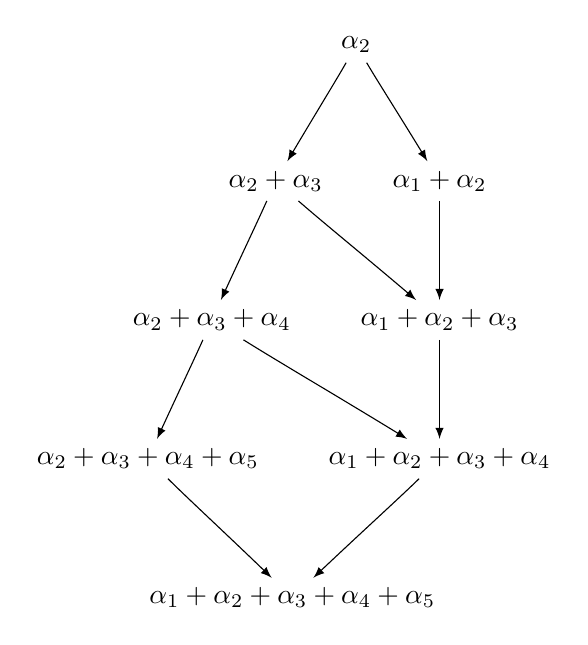
\begin{tikzpicture}[>=latex,line join=bevel,]
%%
\node (alpha2) at (118bp,206bp) [draw,draw=none] {$\alpha_{2}$};
  \node (alpha2+alpha3+alpha4+alpha5) at (43bp,57bp) [draw,draw=none] {$\alpha_{2} + \alpha_{3} + \alpha_{4} + \alpha_{5}$};
  \node (alpha2+alpha3+alpha4) at (66bp,107bp) [draw,draw=none] {$\alpha_{2} + \alpha_{3} + \alpha_{4}$};
  \node (alpha1+alpha2+alpha3+alpha4) at (148bp,57bp) [draw,draw=none] {$\alpha_{1} + \alpha_{2} + \alpha_{3} + \alpha_{4}$};
  \node (alpha1+alpha2) at (148bp,157bp) [draw,draw=none] {$\alpha_{1} + \alpha_{2}$};
  \node (alpha2+alpha3) at (89bp,157bp) [draw,draw=none] {$\alpha_{2} + \alpha_{3}$};
  \node (alpha1+alpha2+alpha3) at (148bp,107bp) [draw,draw=none] {$\alpha_{1} + \alpha_{2} + \alpha_{3}$};
  \node (alpha1+alpha2+alpha3+alpha4+alpha5) at (95bp,7bp) [draw,draw=none] {$\alpha_{1} + \alpha_{2} + \alpha_{3} + \alpha_{4} + \alpha_{5}$};
  \draw [black,->] (alpha2+alpha3+alpha4+alpha5) ..controls (57.627bp,42.498bp) and (70.704bp,30.428bp)  .. (alpha1+alpha2+alpha3+alpha4+alpha5);
  \draw [black,->] (alpha2) ..controls (125.34bp,193.5bp) and (132.69bp,181.99bp)  .. (alpha1+alpha2);
  \draw [black,->] (alpha1+alpha2+alpha3+alpha4) ..controls (133.01bp,42.426bp) and (119.5bp,30.186bp)  .. (alpha1+alpha2+alpha3+alpha4+alpha5);
  \draw [black,->] (alpha2) ..controls (110.91bp,193.5bp) and (103.8bp,181.99bp)  .. (alpha2+alpha3);
  \draw [black,->] (alpha2+alpha3) ..controls (105.77bp,142.35bp) and (121.03bp,129.94bp)  .. (alpha1+alpha2+alpha3);
  \draw [black,->] (alpha2+alpha3) ..controls (82.807bp,143.08bp) and (77.657bp,132.33bp)  .. (alpha2+alpha3+alpha4);
  \draw [black,->] (alpha2+alpha3+alpha4) ..controls (89.571bp,92.203bp) and (112.57bp,78.739bp)  .. (alpha1+alpha2+alpha3+alpha4);
  \draw [black,->] (alpha1+alpha2+alpha3) ..controls (148bp,93.293bp) and (148bp,83.024bp)  .. (alpha1+alpha2+alpha3+alpha4);
  \draw [black,->] (alpha1+alpha2) ..controls (148bp,143.29bp) and (148bp,133.02bp)  .. (alpha1+alpha2+alpha3);
  \draw [black,->] (alpha2+alpha3+alpha4) ..controls (59.807bp,93.076bp) and (54.657bp,82.328bp)  .. (alpha2+alpha3+alpha4+alpha5);
%
\end{tikzpicture} 
	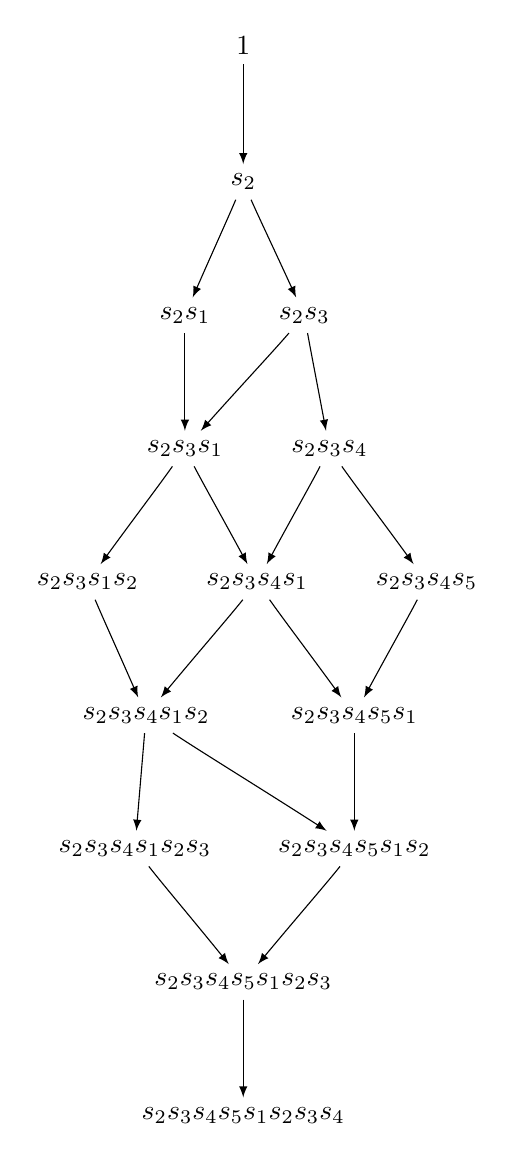
\begin{tikzpicture}[>=latex,line join=bevel,]
%%
\node (s2*s3) at (99bp,294bp) [draw,draw=none] {$s_{2}s_{3}$};
  \node (s2*s3*s4*s5*s1*s2) at (117bp,102bp) [draw,draw=none] {$s_{2}s_{3}s_{4}s_{5}s_{1}s_{2}$};
  \node (s2*s1) at (56bp,294bp) [draw,draw=none] {$s_{2}s_{1}$};
  \node (s2*s3*s4*s5*s1*s2*s3*s4) at (77bp,6bp) [draw,draw=none] {$s_{2}s_{3}s_{4}s_{5}s_{1}s_{2}s_{3}s_{4}$};
  \node (s2*s3*s1) at (56bp,246bp) [draw,draw=none] {$s_{2}s_{3}s_{1}$};
  \node (s2*s3*s4) at (108bp,246bp) [draw,draw=none] {$s_{2}s_{3}s_{4}$};
  \node (s2) at (77bp,342bp) [draw,draw=none] {$s_{2}$};
  \node (s2*s3*s4*s5*s1) at (117bp,150bp) [draw,draw=none] {$s_{2}s_{3}s_{4}s_{5}s_{1}$};
  \node (s2*s3*s4*s1) at (82bp,198bp) [draw,draw=none] {$s_{2}s_{3}s_{4}s_{1}$};
  \node (s2*s3*s1*s2) at (21bp,198bp) [draw,draw=none] {$s_{2}s_{3}s_{1}s_{2}$};
  \node (s2*s3*s4*s5*s1*s2*s3) at (77bp,54bp) [draw,draw=none] {$s_{2}s_{3}s_{4}s_{5}s_{1}s_{2}s_{3}$};
  \node (1) at (77bp,391bp) [draw,draw=none] {$1$};
  \node (s2*s3*s4*s5) at (143bp,198bp) [draw,draw=none] {$s_{2}s_{3}s_{4}s_{5}$};
  \node (s2*s3*s4*s1*s2*s3) at (38bp,102bp) [draw,draw=none] {$s_{2}s_{3}s_{4}s_{1}s_{2}s_{3}$};
  \node (s2*s3*s4*s1*s2) at (42bp,150bp) [draw,draw=none] {$s_{2}s_{3}s_{4}s_{1}s_{2}$};
  \draw [black,->] (s2*s3*s4*s5) ..controls (136.37bp,185.28bp) and (130.07bp,174.12bp)  .. (s2*s3*s4*s5*s1);
  \draw [black,->] (s2*s3*s4) ..controls (117.08bp,233.07bp) and (125.96bp,221.39bp)  .. (s2*s3*s4*s5);
  \draw [black,->] (s2*s3*s4*s1*s2) ..controls (41.005bp,137.55bp) and (40.093bp,127.07bp)  .. (s2*s3*s4*s1*s2*s3);
  \draw [black,->] (s2*s3*s4*s5*s1*s2*s3) ..controls (77bp,41.554bp) and (77bp,31.067bp)  .. (s2*s3*s4*s5*s1*s2*s3*s4);
  \draw [black,->] (s2*s3*s4*s1) ..controls (71.564bp,185bp) and (61.258bp,173.15bp)  .. (s2*s3*s4*s1*s2);
  \draw [black,->] (s2) ..controls (82.574bp,329.35bp) and (87.83bp,318.35bp)  .. (s2*s3);
  \draw [black,->] (s2*s3*s1) ..controls (62.626bp,233.28bp) and (68.935bp,222.12bp)  .. (s2*s3*s4*s1);
  \draw [black,->] (1) ..controls (77bp,377.83bp) and (77bp,367.21bp)  .. (s2);
  \draw [black,->] (s2*s3*s4*s1) ..controls (91.078bp,185.07bp) and (99.964bp,173.39bp)  .. (s2*s3*s4*s5*s1);
  \draw [black,->] (s2*s3) ..controls (87.717bp,280.93bp) and (76.473bp,268.9bp)  .. (s2*s3*s1);
  \draw [black,->] (s2*s1) ..controls (56bp,281.55bp) and (56bp,271.07bp)  .. (s2*s3*s1);
  \draw [black,->] (s2*s3*s4*s1*s2) ..controls (62.188bp,136.62bp) and (84.284bp,123.07bp)  .. (s2*s3*s4*s5*s1*s2);
  \draw [black,->] (s2) ..controls (71.68bp,329.35bp) and (66.662bp,318.35bp)  .. (s2*s1);
  \draw [black,->] (s2*s3*s4*s1*s2*s3) ..controls (48.175bp,88.999bp) and (58.224bp,77.147bp)  .. (s2*s3*s4*s5*s1*s2*s3);
  \draw [black,->] (s2*s3*s4*s5*s1*s2) ..controls (106.56bp,88.999bp) and (96.258bp,77.147bp)  .. (s2*s3*s4*s5*s1*s2*s3);
  \draw [black,->] (s2*s3*s4) ..controls (101.37bp,233.28bp) and (95.065bp,222.12bp)  .. (s2*s3*s4*s1);
  \draw [black,->] (s2*s3*s1*s2) ..controls (26.32bp,185.35bp) and (31.338bp,174.35bp)  .. (s2*s3*s4*s1*s2);
  \draw [black,->] (s2*s3*s4*s5*s1) ..controls (117bp,137.55bp) and (117bp,127.07bp)  .. (s2*s3*s4*s5*s1*s2);
  \draw [black,->] (s2*s3) ..controls (101.24bp,281.55bp) and (103.29bp,271.07bp)  .. (s2*s3*s4);
  \draw [black,->] (s2*s3*s1) ..controls (46.922bp,233.07bp) and (38.036bp,221.39bp)  .. (s2*s3*s1*s2);
%
\end{tikzpicture} 
  \caption{Poset of noncompact roots and the Bruhat graph for $\mathrm{SU}(2,4)$}
\end{figure} 

\begin{figure}[H]
  \centering 
	\resizebox{\textwidth}{!}{
  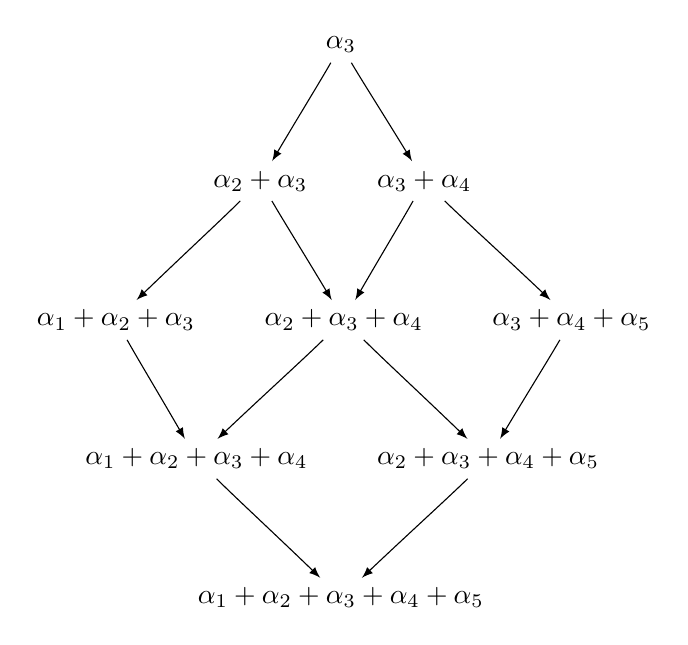
\begin{tikzpicture}[>=latex,line join=bevel,]
%%
\node (alpha3) at (113bp,206bp) [draw,draw=none] {$\alpha_{3}$};
  \node (alpha2+alpha3+alpha4+alpha5) at (166bp,57bp) [draw,draw=none] {$\alpha_{2} + \alpha_{3} + \alpha_{4} + \alpha_{5}$};
  \node (alpha2+alpha3+alpha4) at (114bp,107bp) [draw,draw=none] {$\alpha_{2} + \alpha_{3} + \alpha_{4}$};
  \node (alpha1+alpha2+alpha3+alpha4) at (61bp,57bp) [draw,draw=none] {$\alpha_{1} + \alpha_{2} + \alpha_{3} + \alpha_{4}$};
  \node (alpha2+alpha3) at (84bp,157bp) [draw,draw=none] {$\alpha_{2} + \alpha_{3}$};
  \node (alpha1+alpha2+alpha3) at (32bp,107bp) [draw,draw=none] {$\alpha_{1} + \alpha_{2} + \alpha_{3}$};
  \node (alpha1+alpha2+alpha3+alpha4+alpha5) at (113bp,7bp) [draw,draw=none] {$\alpha_{1} + \alpha_{2} + \alpha_{3} + \alpha_{4} + \alpha_{5}$};
  \node (alpha3+alpha4) at (143bp,157bp) [draw,draw=none] {$\alpha_{3} + \alpha_{4}$};
  \node (alpha3+alpha4+alpha5) at (196bp,107bp) [draw,draw=none] {$\alpha_{3} + \alpha_{4} + \alpha_{5}$};
  \draw [black,->] (alpha2+alpha3+alpha4+alpha5) ..controls (151.01bp,42.426bp) and (137.5bp,30.186bp)  .. (alpha1+alpha2+alpha3+alpha4+alpha5);
  \draw [black,->] (alpha3) ..controls (120.34bp,193.5bp) and (127.69bp,181.99bp)  .. (alpha3+alpha4);
  \draw [black,->] (alpha3+alpha4) ..controls (157.99bp,142.43bp) and (171.5bp,130.19bp)  .. (alpha3+alpha4+alpha5);
  \draw [black,->] (alpha1+alpha2+alpha3) ..controls (39.895bp,92.932bp) and (46.585bp,81.859bp)  .. (alpha1+alpha2+alpha3+alpha4);
  \draw [black,->] (alpha2+alpha3) ..controls (69.373bp,142.5bp) and (56.296bp,130.43bp)  .. (alpha1+alpha2+alpha3);
  \draw [black,->] (alpha2+alpha3) ..controls (92.168bp,142.93bp) and (99.088bp,131.86bp)  .. (alpha2+alpha3+alpha4);
  \draw [black,->] (alpha2+alpha3+alpha4) ..controls (99.012bp,92.426bp) and (85.497bp,80.186bp)  .. (alpha1+alpha2+alpha3+alpha4);
  \draw [black,->] (alpha3+alpha4+alpha5) ..controls (187.83bp,92.932bp) and (180.91bp,81.859bp)  .. (alpha2+alpha3+alpha4+alpha5);
  \draw [black,->] (alpha3) ..controls (105.91bp,193.5bp) and (98.803bp,181.99bp)  .. (alpha2+alpha3);
  \draw [black,->] (alpha3+alpha4) ..controls (135.1bp,142.93bp) and (128.41bp,131.86bp)  .. (alpha2+alpha3+alpha4);
  \draw [black,->] (alpha2+alpha3+alpha4) ..controls (128.63bp,92.498bp) and (141.7bp,80.428bp)  .. (alpha2+alpha3+alpha4+alpha5);
  \draw [black,->] (alpha1+alpha2+alpha3+alpha4) ..controls (75.627bp,42.498bp) and (88.704bp,30.428bp)  .. (alpha1+alpha2+alpha3+alpha4+alpha5);
%
\end{tikzpicture} 
	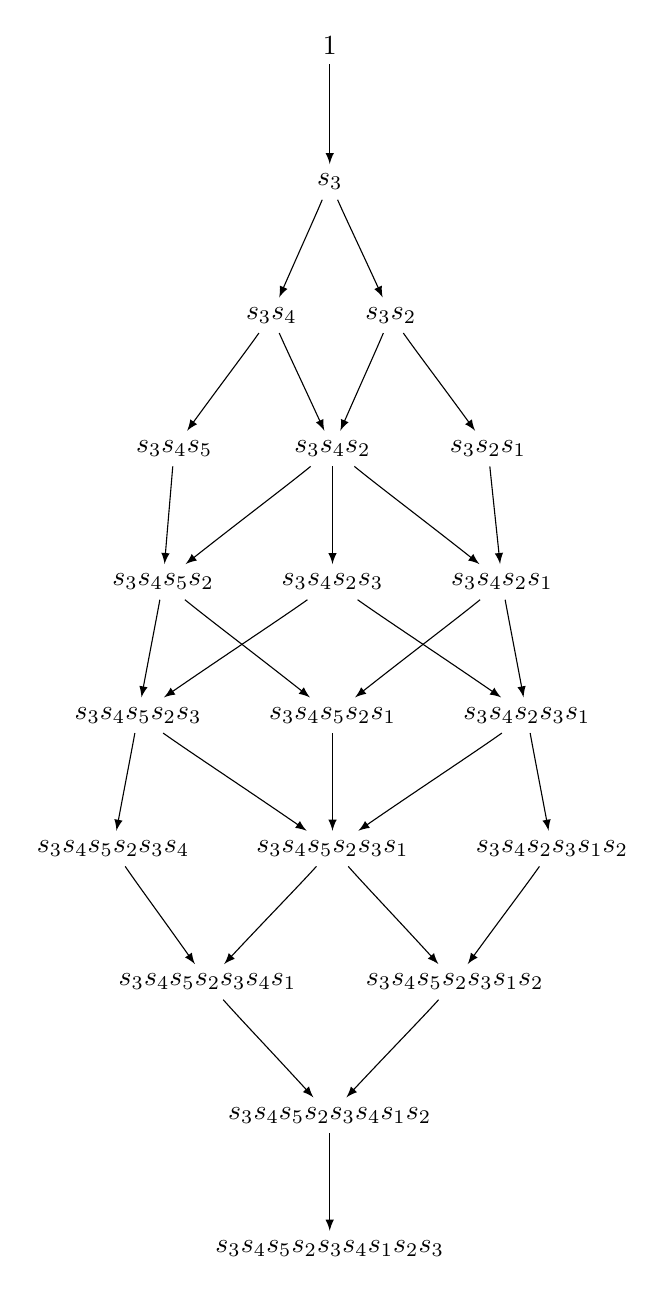
\begin{tikzpicture}[>=latex,line join=bevel,]
%%
\node (s3*s4*s5*s2*s3*s4) at (30bp,150bp) [draw,draw=none] {$s_{3}s_{4}s_{5}s_{2}s_{3}s_{4}$};
  \node (s3*s4*s5*s2*s3*s4*s1*s2) at (108bp,54bp) [draw,draw=none] {$s_{3}s_{4}s_{5}s_{2}s_{3}s_{4}s_{1}s_{2}$};
  \node (s3*s4*s5*s2*s3*s1) at (109bp,150bp) [draw,draw=none] {$s_{3}s_{4}s_{5}s_{2}s_{3}s_{1}$};
  \node (s3*s4*s5) at (52bp,294bp) [draw,draw=none] {$s_{3}s_{4}s_{5}$};
  \node (s3) at (108bp,390bp) [draw,draw=none] {$s_{3}$};
  \node (s3*s4*s5*s2*s3*s4*s1*s2*s3) at (108bp,6bp) [draw,draw=none] {$s_{3}s_{4}s_{5}s_{2}s_{3}s_{4}s_{1}s_{2}s_{3}$};
  \node (s3*s4*s2) at (109bp,294bp) [draw,draw=none] {$s_{3}s_{4}s_{2}$};
  \node (s3*s4*s5*s2*s3) at (39bp,198bp) [draw,draw=none] {$s_{3}s_{4}s_{5}s_{2}s_{3}$};
  \node (s3*s4*s5*s2) at (48bp,246bp) [draw,draw=none] {$s_{3}s_{4}s_{5}s_{2}$};
  \node (s3*s4*s5*s2*s1) at (109bp,198bp) [draw,draw=none] {$s_{3}s_{4}s_{5}s_{2}s_{1}$};
  \node (s3*s4*s5*s2*s3*s4*s1) at (64bp,102bp) [draw,draw=none] {$s_{3}s_{4}s_{5}s_{2}s_{3}s_{4}s_{1}$};
  \node (1) at (108bp,439bp) [draw,draw=none] {$1$};
  \node (s3*s4*s2*s3*s1*s2) at (188bp,150bp) [draw,draw=none] {$s_{3}s_{4}s_{2}s_{3}s_{1}s_{2}$};
  \node (s3*s4*s5*s2*s3*s1*s2) at (153bp,102bp) [draw,draw=none] {$s_{3}s_{4}s_{5}s_{2}s_{3}s_{1}s_{2}$};
  \node (s3*s2) at (130bp,342bp) [draw,draw=none] {$s_{3}s_{2}$};
  \node (s3*s2*s1) at (165bp,294bp) [draw,draw=none] {$s_{3}s_{2}s_{1}$};
  \node (s3*s4) at (87bp,342bp) [draw,draw=none] {$s_{3}s_{4}$};
  \node (s3*s4*s2*s3) at (109bp,246bp) [draw,draw=none] {$s_{3}s_{4}s_{2}s_{3}$};
  \node (s3*s4*s2*s3*s1) at (179bp,198bp) [draw,draw=none] {$s_{3}s_{4}s_{2}s_{3}s_{1}$};
  \node (s3*s4*s2*s1) at (170bp,246bp) [draw,draw=none] {$s_{3}s_{4}s_{2}s_{1}$};
  \draw [black,->] (s3*s2) ..controls (139.08bp,329.07bp) and (147.96bp,317.39bp)  .. (s3*s2*s1);
  \draw [black,->] (s3*s4*s5*s2) ..controls (64.466bp,232.58bp) and (81.602bp,219.66bp)  .. (s3*s4*s5*s2*s1);
  \draw [black,->] (s3*s4) ..controls (92.574bp,329.35bp) and (97.83bp,318.35bp)  .. (s3*s4*s2);
  \draw [black,->] (s3*s4*s5*s2*s3*s1) ..controls (97.124bp,136.86bp) and (85.185bp,124.66bp)  .. (s3*s4*s5*s2*s3*s4*s1);
  \draw [black,->] (s3*s4*s5*s2*s3) ..controls (57.738bp,184.69bp) and (78.077bp,171.32bp)  .. (s3*s4*s5*s2*s3*s1);
  \draw [black,->] (s3*s4*s2*s1) ..controls (172.24bp,233.55bp) and (174.29bp,223.07bp)  .. (s3*s4*s2*s3*s1);
  \draw [black,->] (s3*s4*s2*s3*s1) ..controls (181.24bp,185.55bp) and (183.29bp,175.07bp)  .. (s3*s4*s2*s3*s1*s2);
  \draw [black,->] (s3*s4*s5*s2*s3*s1*s2) ..controls (141.12bp,88.86bp) and (129.18bp,76.656bp)  .. (s3*s4*s5*s2*s3*s4*s1*s2);
  \draw [black,->] (s3*s4*s5*s2*s1) ..controls (109bp,185.55bp) and (109bp,175.07bp)  .. (s3*s4*s5*s2*s3*s1);
  \draw [black,->] (s3*s4*s2) ..controls (92.534bp,280.58bp) and (75.398bp,267.66bp)  .. (s3*s4*s5*s2);
  \draw [black,->] (1) ..controls (108bp,425.83bp) and (108bp,415.21bp)  .. (s3);
  \draw [black,->] (s3*s4*s2*s3*s1*s2) ..controls (178.92bp,137.07bp) and (170.04bp,125.39bp)  .. (s3*s4*s5*s2*s3*s1*s2);
  \draw [black,->] (s3*s2) ..controls (124.68bp,329.35bp) and (119.66bp,318.35bp)  .. (s3*s4*s2);
  \draw [black,->] (s3*s4*s5*s2*s3*s4*s1*s2) ..controls (108bp,41.554bp) and (108bp,31.067bp)  .. (s3*s4*s5*s2*s3*s4*s1*s2*s3);
  \draw [black,->] (s3) ..controls (113.57bp,377.35bp) and (118.83bp,366.35bp)  .. (s3*s2);
  \draw [black,->] (s3*s4*s2) ..controls (125.47bp,280.58bp) and (142.6bp,267.66bp)  .. (s3*s4*s2*s1);
  \draw [black,->] (s3*s4*s5*s2) ..controls (45.76bp,233.55bp) and (43.709bp,223.07bp)  .. (s3*s4*s5*s2*s3);
  \draw [black,->] (s3*s4*s2*s3) ..controls (127.74bp,232.69bp) and (148.08bp,219.32bp)  .. (s3*s4*s2*s3*s1);
  \draw [black,->] (s3*s4*s5*s2*s3*s4*s1) ..controls (75.546bp,88.93bp) and (87.051bp,76.902bp)  .. (s3*s4*s5*s2*s3*s4*s1*s2);
  \draw [black,->] (s3*s4*s5) ..controls (51.005bp,281.55bp) and (50.093bp,271.07bp)  .. (s3*s4*s5*s2);
  \draw [black,->] (s3*s4*s5*s2*s3) ..controls (36.76bp,185.55bp) and (34.709bp,175.07bp)  .. (s3*s4*s5*s2*s3*s4);
  \draw [black,->] (s3*s4*s5*s2*s3*s4) ..controls (38.768bp,137.14bp) and (47.271bp,125.63bp)  .. (s3*s4*s5*s2*s3*s4*s1);
  \draw [black,->] (s3*s4*s2*s3) ..controls (90.262bp,232.69bp) and (69.923bp,219.32bp)  .. (s3*s4*s5*s2*s3);
  \draw [black,->] (s3*s4*s5*s2*s3*s1) ..controls (120.55bp,136.93bp) and (132.05bp,124.9bp)  .. (s3*s4*s5*s2*s3*s1*s2);
  \draw [black,->] (s3*s4*s2*s3*s1) ..controls (160.26bp,184.69bp) and (139.92bp,171.32bp)  .. (s3*s4*s5*s2*s3*s1);
  \draw [black,->] (s3) ..controls (102.68bp,377.35bp) and (97.662bp,366.35bp)  .. (s3*s4);
  \draw [black,->] (s3*s4) ..controls (77.922bp,329.07bp) and (69.036bp,317.39bp)  .. (s3*s4*s5);
  \draw [black,->] (s3*s2*s1) ..controls (166.24bp,281.55bp) and (167.38bp,271.07bp)  .. (s3*s4*s2*s1);
  \draw [black,->] (s3*s4*s2) ..controls (109bp,281.55bp) and (109bp,271.07bp)  .. (s3*s4*s2*s3);
  \draw [black,->] (s3*s4*s2*s1) ..controls (153.53bp,232.58bp) and (136.4bp,219.66bp)  .. (s3*s4*s5*s2*s1);
%
\end{tikzpicture} 
	}
  \caption{Poset of noncompact roots and the Bruhat graphfor $\mathrm{SU}(3,3)$}
\end{figure} 

\begin{figure}[H]
  \centering 
  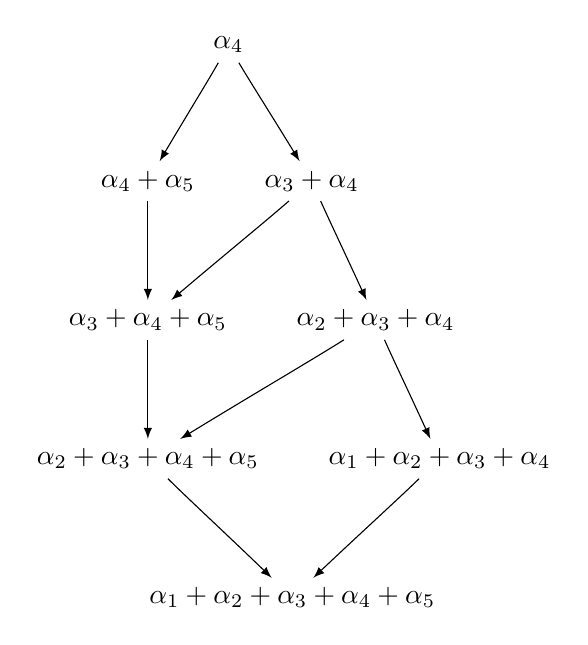
\begin{tikzpicture}[>=latex,line join=bevel,]
%%
\node (alpha2+alpha3+alpha4+alpha5) at (43bp,57bp) [draw,draw=none] {$\alpha_{2} + \alpha_{3} + \alpha_{4} + \alpha_{5}$};
  \node (alpha2+alpha3+alpha4) at (125bp,107bp) [draw,draw=none] {$\alpha_{2} + \alpha_{3} + \alpha_{4}$};
  \node (alpha4) at (72bp,206bp) [draw,draw=none] {$\alpha_{4}$};
  \node (alpha1+alpha2+alpha3+alpha4) at (148bp,57bp) [draw,draw=none] {$\alpha_{1} + \alpha_{2} + \alpha_{3} + \alpha_{4}$};
  \node (alpha4+alpha5) at (43bp,157bp) [draw,draw=none] {$\alpha_{4} + \alpha_{5}$};
  \node (alpha1+alpha2+alpha3+alpha4+alpha5) at (95bp,7bp) [draw,draw=none] {$\alpha_{1} + \alpha_{2} + \alpha_{3} + \alpha_{4} + \alpha_{5}$};
  \node (alpha3+alpha4) at (102bp,157bp) [draw,draw=none] {$\alpha_{3} + \alpha_{4}$};
  \node (alpha3+alpha4+alpha5) at (43bp,107bp) [draw,draw=none] {$\alpha_{3} + \alpha_{4} + \alpha_{5}$};
  \draw [black,->] (alpha2+alpha3+alpha4) ..controls (131.19bp,93.076bp) and (136.34bp,82.328bp)  .. (alpha1+alpha2+alpha3+alpha4);
  \draw [black,->] (alpha2+alpha3+alpha4+alpha5) ..controls (57.627bp,42.498bp) and (70.704bp,30.428bp)  .. (alpha1+alpha2+alpha3+alpha4+alpha5);
  \draw [black,->] (alpha1+alpha2+alpha3+alpha4) ..controls (133.01bp,42.426bp) and (119.5bp,30.186bp)  .. (alpha1+alpha2+alpha3+alpha4+alpha5);
  \draw [black,->] (alpha4) ..controls (64.906bp,193.5bp) and (57.803bp,181.99bp)  .. (alpha4+alpha5);
  \draw [black,->] (alpha4+alpha5) ..controls (43bp,143.29bp) and (43bp,133.02bp)  .. (alpha3+alpha4+alpha5);
  \draw [black,->] (alpha3+alpha4+alpha5) ..controls (43bp,93.293bp) and (43bp,83.024bp)  .. (alpha2+alpha3+alpha4+alpha5);
  \draw [black,->] (alpha3+alpha4) ..controls (108.19bp,143.08bp) and (113.34bp,132.33bp)  .. (alpha2+alpha3+alpha4);
  \draw [black,->] (alpha4) ..controls (79.339bp,193.5bp) and (86.686bp,181.99bp)  .. (alpha3+alpha4);
  \draw [black,->] (alpha3+alpha4) ..controls (85.226bp,142.35bp) and (69.971bp,129.94bp)  .. (alpha3+alpha4+alpha5);
  \draw [black,->] (alpha2+alpha3+alpha4) ..controls (101.43bp,92.203bp) and (78.43bp,78.739bp)  .. (alpha2+alpha3+alpha4+alpha5);
%
\end{tikzpicture} 
	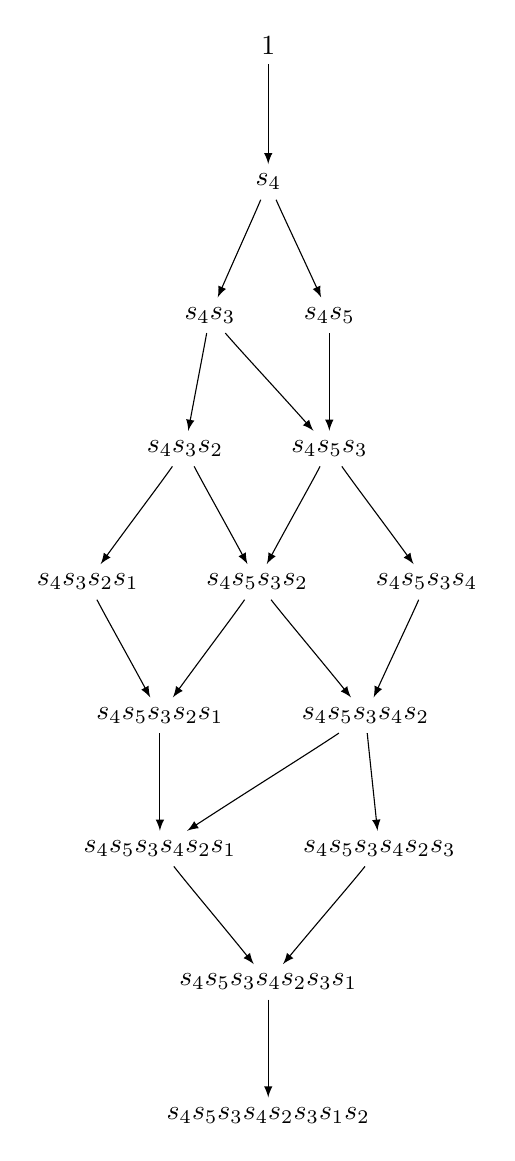
\begin{tikzpicture}[>=latex,line join=bevel,]
%%
\node (s4*s5*s3*s4*s2*s3) at (126bp,102bp) [draw,draw=none] {$s_{4}s_{5}s_{3}s_{4}s_{2}s_{3}$};
  \node (s4*s5*s3*s4) at (143bp,198bp) [draw,draw=none] {$s_{4}s_{5}s_{3}s_{4}$};
  \node (s4*s5*s3*s4*s2*s1) at (47bp,102bp) [draw,draw=none] {$s_{4}s_{5}s_{3}s_{4}s_{2}s_{1}$};
  \node (s4*s5*s3*s2) at (82bp,198bp) [draw,draw=none] {$s_{4}s_{5}s_{3}s_{2}$};
  \node (s4*s3*s2) at (56bp,246bp) [draw,draw=none] {$s_{4}s_{3}s_{2}$};
  \node (s4*s3) at (65bp,294bp) [draw,draw=none] {$s_{4}s_{3}$};
  \node (s4*s5) at (108bp,294bp) [draw,draw=none] {$s_{4}s_{5}$};
  \node (s4*s5*s3*s4*s2*s3*s1) at (86bp,54bp) [draw,draw=none] {$s_{4}s_{5}s_{3}s_{4}s_{2}s_{3}s_{1}$};
  \node (s4) at (86bp,342bp) [draw,draw=none] {$s_{4}$};
  \node (1) at (86bp,391bp) [draw,draw=none] {$1$};
  \node (s4*s5*s3*s4*s2) at (121bp,150bp) [draw,draw=none] {$s_{4}s_{5}s_{3}s_{4}s_{2}$};
  \node (s4*s5*s3*s2*s1) at (47bp,150bp) [draw,draw=none] {$s_{4}s_{5}s_{3}s_{2}s_{1}$};
  \node (s4*s5*s3*s4*s2*s3*s1*s2) at (86bp,6bp) [draw,draw=none] {$s_{4}s_{5}s_{3}s_{4}s_{2}s_{3}s_{1}s_{2}$};
  \node (s4*s5*s3) at (108bp,246bp) [draw,draw=none] {$s_{4}s_{5}s_{3}$};
  \node (s4*s3*s2*s1) at (21bp,198bp) [draw,draw=none] {$s_{4}s_{3}s_{2}s_{1}$};
  \draw [black,->] (s4*s5*s3*s2) ..controls (72.922bp,185.07bp) and (64.036bp,173.39bp)  .. (s4*s5*s3*s2*s1);
  \draw [black,->] (s4*s3) ..controls (62.76bp,281.55bp) and (60.709bp,271.07bp)  .. (s4*s3*s2);
  \draw [black,->] (s4*s5*s3) ..controls (117.08bp,233.07bp) and (125.96bp,221.39bp)  .. (s4*s5*s3*s4);
  \draw [black,->] (s4*s3*s2) ..controls (62.626bp,233.28bp) and (68.935bp,222.12bp)  .. (s4*s5*s3*s2);
  \draw [black,->] (s4*s5) ..controls (108bp,281.55bp) and (108bp,271.07bp)  .. (s4*s5*s3);
  \draw [black,->] (s4*s5*s3*s2*s1) ..controls (47bp,137.55bp) and (47bp,127.07bp)  .. (s4*s5*s3*s4*s2*s1);
  \draw [black,->] (s4*s3*s2*s1) ..controls (27.626bp,185.28bp) and (33.935bp,174.12bp)  .. (s4*s5*s3*s2*s1);
  \draw [black,->] (s4) ..controls (91.574bp,329.35bp) and (96.83bp,318.35bp)  .. (s4*s5);
  \draw [black,->] (s4*s5*s3*s4*s2*s3) ..controls (115.56bp,88.999bp) and (105.26bp,77.147bp)  .. (s4*s5*s3*s4*s2*s3*s1);
  \draw [black,->] (s4*s5*s3*s4*s2*s1) ..controls (57.175bp,88.999bp) and (67.224bp,77.147bp)  .. (s4*s5*s3*s4*s2*s3*s1);
  \draw [black,->] (s4) ..controls (80.68bp,329.35bp) and (75.662bp,318.35bp)  .. (s4*s3);
  \draw [black,->] (s4*s5*s3*s4) ..controls (137.43bp,185.35bp) and (132.17bp,174.35bp)  .. (s4*s5*s3*s4*s2);
  \draw [black,->] (s4*s5*s3*s4*s2) ..controls (101.08bp,136.62bp) and (79.28bp,123.07bp)  .. (s4*s5*s3*s4*s2*s1);
  \draw [black,->] (s4*s5*s3) ..controls (101.37bp,233.28bp) and (95.065bp,222.12bp)  .. (s4*s5*s3*s2);
  \draw [black,->] (s4*s5*s3*s4*s2) ..controls (122.24bp,137.55bp) and (123.38bp,127.07bp)  .. (s4*s5*s3*s4*s2*s3);
  \draw [black,->] (s4*s3) ..controls (76.283bp,280.93bp) and (87.527bp,268.9bp)  .. (s4*s5*s3);
  \draw [black,->] (1) ..controls (86bp,377.83bp) and (86bp,367.21bp)  .. (s4);
  \draw [black,->] (s4*s5*s3*s2) ..controls (92.175bp,185bp) and (102.22bp,173.15bp)  .. (s4*s5*s3*s4*s2);
  \draw [black,->] (s4*s3*s2) ..controls (46.922bp,233.07bp) and (38.036bp,221.39bp)  .. (s4*s3*s2*s1);
  \draw [black,->] (s4*s5*s3*s4*s2*s3*s1) ..controls (86bp,41.554bp) and (86bp,31.067bp)  .. (s4*s5*s3*s4*s2*s3*s1*s2);
%
\end{tikzpicture} 
  \caption{Poset of noncompact roots and the Bruhat graph for $\mathrm{SU}(4,2)$}
\end{figure} 

\begin{figure}[H]
  \centering 
  \begin{tikzpicture}[>=latex,line join=bevel,]
%%
\node (alpha1+alpha2+alpha3+alpha4+alpha5) at (55bp,7bp) [draw,draw=none] {$\alpha_{1} + \alpha_{2} + \alpha_{3} + \alpha_{4} + \alpha_{5}$};
  \node (alpha2+alpha3+alpha4+alpha5) at (55bp,57bp) [draw,draw=none] {$\alpha_{2} + \alpha_{3} + \alpha_{4} + \alpha_{5}$};
  \node (alpha5) at (55bp,206bp) [draw,draw=none] {$\alpha_{5}$};
  \node (alpha3+alpha4+alpha5) at (55bp,107bp) [draw,draw=none] {$\alpha_{3} + \alpha_{4} + \alpha_{5}$};
  \node (alpha4+alpha5) at (55bp,157bp) [draw,draw=none] {$\alpha_{4} + \alpha_{5}$};
  \draw [black,->] (alpha4+alpha5) ..controls (55bp,143.29bp) and (55bp,133.02bp)  .. (alpha3+alpha4+alpha5);
  \draw [black,->] (alpha3+alpha4+alpha5) ..controls (55bp,93.293bp) and (55bp,83.024bp)  .. (alpha2+alpha3+alpha4+alpha5);
  \draw [black,->] (alpha5) ..controls (55bp,193.84bp) and (55bp,183.19bp)  .. (alpha4+alpha5);
  \draw [black,->] (alpha2+alpha3+alpha4+alpha5) ..controls (55bp,43.293bp) and (55bp,33.024bp)  .. (alpha1+alpha2+alpha3+alpha4+alpha5);
%
\end{tikzpicture}
	\begin{tikzpicture}[>=latex,line join=bevel,]
%%
\node (s5*s4*s3*s2*s1) at (26bp,6bp) [draw,draw=none] {$s_{5}s_{4}s_{3}s_{2}s_{1}$};
  \node (s5) at (26bp,198bp) [draw,draw=none] {$s_{5}$};
  \node (1) at (26bp,247bp) [draw,draw=none] {$1$};
  \node (s5*s4*s3*s2) at (26bp,54bp) [draw,draw=none] {$s_{5}s_{4}s_{3}s_{2}$};
  \node (s5*s4*s3) at (26bp,102bp) [draw,draw=none] {$s_{5}s_{4}s_{3}$};
  \node (s5*s4) at (26bp,150bp) [draw,draw=none] {$s_{5}s_{4}$};
  \draw [black,->] (s5*s4*s3*s2) ..controls (26bp,41.554bp) and (26bp,31.067bp)  .. (s5*s4*s3*s2*s1);
  \draw [black,->] (1) ..controls (26bp,233.83bp) and (26bp,223.21bp)  .. (s5);
  \draw [black,->] (s5) ..controls (26bp,185.55bp) and (26bp,175.07bp)  .. (s5*s4);
  \draw [black,->] (s5*s4*s3) ..controls (26bp,89.554bp) and (26bp,79.067bp)  .. (s5*s4*s3*s2);
  \draw [black,->] (s5*s4) ..controls (26bp,137.55bp) and (26bp,127.07bp)  .. (s5*s4*s3);
%
\end{tikzpicture}
  \caption{Poset of noncompact roots and the Bruhat graph for $\mathrm{SU}(5,1)$}
\end{figure} 

\begin{figure}[H]
  \centering 
  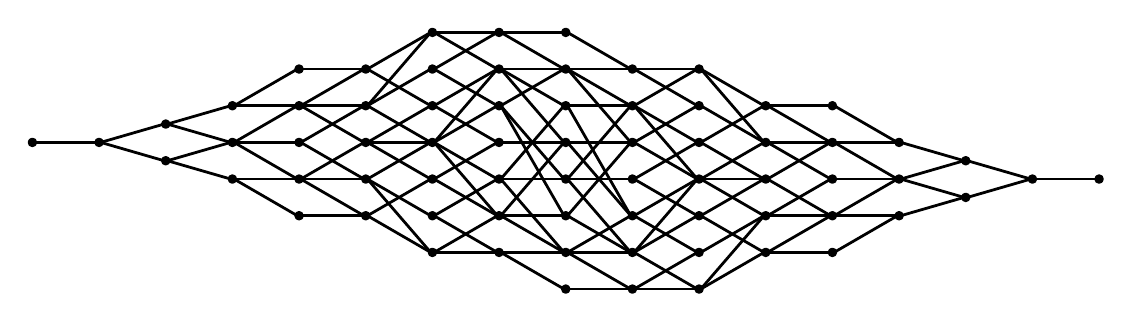
\begin{tikzpicture}[=latex,line join=bevel,scale=0.6]
  \pgfsetlinewidth{1bp}
%%
\pgfsetcolor{black}
  % Edge: s_4*s_5*s_6*s_7*s_3*s_4*s_5*s_2 - s_4*s_5*s_6*s_7*s_3*s_4*s_5*s_2*s_3
  \draw [-] (323.94bp,132.46bp) .. controls (327.67bp,130.3bp) and (341.69bp,122.18bp)  .. (360.22bp,111.45bp);
  % Edge: s_4*s_5*s_6*s_3*s_4*s_2*s_3 - s_4*s_5*s_6*s_3*s_4*s_5*s_2*s_3
  \draw [-] (283.94bp,67bp) .. controls (287.42bp,67bp) and (299.87bp,67bp)  .. (319.65bp,67bp);
  % Edge: s_4*s_5*s_3 - s_4*s_5*s_3*s_2
  \draw [-] (123.94bp,88.456bp) .. controls (127.67bp,86.297bp) and (141.69bp,78.178bp)  .. (160.22bp,67.449bp);
  % Edge: s_4*s_5*s_6*s_3*s_4*s_5*s_2*s_3*s_4 - s_4*s_5*s_6*s_7*s_3*s_4*s_5*s_2*s_3*s_4
  \draw [-] (363.94bp,67.544bp) .. controls (367.67bp,69.703bp) and (381.69bp,77.822bp)  .. (400.22bp,88.551bp);
  % Edge: s_4*s_5*s_6*s_7*s_3*s_4*s_5*s_6*s_2*s_3*s_4*s_1 - s_4*s_5*s_6*s_7*s_3*s_4*s_5*s_6*s_2*s_3*s_4*s_1*s_2
  \draw [-] (483.94bp,88.456bp) .. controls (487.67bp,86.297bp) and (501.69bp,78.178bp)  .. (520.22bp,67.449bp);
  % Edge: s_4 - s_4*s_3
  \draw [-] (43.939bp,88.728bp) .. controls (47.499bp,87.698bp) and (60.446bp,83.95bp)  .. (79.648bp,78.391bp);
  % Edge: s_4*s_5*s_6*s_7*s_3*s_2*s_1 - s_4*s_5*s_6*s_7*s_3*s_4*s_2*s_1
  \draw [-] (283.94bp,89bp) .. controls (287.42bp,89bp) and (299.87bp,89bp)  .. (319.65bp,89bp);
  % Edge: s_4*s_5*s_6*s_7*s_3*s_4*s_5*s_6*s_2*s_3*s_4*s_1*s_2 - s_4*s_5*s_6*s_7*s_3*s_4*s_5*s_6*s_2*s_3*s_4*s_1*s_2*s_3
  \draw [-] (523.94bp,66.728bp) .. controls (527.5bp,65.698bp) and (540.45bp,61.95bp)  .. (559.65bp,56.391bp);
  % Edge: s_4*s_5*s_6*s_3*s_4*s_5*s_2*s_1 - s_4*s_5*s_6*s_7*s_3*s_4*s_5*s_2*s_1
  \draw [-] (323.66bp,45.764bp) .. controls (327.16bp,49.818bp) and (343.78bp,69.061bp)  .. (360.2bp,88.071bp);
  % Edge: s_4*s_5*s_6*s_7*s_3*s_4*s_5*s_6*s_2*s_3*s_4*s_1*s_2 - s_4*s_5*s_6*s_7*s_3*s_4*s_5*s_6*s_2*s_3*s_4*s_5*s_1*s_2
  \draw [-] (523.94bp,67.272bp) .. controls (527.5bp,68.302bp) and (540.45bp,72.05bp)  .. (559.65bp,77.609bp);
  % Edge: s_4*s_5*s_3*s_2*s_1 - s_4*s_5*s_3*s_4*s_2*s_1
  \draw [-] (203.94bp,44.456bp) .. controls (207.67bp,42.297bp) and (221.69bp,34.178bp)  .. (240.22bp,23.449bp);
  % Edge: s_4*s_5*s_6*s_7*s_3*s_4*s_2*s_3 - s_4*s_5*s_6*s_7*s_3*s_4*s_5*s_2*s_3
  \draw [-] (323.94bp,111bp) .. controls (327.42bp,111bp) and (339.87bp,111bp)  .. (359.65bp,111bp);
  % Edge: s_4*s_5*s_6*s_7*s_3*s_4*s_5*s_2*s_3*s_4*s_1*s_2 - s_4*s_5*s_6*s_7*s_3*s_4*s_5*s_2*s_3*s_4*s_1*s_2*s_3
  \draw [-] (483.94bp,45bp) .. controls (487.42bp,45bp) and (499.87bp,45bp)  .. (519.65bp,45bp);
  % Edge: s_4*s_5*s_6*s_3*s_4*s_5 - s_4*s_5*s_6*s_3*s_4*s_5*s_2
  \draw [-] (243.94bp,132.46bp) .. controls (247.67bp,130.3bp) and (261.69bp,122.18bp)  .. (280.22bp,111.45bp);
  % Edge: s_4*s_5*s_6*s_7*s_3*s_4*s_5*s_6*s_2*s_3*s_1 - s_4*s_5*s_6*s_7*s_3*s_4*s_5*s_6*s_2*s_3*s_1*s_2
  \draw [-] (443.94bp,88.456bp) .. controls (447.67bp,86.297bp) and (461.69bp,78.178bp)  .. (480.22bp,67.449bp);
  % Edge: s_4*s_5*s_3*s_2*s_1 - s_4*s_5*s_6*s_3*s_2*s_1
  \draw [-] (203.94bp,45.544bp) .. controls (207.67bp,47.703bp) and (221.69bp,55.822bp)  .. (240.22bp,66.551bp);
  % Edge: s_4*s_5*s_6*s_3*s_2 - s_4*s_5*s_6*s_3*s_2*s_1
  \draw [-] (203.94bp,88.456bp) .. controls (207.67bp,86.297bp) and (221.69bp,78.178bp)  .. (240.22bp,67.449bp);
  % Edge: s_4*s_5*s_6*s_7*s_3 - s_4*s_5*s_6*s_7*s_3*s_2
  \draw [-] (203.94bp,132.46bp) .. controls (207.67bp,130.3bp) and (221.69bp,122.18bp)  .. (240.22bp,111.45bp);
  % Edge: s_4*s_5*s_6*s_3 - s_4*s_5*s_6*s_7*s_3
  \draw [-] (163.94bp,111.54bp) .. controls (167.67bp,113.7bp) and (181.69bp,121.82bp)  .. (200.22bp,132.55bp);
  % Edge: s_4*s_5*s_6*s_3*s_4 - s_4*s_5*s_6*s_7*s_3*s_4
  \draw [-] (203.66bp,111.76bp) .. controls (207.16bp,115.82bp) and (223.78bp,135.06bp)  .. (240.2bp,154.07bp);
  % Edge: s_4*s_5*s_6*s_7*s_3*s_4*s_5*s_6*s_2*s_3*s_4*s_5*s_1 - s_4*s_5*s_6*s_7*s_3*s_4*s_5*s_6*s_2*s_3*s_4*s_5*s_1*s_2
  \draw [-] (523.94bp,88.728bp) .. controls (527.5bp,87.698bp) and (540.45bp,83.95bp)  .. (559.65bp,78.391bp);
  % Edge: s_4*s_5*s_6*s_7*s_3*s_4*s_2*s_3*s_1 - s_4*s_5*s_6*s_7*s_3*s_4*s_5*s_2*s_3*s_1
  \draw [-] (363.94bp,45.544bp) .. controls (367.67bp,47.703bp) and (381.69bp,55.822bp)  .. (400.22bp,66.551bp);
  % Edge: s_4*s_5*s_6*s_3*s_2*s_1 - s_4*s_5*s_6*s_7*s_3*s_2*s_1
  \draw [-] (243.94bp,67.544bp) .. controls (247.67bp,69.703bp) and (261.69bp,77.822bp)  .. (280.22bp,88.551bp);
  % Edge: s_4*s_5*s_6*s_7*s_3*s_4*s_5*s_2*s_1 - s_4*s_5*s_6*s_7*s_3*s_4*s_5*s_6*s_2*s_1
  \draw [-] (363.94bp,89.544bp) .. controls (367.67bp,91.703bp) and (381.69bp,99.822bp)  .. (400.22bp,110.55bp);
  % Edge: s_4*s_5*s_6*s_7*s_3*s_4*s_5*s_2*s_3*s_1 - s_4*s_5*s_6*s_7*s_3*s_4*s_5*s_2*s_3*s_4*s_1
  \draw [-] (403.94bp,67bp) .. controls (407.42bp,67bp) and (419.87bp,67bp)  .. (439.65bp,67bp);
  % Edge: s_4*s_5*s_6*s_3*s_4*s_2 - s_4*s_5*s_6*s_7*s_3*s_4*s_2
  \draw [-] (243.66bp,89.764bp) .. controls (247.16bp,93.818bp) and (263.78bp,113.06bp)  .. (280.2bp,132.07bp);
  % Edge: s_4*s_5*s_6*s_7*s_3*s_4*s_5*s_6*s_2*s_3*s_4*s_5 - s_4*s_5*s_6*s_7*s_3*s_4*s_5*s_6*s_2*s_3*s_4*s_5*s_1
  \draw [-] (483.94bp,110.46bp) .. controls (487.67bp,108.3bp) and (501.69bp,100.18bp)  .. (520.22bp,89.449bp);
  % Edge: s_4*s_5*s_6*s_7*s_3*s_4*s_5*s_2*s_3*s_4*s_1 - s_4*s_5*s_6*s_7*s_3*s_4*s_5*s_2*s_3*s_4*s_1*s_2
  \draw [-] (443.94bp,66.456bp) .. controls (447.67bp,64.297bp) and (461.69bp,56.178bp)  .. (480.22bp,45.449bp);
  % Edge: s_4*s_5*s_6*s_3*s_4*s_5*s_2*s_3*s_1*s_2 - s_4*s_5*s_6*s_7*s_3*s_4*s_5*s_2*s_3*s_1*s_2
  \draw [-] (403.66bp,1.7637bp) .. controls (407.16bp,5.8177bp) and (423.78bp,25.061bp)  .. (440.2bp,44.071bp);
  % Edge: s_4*s_5*s_3*s_4*s_2*s_3 - s_4*s_5*s_3*s_4*s_2*s_3*s_1
  \draw [-] (243.94bp,44.456bp) .. controls (247.67bp,42.297bp) and (261.69bp,34.178bp)  .. (280.22bp,23.449bp);
  % Edge: s_4*s_5*s_6*s_3*s_4*s_5*s_2*s_3*s_4*s_1*s_2 - s_4*s_5*s_6*s_7*s_3*s_4*s_5*s_2*s_3*s_4*s_1*s_2
  \draw [-] (443.94bp,23.544bp) .. controls (447.67bp,25.703bp) and (461.69bp,33.822bp)  .. (480.22bp,44.551bp);
  % Edge: s_4*s_5*s_6*s_7*s_3*s_4*s_5*s_6*s_2 - s_4*s_5*s_6*s_7*s_3*s_4*s_5*s_6*s_2*s_3
  \draw [-] (363.94bp,133bp) .. controls (367.42bp,133bp) and (379.87bp,133bp)  .. (399.65bp,133bp);
  % Edge: s_4*s_5*s_3*s_4*s_2 - s_4*s_5*s_3*s_4*s_2*s_3
  \draw [-] (203.94bp,66.456bp) .. controls (207.67bp,64.297bp) and (221.69bp,56.178bp)  .. (240.22bp,45.449bp);
  % Edge: s_4*s_5*s_6*s_7*s_3*s_4*s_2*s_3*s_1*s_2 - s_4*s_5*s_6*s_7*s_3*s_4*s_5*s_2*s_3*s_1*s_2
  \draw [-] (403.94bp,23.544bp) .. controls (407.67bp,25.703bp) and (421.69bp,33.822bp)  .. (440.22bp,44.551bp);
  % Edge: s_4*s_5*s_3*s_4*s_2*s_1 - s_4*s_5*s_3*s_4*s_2*s_3*s_1
  \draw [-] (243.94bp,23bp) .. controls (247.42bp,23bp) and (259.87bp,23bp)  .. (279.65bp,23bp);
  % Edge: s_4*s_5*s_6*s_3*s_4*s_2 - s_4*s_5*s_6*s_3*s_4*s_2*s_1
  \draw [-] (243.66bp,88.236bp) .. controls (247.16bp,84.182bp) and (263.78bp,64.939bp)  .. (280.2bp,45.929bp);
  % Edge: s_4*s_5*s_6*s_3*s_4*s_5*s_2*s_3*s_4*s_1 - s_4*s_5*s_6*s_3*s_4*s_5*s_2*s_3*s_4*s_1*s_2
  \draw [-] (403.94bp,44.456bp) .. controls (407.67bp,42.297bp) and (421.69bp,34.178bp)  .. (440.22bp,23.449bp);
  % Edge: s_4*s_5*s_6*s_7*s_3 - s_4*s_5*s_6*s_7*s_3*s_4
  \draw [-] (203.94bp,133.54bp) .. controls (207.67bp,135.7bp) and (221.69bp,143.82bp)  .. (240.22bp,154.55bp);
  % Edge: s_4*s_5*s_6*s_7*s_3*s_4*s_5*s_6*s_2*s_3 - s_4*s_5*s_6*s_7*s_3*s_4*s_5*s_6*s_2*s_3*s_1
  \draw [-] (403.66bp,132.24bp) .. controls (407.16bp,128.18bp) and (423.78bp,108.94bp)  .. (440.2bp,89.929bp);
  % Edge: s_4*s_5*s_6*s_3*s_4*s_2*s_3*s_1 - s_4*s_5*s_6*s_7*s_3*s_4*s_2*s_3*s_1
  \draw [-] (323.94bp,23.544bp) .. controls (327.67bp,25.703bp) and (341.69bp,33.822bp)  .. (360.22bp,44.551bp);
  % Edge: s_4*s_5*s_6*s_3 - s_4*s_5*s_6*s_3*s_4
  \draw [-] (163.94bp,111bp) .. controls (167.42bp,111bp) and (179.87bp,111bp)  .. (199.65bp,111bp);
  % Edge: s_4*s_5*s_6*s_7*s_3*s_4*s_5*s_2*s_3*s_4*s_1*s_2*s_3 - s_4*s_5*s_6*s_7*s_3*s_4*s_5*s_6*s_2*s_3*s_4*s_1*s_2*s_3
  \draw [-] (523.94bp,45.272bp) .. controls (527.5bp,46.302bp) and (540.45bp,50.05bp)  .. (559.65bp,55.609bp);
  % Edge: s_4*s_5*s_6*s_7*s_3*s_4*s_2*s_3 - s_4*s_5*s_6*s_7*s_3*s_4*s_2*s_3*s_1
  \draw [-] (323.66bp,109.85bp) .. controls (327.37bp,103.42bp) and (345.78bp,71.438bp)  .. (360.44bp,45.978bp);
  % Edge: s_4*s_5*s_6*s_3*s_4 - s_4*s_5*s_6*s_3*s_4*s_2
  \draw [-] (203.94bp,110.46bp) .. controls (207.67bp,108.3bp) and (221.69bp,100.18bp)  .. (240.22bp,89.449bp);
  % Edge: s_4*s_5*s_6*s_3*s_4*s_2*s_3*s_1*s_2 - s_4*s_5*s_6*s_7*s_3*s_4*s_2*s_3*s_1*s_2
  \draw [-] (363.94bp,1.5438bp) .. controls (367.67bp,3.7026bp) and (381.69bp,11.822bp)  .. (400.22bp,22.551bp);
  % Edge: s_4*s_5*s_6*s_7*s_3*s_4 - s_4*s_5*s_6*s_7*s_3*s_4*s_5
  \draw [-] (243.94bp,155bp) .. controls (247.42bp,155bp) and (259.87bp,155bp)  .. (279.65bp,155bp);
  % Edge: s_4*s_5*s_6*s_3*s_4*s_5*s_2*s_3*s_4*s_1*s_2*s_3 - s_4*s_5*s_6*s_7*s_3*s_4*s_5*s_2*s_3*s_4*s_1*s_2*s_3
  \draw [-] (483.94bp,23.544bp) .. controls (487.67bp,25.703bp) and (501.69bp,33.822bp)  .. (520.22bp,44.551bp);
  % Edge: s_4*s_3*s_2*s_1 - s_4*s_5*s_3*s_2*s_1
  \draw [-] (163.94bp,45bp) .. controls (167.42bp,45bp) and (179.87bp,45bp)  .. (199.65bp,45bp);
  % Edge: s_4*s_5*s_6*s_3*s_4*s_5*s_2*s_3*s_4*s_1 - s_4*s_5*s_6*s_7*s_3*s_4*s_5*s_2*s_3*s_4*s_1
  \draw [-] (403.94bp,45.544bp) .. controls (407.67bp,47.703bp) and (421.69bp,55.822bp)  .. (440.22bp,66.551bp);
  % Edge: s_4*s_5*s_6*s_7*s_3*s_4*s_5*s_6*s_2*s_3*s_4 - s_4*s_5*s_6*s_7*s_3*s_4*s_5*s_6*s_2*s_3*s_4*s_5
  \draw [-] (443.94bp,111bp) .. controls (447.42bp,111bp) and (459.87bp,111bp)  .. (479.65bp,111bp);
  % Edge: s_4*s_5*s_6*s_3*s_4*s_5*s_2*s_1 - s_4*s_5*s_6*s_3*s_4*s_5*s_2*s_3*s_1
  \draw [-] (323.94bp,44.456bp) .. controls (327.67bp,42.297bp) and (341.69bp,34.178bp)  .. (360.22bp,23.449bp);
  % Edge: s_4*s_5*s_6*s_7*s_3*s_4*s_5*s_2*s_3 - s_4*s_5*s_6*s_7*s_3*s_4*s_5*s_2*s_3*s_4
  \draw [-] (363.94bp,110.46bp) .. controls (367.67bp,108.3bp) and (381.69bp,100.18bp)  .. (400.22bp,89.449bp);
  % Edge: s_4*s_5*s_6*s_7*s_3*s_4*s_2*s_1 - s_4*s_5*s_6*s_7*s_3*s_4*s_5*s_2*s_1
  \draw [-] (323.94bp,89bp) .. controls (327.42bp,89bp) and (339.87bp,89bp)  .. (359.65bp,89bp);
  % Edge: s_4*s_5*s_6*s_3*s_4*s_5*s_2*s_3 - s_4*s_5*s_6*s_3*s_4*s_5*s_2*s_3*s_4
  \draw [-] (323.94bp,67bp) .. controls (327.42bp,67bp) and (339.87bp,67bp)  .. (359.65bp,67bp);
  % Edge: s_4*s_5*s_6*s_3*s_4*s_5*s_2 - s_4*s_5*s_6*s_7*s_3*s_4*s_5*s_2
  \draw [-] (283.94bp,111.54bp) .. controls (287.67bp,113.7bp) and (301.69bp,121.82bp)  .. (320.22bp,132.55bp);
  % Edge: s_4*s_5*s_6*s_7*s_3*s_4*s_5*s_2*s_3*s_4 - s_4*s_5*s_6*s_7*s_3*s_4*s_5*s_6*s_2*s_3*s_4
  \draw [-] (403.94bp,89.544bp) .. controls (407.67bp,91.703bp) and (421.69bp,99.822bp)  .. (440.22bp,110.55bp);
  % Edge: s_4*s_5*s_6*s_3*s_4*s_5*s_2 - s_4*s_5*s_6*s_3*s_4*s_5*s_2*s_1
  \draw [-] (283.66bp,109.85bp) .. controls (287.37bp,103.42bp) and (305.78bp,71.438bp)  .. (320.44bp,45.978bp);
  % Edge: s_4*s_5*s_3 - s_4*s_5*s_6*s_3
  \draw [-] (123.94bp,89.544bp) .. controls (127.67bp,91.703bp) and (141.69bp,99.822bp)  .. (160.22bp,110.55bp);
  % Edge: s_4*s_5*s_6*s_7*s_3*s_4*s_5*s_6*s_2*s_3*s_4*s_5*s_1*s_2*s_3 - s_4*s_5*s_6*s_7*s_3*s_4*s_5*s_6*s_2*s_3*s_4*s_5*s_1*s_2*s_3*s_4
  \draw [-] (603.94bp,67bp) .. controls (607.42bp,67bp) and (619.87bp,67bp)  .. (639.65bp,67bp);
  % Edge: s_4*s_5*s_6*s_3*s_4*s_2*s_1 - s_4*s_5*s_6*s_3*s_4*s_2*s_3*s_1
  \draw [-] (283.94bp,44.456bp) .. controls (287.67bp,42.297bp) and (301.69bp,34.178bp)  .. (320.22bp,23.449bp);
  % Edge: s_4*s_5*s_3 - s_4*s_5*s_3*s_4
  \draw [-] (123.94bp,89bp) .. controls (127.42bp,89bp) and (139.87bp,89bp)  .. (159.65bp,89bp);
  % Edge: s_4*s_5*s_6 - s_4*s_5*s_6*s_3
  \draw [-] (123.94bp,111bp) .. controls (127.42bp,111bp) and (139.87bp,111bp)  .. (159.65bp,111bp);
  % Edge: s_4*s_5*s_6*s_7*s_3*s_4*s_5*s_2*s_3*s_1 - s_4*s_5*s_6*s_7*s_3*s_4*s_5*s_6*s_2*s_3*s_1
  \draw [-] (403.94bp,67.544bp) .. controls (407.67bp,69.703bp) and (421.69bp,77.822bp)  .. (440.22bp,88.551bp);
  % Edge: s_4*s_5*s_3*s_4*s_2*s_3 - s_4*s_5*s_6*s_3*s_4*s_2*s_3
  \draw [-] (243.94bp,45.544bp) .. controls (247.67bp,47.703bp) and (261.69bp,55.822bp)  .. (280.22bp,66.551bp);
  % Edge: s_4*s_5 - s_4*s_5*s_3
  \draw [-] (83.939bp,99.728bp) .. controls (87.499bp,98.698bp) and (100.45bp,94.95bp)  .. (119.65bp,89.391bp);
  % Edge: s_4*s_5*s_6*s_3*s_4*s_5*s_2*s_3 - s_4*s_5*s_6*s_3*s_4*s_5*s_2*s_3*s_1
  \draw [-] (323.66bp,66.236bp) .. controls (327.16bp,62.182bp) and (343.78bp,42.939bp)  .. (360.2bp,23.929bp);
  % Edge: s_4*s_5*s_6*s_7*s_3*s_4*s_5 - s_4*s_5*s_6*s_7*s_3*s_4*s_5*s_6
  \draw [-] (283.94bp,155bp) .. controls (287.42bp,155bp) and (299.87bp,155bp)  .. (319.65bp,155bp);
  % Edge: s_4*s_5*s_3*s_4 - s_4*s_5*s_3*s_4*s_2
  \draw [-] (163.94bp,88.456bp) .. controls (167.67bp,86.297bp) and (181.69bp,78.178bp)  .. (200.22bp,67.449bp);
  % Edge: s_4*s_3*s_2 - s_4*s_5*s_3*s_2
  \draw [-] (123.94bp,67bp) .. controls (127.42bp,67bp) and (139.87bp,67bp)  .. (159.65bp,67bp);
  % Edge: s_4*s_5*s_6*s_3*s_4 - s_4*s_5*s_6*s_3*s_4*s_5
  \draw [-] (203.94bp,111.54bp) .. controls (207.67bp,113.7bp) and (221.69bp,121.82bp)  .. (240.22bp,132.55bp);
  % Edge: s_4*s_5*s_6*s_7*s_3*s_4*s_2 - s_4*s_5*s_6*s_7*s_3*s_4*s_5*s_2
  \draw [-] (283.94bp,133bp) .. controls (287.42bp,133bp) and (299.87bp,133bp)  .. (319.65bp,133bp);
  % Edge: s_4*s_5*s_3*s_4*s_2*s_3*s_1*s_2 - s_4*s_5*s_6*s_3*s_4*s_2*s_3*s_1*s_2
  \draw [-] (323.94bp,1bp) .. controls (327.42bp,1bp) and (339.87bp,1bp)  .. (359.65bp,1bp);
  % Edge: s_4*s_3 - s_4*s_5*s_3
  \draw [-] (83.939bp,78.272bp) .. controls (87.499bp,79.302bp) and (100.45bp,83.05bp)  .. (119.65bp,88.609bp);
  % Edge: s_4*s_5*s_6*s_7*s_3*s_4*s_2*s_1 - s_4*s_5*s_6*s_7*s_3*s_4*s_2*s_3*s_1
  \draw [-] (323.66bp,88.236bp) .. controls (327.16bp,84.182bp) and (343.78bp,64.939bp)  .. (360.2bp,45.929bp);
  % Edge: s_4*s_5*s_6*s_3*s_4*s_5 - s_4*s_5*s_6*s_7*s_3*s_4*s_5
  \draw [-] (243.94bp,133.54bp) .. controls (247.67bp,135.7bp) and (261.69bp,143.82bp)  .. (280.22bp,154.55bp);
  % Edge: s_4*s_5*s_6*s_7*s_3*s_4*s_5*s_2*s_1 - s_4*s_5*s_6*s_7*s_3*s_4*s_5*s_2*s_3*s_1
  \draw [-] (363.94bp,88.456bp) .. controls (367.67bp,86.297bp) and (381.69bp,78.178bp)  .. (400.22bp,67.449bp);
  % Edge: s_4*s_5*s_6*s_3*s_4*s_2*s_3*s_1 - s_4*s_5*s_6*s_3*s_4*s_2*s_3*s_1*s_2
  \draw [-] (323.94bp,22.456bp) .. controls (327.67bp,20.297bp) and (341.69bp,12.178bp)  .. (360.22bp,1.4494bp);
  % Edge: s_4*s_5*s_6*s_7*s_3*s_4*s_5*s_2*s_3*s_4 - s_4*s_5*s_6*s_7*s_3*s_4*s_5*s_2*s_3*s_4*s_1
  \draw [-] (403.94bp,88.456bp) .. controls (407.67bp,86.297bp) and (421.69bp,78.178bp)  .. (440.22bp,67.449bp);
  % Edge: s_4*s_5*s_6*s_3*s_4*s_2*s_1 - s_4*s_5*s_6*s_3*s_4*s_5*s_2*s_1
  \draw [-] (283.94bp,45bp) .. controls (287.42bp,45bp) and (299.87bp,45bp)  .. (319.65bp,45bp);
  % Edge: s_4*s_5*s_6*s_7*s_3*s_4*s_5*s_6*s_2*s_3*s_1*s_2 - s_4*s_5*s_6*s_7*s_3*s_4*s_5*s_6*s_2*s_3*s_4*s_1*s_2
  \draw [-] (483.94bp,67bp) .. controls (487.42bp,67bp) and (499.87bp,67bp)  .. (519.65bp,67bp);
  % Edge: s_4*s_5*s_3*s_2 - s_4*s_5*s_3*s_4*s_2
  \draw [-] (163.94bp,67bp) .. controls (167.42bp,67bp) and (179.87bp,67bp)  .. (199.65bp,67bp);
  % Edge: s_4*s_5*s_6*s_7*s_3*s_4*s_5*s_2*s_3*s_4*s_1*s_2 - s_4*s_5*s_6*s_7*s_3*s_4*s_5*s_6*s_2*s_3*s_4*s_1*s_2
  \draw [-] (483.94bp,45.544bp) .. controls (487.67bp,47.703bp) and (501.69bp,55.822bp)  .. (520.22bp,66.551bp);
  % Edge: s_4*s_5*s_6*s_3*s_4*s_5*s_2*s_3*s_1*s_2 - s_4*s_5*s_6*s_3*s_4*s_5*s_2*s_3*s_4*s_1*s_2
  \draw [-] (403.94bp,1.5438bp) .. controls (407.67bp,3.7026bp) and (421.69bp,11.822bp)  .. (440.22bp,22.551bp);
  % Edge: s_4*s_5*s_6*s_7*s_3*s_4*s_5*s_6*s_2*s_3*s_4 - s_4*s_5*s_6*s_7*s_3*s_4*s_5*s_6*s_2*s_3*s_4*s_1
  \draw [-] (443.94bp,110.46bp) .. controls (447.67bp,108.3bp) and (461.69bp,100.18bp)  .. (480.22bp,89.449bp);
  % Edge: s_4*s_5*s_3*s_4*s_2*s_3*s_1 - s_4*s_5*s_3*s_4*s_2*s_3*s_1*s_2
  \draw [-] (283.94bp,22.456bp) .. controls (287.67bp,20.297bp) and (301.69bp,12.178bp)  .. (320.22bp,1.4494bp);
  % Edge: s_4*s_5*s_6*s_3*s_4*s_2*s_3 - s_4*s_5*s_6*s_7*s_3*s_4*s_2*s_3
  \draw [-] (283.66bp,67.764bp) .. controls (287.16bp,71.818bp) and (303.78bp,91.061bp)  .. (320.2bp,110.07bp);
  % Edge: s_4*s_5*s_6*s_3*s_4*s_5*s_2*s_3*s_4 - s_4*s_5*s_6*s_3*s_4*s_5*s_2*s_3*s_4*s_1
  \draw [-] (363.94bp,66.456bp) .. controls (367.67bp,64.297bp) and (381.69bp,56.178bp)  .. (400.22bp,45.449bp);
  % Edge: s_4*s_5*s_6*s_3*s_2*s_1 - s_4*s_5*s_6*s_3*s_4*s_2*s_1
  \draw [-] (243.94bp,66.456bp) .. controls (247.67bp,64.297bp) and (261.69bp,56.178bp)  .. (280.22bp,45.449bp);
  % Edge: s_4*s_5*s_6 - s_4*s_5*s_6*s_7
  \draw [-] (123.94bp,111.54bp) .. controls (127.67bp,113.7bp) and (141.69bp,121.82bp)  .. (160.22bp,132.55bp);
  % Edge: s_4*s_5*s_6*s_3*s_2 - s_4*s_5*s_6*s_3*s_4*s_2
  \draw [-] (203.94bp,89bp) .. controls (207.42bp,89bp) and (219.87bp,89bp)  .. (239.65bp,89bp);
  % Edge: s_4*s_5*s_6*s_7*s_3*s_4*s_5*s_2 - s_4*s_5*s_6*s_7*s_3*s_4*s_5*s_2*s_1
  \draw [-] (323.66bp,132.24bp) .. controls (327.16bp,128.18bp) and (343.78bp,108.94bp)  .. (360.2bp,89.929bp);
  % Edge: s_4*s_5*s_6*s_7*s_3*s_4*s_5*s_2*s_3*s_1*s_2 - s_4*s_5*s_6*s_7*s_3*s_4*s_5*s_6*s_2*s_3*s_1*s_2
  \draw [-] (443.94bp,45.544bp) .. controls (447.67bp,47.703bp) and (461.69bp,55.822bp)  .. (480.22bp,66.551bp);
  % Edge: s_4*s_5*s_6*s_7*s_3*s_4*s_5*s_2*s_3 - s_4*s_5*s_6*s_7*s_3*s_4*s_5*s_6*s_2*s_3
  \draw [-] (363.94bp,111.54bp) .. controls (367.67bp,113.7bp) and (381.69bp,121.82bp)  .. (400.22bp,132.55bp);
  % Edge: s_4*s_5*s_6*s_3*s_4*s_2 - s_4*s_5*s_6*s_3*s_4*s_2*s_3
  \draw [-] (243.94bp,88.456bp) .. controls (247.67bp,86.297bp) and (261.69bp,78.178bp)  .. (280.22bp,67.449bp);
  % Edge: s_4*s_5*s_6*s_3*s_4*s_2*s_3*s_1*s_2 - s_4*s_5*s_6*s_3*s_4*s_5*s_2*s_3*s_1*s_2
  \draw [-] (363.94bp,1bp) .. controls (367.42bp,1bp) and (379.87bp,1bp)  .. (399.65bp,1bp);
  % Edge: s_4*s_5*s_6*s_7*s_3*s_4*s_5*s_2*s_3*s_4*s_1 - s_4*s_5*s_6*s_7*s_3*s_4*s_5*s_6*s_2*s_3*s_4*s_1
  \draw [-] (443.94bp,67.544bp) .. controls (447.67bp,69.703bp) and (461.69bp,77.822bp)  .. (480.22bp,88.551bp);
  % Edge: s_4*s_5*s_6*s_7*s_3*s_2 - s_4*s_5*s_6*s_7*s_3*s_2*s_1
  \draw [-] (243.94bp,110.46bp) .. controls (247.67bp,108.3bp) and (261.69bp,100.18bp)  .. (280.22bp,89.449bp);
  % Edge: s_4*s_5*s_6*s_7*s_3*s_4*s_5*s_6*s_2*s_3*s_1 - s_4*s_5*s_6*s_7*s_3*s_4*s_5*s_6*s_2*s_3*s_4*s_1
  \draw [-] (443.94bp,89bp) .. controls (447.42bp,89bp) and (459.87bp,89bp)  .. (479.65bp,89bp);
  % Edge: s_4*s_5*s_6*s_7*s_3*s_4*s_5 - s_4*s_5*s_6*s_7*s_3*s_4*s_5*s_2
  \draw [-] (283.94bp,154.46bp) .. controls (287.67bp,152.3bp) and (301.69bp,144.18bp)  .. (320.22bp,133.45bp);
  % Edge: s_4*s_5*s_6*s_3*s_4*s_2 - s_4*s_5*s_6*s_3*s_4*s_5*s_2
  \draw [-] (243.94bp,89.544bp) .. controls (247.67bp,91.703bp) and (261.69bp,99.822bp)  .. (280.22bp,110.55bp);
  % Edge: s_4*s_5*s_6*s_7*s_3*s_4*s_5*s_6*s_2*s_3*s_4*s_1*s_2*s_3 - s_4*s_5*s_6*s_7*s_3*s_4*s_5*s_6*s_2*s_3*s_4*s_5*s_1*s_2*s_3
  \draw [-] (563.94bp,56.272bp) .. controls (567.5bp,57.302bp) and (580.45bp,61.05bp)  .. (599.65bp,66.609bp);
  % Edge: s_4*s_5*s_6*s_7*s_3*s_4*s_2*s_3*s_1 - s_4*s_5*s_6*s_7*s_3*s_4*s_2*s_3*s_1*s_2
  \draw [-] (363.94bp,44.456bp) .. controls (367.67bp,42.297bp) and (381.69bp,34.178bp)  .. (400.22bp,23.449bp);
  % Edge: s_4*s_5*s_6*s_3*s_4*s_2*s_3*s_1 - s_4*s_5*s_6*s_3*s_4*s_5*s_2*s_3*s_1
  \draw [-] (323.94bp,23bp) .. controls (327.42bp,23bp) and (339.87bp,23bp)  .. (359.65bp,23bp);
  % Edge: s_4*s_5*s_3*s_4*s_2 - s_4*s_5*s_6*s_3*s_4*s_2
  \draw [-] (203.94bp,67.544bp) .. controls (207.67bp,69.703bp) and (221.69bp,77.822bp)  .. (240.22bp,88.551bp);
  % Edge: s_4*s_5*s_6*s_7*s_3*s_4*s_5*s_6*s_2*s_3 - s_4*s_5*s_6*s_7*s_3*s_4*s_5*s_6*s_2*s_3*s_4
  \draw [-] (403.94bp,132.46bp) .. controls (407.67bp,130.3bp) and (421.69bp,122.18bp)  .. (440.22bp,111.45bp);
  % Edge: s_4*s_5*s_6*s_7*s_3*s_4*s_5*s_6*s_2*s_3*s_4*s_1 - s_4*s_5*s_6*s_7*s_3*s_4*s_5*s_6*s_2*s_3*s_4*s_5*s_1
  \draw [-] (483.94bp,89bp) .. controls (487.42bp,89bp) and (499.87bp,89bp)  .. (519.65bp,89bp);
  % Edge: s_4*s_5*s_6*s_3*s_2 - s_4*s_5*s_6*s_7*s_3*s_2
  \draw [-] (203.94bp,89.544bp) .. controls (207.67bp,91.703bp) and (221.69bp,99.822bp)  .. (240.22bp,110.55bp);
  % Edge: s_4*s_5*s_6*s_3*s_4*s_5*s_2 - s_4*s_5*s_6*s_3*s_4*s_5*s_2*s_3
  \draw [-] (283.66bp,110.24bp) .. controls (287.16bp,106.18bp) and (303.78bp,86.939bp)  .. (320.2bp,67.929bp);
  % Edge: s_4*s_5*s_6*s_3*s_4*s_2*s_3 - s_4*s_5*s_6*s_3*s_4*s_2*s_3*s_1
  \draw [-] (283.66bp,66.236bp) .. controls (287.16bp,62.182bp) and (303.78bp,42.939bp)  .. (320.2bp,23.929bp);
  % Edge: s_4*s_5*s_6*s_7*s_3*s_4*s_2 - s_4*s_5*s_6*s_7*s_3*s_4*s_2*s_3
  \draw [-] (283.94bp,132.46bp) .. controls (287.67bp,130.3bp) and (301.69bp,122.18bp)  .. (320.22bp,111.45bp);
  % Edge: s_4*s_5*s_6*s_7*s_3*s_4*s_5*s_2*s_3*s_1*s_2 - s_4*s_5*s_6*s_7*s_3*s_4*s_5*s_2*s_3*s_4*s_1*s_2
  \draw [-] (443.94bp,45bp) .. controls (447.42bp,45bp) and (459.87bp,45bp)  .. (479.65bp,45bp);
  % Edge: s_4*s_5*s_6*s_7*s_3*s_4*s_5*s_6 - s_4*s_5*s_6*s_7*s_3*s_4*s_5*s_6*s_2
  \draw [-] (323.94bp,154.46bp) .. controls (327.67bp,152.3bp) and (341.69bp,144.18bp)  .. (360.22bp,133.45bp);
  % Edge: s_4*s_5*s_6*s_3*s_4*s_5*s_2*s_3 - s_4*s_5*s_6*s_7*s_3*s_4*s_5*s_2*s_3
  \draw [-] (323.66bp,67.764bp) .. controls (327.16bp,71.818bp) and (343.78bp,91.061bp)  .. (360.2bp,110.07bp);
  % Edge: s_4*s_5*s_3*s_4*s_2*s_3*s_1 - s_4*s_5*s_6*s_3*s_4*s_2*s_3*s_1
  \draw [-] (283.94bp,23bp) .. controls (287.42bp,23bp) and (299.87bp,23bp)  .. (319.65bp,23bp);
  % Edge: s_4*s_3 - s_4*s_3*s_2
  \draw [-] (83.939bp,77.728bp) .. controls (87.499bp,76.698bp) and (100.45bp,72.95bp)  .. (119.65bp,67.391bp);
  % Edge: s_4*s_5*s_6*s_3 - s_4*s_5*s_6*s_3*s_2
  \draw [-] (163.94bp,110.46bp) .. controls (167.67bp,108.3bp) and (181.69bp,100.18bp)  .. (200.22bp,89.449bp);
  % Edge: s_4*s_5*s_6*s_7*s_3*s_4*s_2 - s_4*s_5*s_6*s_7*s_3*s_4*s_2*s_1
  \draw [-] (283.66bp,132.24bp) .. controls (287.16bp,128.18bp) and (303.78bp,108.94bp)  .. (320.2bp,89.929bp);
  % Edge: s_4*s_5*s_3*s_2 - s_4*s_5*s_6*s_3*s_2
  \draw [-] (163.94bp,67.544bp) .. controls (167.67bp,69.703bp) and (181.69bp,77.822bp)  .. (200.22bp,88.551bp);
  % Edge: s_4*s_5*s_6*s_7*s_3*s_4*s_5*s_6*s_2*s_3*s_4*s_5*s_1*s_2 - s_4*s_5*s_6*s_7*s_3*s_4*s_5*s_6*s_2*s_3*s_4*s_5*s_1*s_2*s_3
  \draw [-] (563.94bp,77.728bp) .. controls (567.5bp,76.698bp) and (580.45bp,72.95bp)  .. (599.65bp,67.391bp);
  % Edge: s_4*s_5*s_6*s_3*s_4*s_5*s_2*s_3*s_1 - s_4*s_5*s_6*s_3*s_4*s_5*s_2*s_3*s_4*s_1
  \draw [-] (363.94bp,23.544bp) .. controls (367.67bp,25.703bp) and (381.69bp,33.822bp)  .. (400.22bp,44.551bp);
  % Edge: s_4*s_5*s_6*s_3*s_4*s_2*s_1 - s_4*s_5*s_6*s_7*s_3*s_4*s_2*s_1
  \draw [-] (283.66bp,45.764bp) .. controls (287.16bp,49.818bp) and (303.78bp,69.061bp)  .. (320.2bp,88.071bp);
  % Edge: s_4*s_5*s_6*s_7*s_3*s_4*s_5*s_6*s_2 - s_4*s_5*s_6*s_7*s_3*s_4*s_5*s_6*s_2*s_1
  \draw [-] (363.94bp,132.46bp) .. controls (367.67bp,130.3bp) and (381.69bp,122.18bp)  .. (400.22bp,111.45bp);
  % Edge: s_4*s_5*s_3*s_4*s_2 - s_4*s_5*s_3*s_4*s_2*s_1
  \draw [-] (203.66bp,66.236bp) .. controls (207.16bp,62.182bp) and (223.78bp,42.939bp)  .. (240.2bp,23.929bp);
  % Edge: s_4*s_5*s_3*s_4 - s_4*s_5*s_6*s_3*s_4
  \draw [-] (163.94bp,89.544bp) .. controls (167.67bp,91.703bp) and (181.69bp,99.822bp)  .. (200.22bp,110.55bp);
  % Edge: s_4*s_5*s_6*s_3*s_4*s_5*s_2*s_3*s_1 - s_4*s_5*s_6*s_7*s_3*s_4*s_5*s_2*s_3*s_1
  \draw [-] (363.66bp,23.764bp) .. controls (367.16bp,27.818bp) and (383.78bp,47.061bp)  .. (400.2bp,66.071bp);
  % Edge: s_4*s_5*s_6*s_7*s_3*s_4*s_5*s_2 - s_4*s_5*s_6*s_7*s_3*s_4*s_5*s_6*s_2
  \draw [-] (323.94bp,133bp) .. controls (327.42bp,133bp) and (339.87bp,133bp)  .. (359.65bp,133bp);
  % Edge: s_4*s_5*s_6*s_7*s_3*s_4 - s_4*s_5*s_6*s_7*s_3*s_4*s_2
  \draw [-] (243.94bp,154.46bp) .. controls (247.67bp,152.3bp) and (261.69bp,144.18bp)  .. (280.22bp,133.45bp);
  % Edge: s_4*s_5*s_6*s_7*s_3*s_2 - s_4*s_5*s_6*s_7*s_3*s_4*s_2
  \draw [-] (243.94bp,111.54bp) .. controls (247.67bp,113.7bp) and (261.69bp,121.82bp)  .. (280.22bp,132.55bp);
  % Edge: s_4 - s_4*s_5
  \draw [-] (43.939bp,89.272bp) .. controls (47.499bp,90.302bp) and (60.446bp,94.05bp)  .. (79.648bp,99.609bp);
  % Edge: s_4*s_5*s_6*s_7*s_3*s_4*s_5*s_2*s_3 - s_4*s_5*s_6*s_7*s_3*s_4*s_5*s_2*s_3*s_1
  \draw [-] (363.66bp,110.24bp) .. controls (367.16bp,106.18bp) and (383.78bp,86.939bp)  .. (400.2bp,67.929bp);
  % Edge: s_4*s_5*s_6*s_7*s_3*s_4*s_5*s_6*s_2*s_1 - s_4*s_5*s_6*s_7*s_3*s_4*s_5*s_6*s_2*s_3*s_1
  \draw [-] (403.94bp,110.46bp) .. controls (407.67bp,108.3bp) and (421.69bp,100.18bp)  .. (440.22bp,89.449bp);
  % Edge: s_4*s_5*s_3*s_2 - s_4*s_5*s_3*s_2*s_1
  \draw [-] (163.94bp,66.456bp) .. controls (167.67bp,64.297bp) and (181.69bp,56.178bp)  .. (200.22bp,45.449bp);
  % Edge: s_4*s_5 - s_4*s_5*s_6
  \draw [-] (83.939bp,100.27bp) .. controls (87.499bp,101.3bp) and (100.45bp,105.05bp)  .. (119.65bp,110.61bp);
  % Edge: s_4*s_5*s_6*s_3*s_4*s_5*s_2*s_3*s_4*s_1*s_2 - s_4*s_5*s_6*s_3*s_4*s_5*s_2*s_3*s_4*s_1*s_2*s_3
  \draw [-] (443.94bp,23bp) .. controls (447.42bp,23bp) and (459.87bp,23bp)  .. (479.65bp,23bp);
  % Edge: s_4*s_5*s_6*s_3*s_4*s_5*s_2*s_3*s_1 - s_4*s_5*s_6*s_3*s_4*s_5*s_2*s_3*s_1*s_2
  \draw [-] (363.94bp,22.456bp) .. controls (367.67bp,20.297bp) and (381.69bp,12.178bp)  .. (400.22bp,1.4494bp);
  % Edge: 1 - s_4
  \draw [-] (3.9393bp,89bp) .. controls (7.4195bp,89bp) and (19.869bp,89bp)  .. (39.648bp,89bp);
  % Edge: s_4*s_5*s_6*s_7 - s_4*s_5*s_6*s_7*s_3
  \draw [-] (163.94bp,133bp) .. controls (167.42bp,133bp) and (179.87bp,133bp)  .. (199.65bp,133bp);
  % Edge: s_4*s_5*s_6*s_7*s_3*s_4*s_5*s_2*s_3*s_1 - s_4*s_5*s_6*s_7*s_3*s_4*s_5*s_2*s_3*s_1*s_2
  \draw [-] (403.94bp,66.456bp) .. controls (407.67bp,64.297bp) and (421.69bp,56.178bp)  .. (440.22bp,45.449bp);
  % Edge: s_4*s_5*s_3*s_4*s_2*s_1 - s_4*s_5*s_6*s_3*s_4*s_2*s_1
  \draw [-] (243.94bp,23.544bp) .. controls (247.67bp,25.703bp) and (261.69bp,33.822bp)  .. (280.22bp,44.551bp);
  % Edge: s_4*s_3*s_2 - s_4*s_3*s_2*s_1
  \draw [-] (123.94bp,66.456bp) .. controls (127.67bp,64.297bp) and (141.69bp,56.178bp)  .. (160.22bp,45.449bp);
  % Node: s_4*s_5*s_3*s_4*s_2*s_1
\begin{scope}
  \definecolor{strokecol}{rgb}{0.0,0.0,0.0};
  \pgfsetstrokecolor{strokecol}
  \definecolor{fillcol}{rgb}{0.0,0.0,0.0};
  \pgfsetfillcolor{fillcol}
  \filldraw [opacity=1.0] (242bp,23bp) ellipse (2bp and 2bp);
\end{scope}
  % Node: s_4*s_5*s_6*s_3*s_4*s_5*s_2*s_3*s_4
\begin{scope}
  \definecolor{strokecol}{rgb}{0.0,0.0,0.0};
  \pgfsetstrokecolor{strokecol}
  \definecolor{fillcol}{rgb}{0.0,0.0,0.0};
  \pgfsetfillcolor{fillcol}
  \filldraw [opacity=1.0] (362bp,67bp) ellipse (2bp and 2bp);
\end{scope}
  % Node: s_4*s_5*s_3*s_4*s_2*s_3
\begin{scope}
  \definecolor{strokecol}{rgb}{0.0,0.0,0.0};
  \pgfsetstrokecolor{strokecol}
  \definecolor{fillcol}{rgb}{0.0,0.0,0.0};
  \pgfsetfillcolor{fillcol}
  \filldraw [opacity=1.0] (242bp,45bp) ellipse (2bp and 2bp);
\end{scope}
  % Node: s_4*s_5*s_6*s_3*s_4*s_5*s_2*s_3*s_1
\begin{scope}
  \definecolor{strokecol}{rgb}{0.0,0.0,0.0};
  \pgfsetstrokecolor{strokecol}
  \definecolor{fillcol}{rgb}{0.0,0.0,0.0};
  \pgfsetfillcolor{fillcol}
  \filldraw [opacity=1.0] (362bp,23bp) ellipse (2bp and 2bp);
\end{scope}
  % Node: s_4*s_5*s_6*s_7*s_3*s_4*s_5*s_6
\begin{scope}
  \definecolor{strokecol}{rgb}{0.0,0.0,0.0};
  \pgfsetstrokecolor{strokecol}
  \definecolor{fillcol}{rgb}{0.0,0.0,0.0};
  \pgfsetfillcolor{fillcol}
  \filldraw [opacity=1.0] (322bp,155bp) ellipse (2bp and 2bp);
\end{scope}
  % Node: s_4*s_5*s_6*s_7*s_3*s_4*s_5*s_6*s_2*s_3*s_4*s_5*s_1*s_2
\begin{scope}
  \definecolor{strokecol}{rgb}{0.0,0.0,0.0};
  \pgfsetstrokecolor{strokecol}
  \definecolor{fillcol}{rgb}{0.0,0.0,0.0};
  \pgfsetfillcolor{fillcol}
  \filldraw [opacity=1.0] (562bp,78bp) ellipse (2bp and 2bp);
\end{scope}
  % Node: s_4*s_5*s_6*s_3*s_4*s_2*s_3*s_1*s_2
\begin{scope}
  \definecolor{strokecol}{rgb}{0.0,0.0,0.0};
  \pgfsetstrokecolor{strokecol}
  \definecolor{fillcol}{rgb}{0.0,0.0,0.0};
  \pgfsetfillcolor{fillcol}
  \filldraw [opacity=1.0] (362bp,1bp) ellipse (2bp and 2bp);
\end{scope}
  % Node: s_4*s_5*s_6
\begin{scope}
  \definecolor{strokecol}{rgb}{0.0,0.0,0.0};
  \pgfsetstrokecolor{strokecol}
  \definecolor{fillcol}{rgb}{0.0,0.0,0.0};
  \pgfsetfillcolor{fillcol}
  \filldraw [opacity=1.0] (122bp,111bp) ellipse (2bp and 2bp);
\end{scope}
  % Node: s_4*s_5*s_6*s_3*s_4*s_5*s_2*s_3*s_4*s_1*s_2
\begin{scope}
  \definecolor{strokecol}{rgb}{0.0,0.0,0.0};
  \pgfsetstrokecolor{strokecol}
  \definecolor{fillcol}{rgb}{0.0,0.0,0.0};
  \pgfsetfillcolor{fillcol}
  \filldraw [opacity=1.0] (442bp,23bp) ellipse (2bp and 2bp);
\end{scope}
  % Node: s_4*s_5*s_3
\begin{scope}
  \definecolor{strokecol}{rgb}{0.0,0.0,0.0};
  \pgfsetstrokecolor{strokecol}
  \definecolor{fillcol}{rgb}{0.0,0.0,0.0};
  \pgfsetfillcolor{fillcol}
  \filldraw [opacity=1.0] (122bp,89bp) ellipse (2bp and 2bp);
\end{scope}
  % Node: s_4*s_5*s_6*s_3*s_4*s_2*s_1
\begin{scope}
  \definecolor{strokecol}{rgb}{0.0,0.0,0.0};
  \pgfsetstrokecolor{strokecol}
  \definecolor{fillcol}{rgb}{0.0,0.0,0.0};
  \pgfsetfillcolor{fillcol}
  \filldraw [opacity=1.0] (282bp,45bp) ellipse (2bp and 2bp);
\end{scope}
  % Node: s_4*s_5*s_6*s_7*s_3*s_4*s_5*s_6*s_2
\begin{scope}
  \definecolor{strokecol}{rgb}{0.0,0.0,0.0};
  \pgfsetstrokecolor{strokecol}
  \definecolor{fillcol}{rgb}{0.0,0.0,0.0};
  \pgfsetfillcolor{fillcol}
  \filldraw [opacity=1.0] (362bp,133bp) ellipse (2bp and 2bp);
\end{scope}
  % Node: s_4*s_5*s_6*s_3*s_4*s_5*s_2*s_3*s_4*s_1
\begin{scope}
  \definecolor{strokecol}{rgb}{0.0,0.0,0.0};
  \pgfsetstrokecolor{strokecol}
  \definecolor{fillcol}{rgb}{0.0,0.0,0.0};
  \pgfsetfillcolor{fillcol}
  \filldraw [opacity=1.0] (402bp,45bp) ellipse (2bp and 2bp);
\end{scope}
  % Node: s_4*s_5*s_6*s_7*s_3*s_2*s_1
\begin{scope}
  \definecolor{strokecol}{rgb}{0.0,0.0,0.0};
  \pgfsetstrokecolor{strokecol}
  \definecolor{fillcol}{rgb}{0.0,0.0,0.0};
  \pgfsetfillcolor{fillcol}
  \filldraw [opacity=1.0] (282bp,89bp) ellipse (2bp and 2bp);
\end{scope}
  % Node: s_4*s_5*s_3*s_4*s_2*s_3*s_1*s_2
\begin{scope}
  \definecolor{strokecol}{rgb}{0.0,0.0,0.0};
  \pgfsetstrokecolor{strokecol}
  \definecolor{fillcol}{rgb}{0.0,0.0,0.0};
  \pgfsetfillcolor{fillcol}
  \filldraw [opacity=1.0] (322bp,1bp) ellipse (2bp and 2bp);
\end{scope}
  % Node: s_4*s_5*s_6*s_7*s_3*s_4*s_2
\begin{scope}
  \definecolor{strokecol}{rgb}{0.0,0.0,0.0};
  \pgfsetstrokecolor{strokecol}
  \definecolor{fillcol}{rgb}{0.0,0.0,0.0};
  \pgfsetfillcolor{fillcol}
  \filldraw [opacity=1.0] (282bp,133bp) ellipse (2bp and 2bp);
\end{scope}
  % Node: s_4*s_5*s_6*s_3*s_4*s_2*s_3
\begin{scope}
  \definecolor{strokecol}{rgb}{0.0,0.0,0.0};
  \pgfsetstrokecolor{strokecol}
  \definecolor{fillcol}{rgb}{0.0,0.0,0.0};
  \pgfsetfillcolor{fillcol}
  \filldraw [opacity=1.0] (282bp,67bp) ellipse (2bp and 2bp);
\end{scope}
  % Node: s_4*s_5*s_6*s_3*s_2*s_1
\begin{scope}
  \definecolor{strokecol}{rgb}{0.0,0.0,0.0};
  \pgfsetstrokecolor{strokecol}
  \definecolor{fillcol}{rgb}{0.0,0.0,0.0};
  \pgfsetfillcolor{fillcol}
  \filldraw [opacity=1.0] (242bp,67bp) ellipse (2bp and 2bp);
\end{scope}
  % Node: s_4*s_5*s_6*s_7*s_3*s_4*s_5
\begin{scope}
  \definecolor{strokecol}{rgb}{0.0,0.0,0.0};
  \pgfsetstrokecolor{strokecol}
  \definecolor{fillcol}{rgb}{0.0,0.0,0.0};
  \pgfsetfillcolor{fillcol}
  \filldraw [opacity=1.0] (282bp,155bp) ellipse (2bp and 2bp);
\end{scope}
  % Node: s_4*s_5*s_3*s_2*s_1
\begin{scope}
  \definecolor{strokecol}{rgb}{0.0,0.0,0.0};
  \pgfsetstrokecolor{strokecol}
  \definecolor{fillcol}{rgb}{0.0,0.0,0.0};
  \pgfsetfillcolor{fillcol}
  \filldraw [opacity=1.0] (202bp,45bp) ellipse (2bp and 2bp);
\end{scope}
  % Node: s_4*s_5*s_6*s_3
\begin{scope}
  \definecolor{strokecol}{rgb}{0.0,0.0,0.0};
  \pgfsetstrokecolor{strokecol}
  \definecolor{fillcol}{rgb}{0.0,0.0,0.0};
  \pgfsetfillcolor{fillcol}
  \filldraw [opacity=1.0] (162bp,111bp) ellipse (2bp and 2bp);
\end{scope}
  % Node: s_4*s_5*s_6*s_7*s_3*s_4*s_5*s_6*s_2*s_3*s_4*s_1*s_2
\begin{scope}
  \definecolor{strokecol}{rgb}{0.0,0.0,0.0};
  \pgfsetstrokecolor{strokecol}
  \definecolor{fillcol}{rgb}{0.0,0.0,0.0};
  \pgfsetfillcolor{fillcol}
  \filldraw [opacity=1.0] (522bp,67bp) ellipse (2bp and 2bp);
\end{scope}
  % Node: s_4*s_5*s_6*s_7
\begin{scope}
  \definecolor{strokecol}{rgb}{0.0,0.0,0.0};
  \pgfsetstrokecolor{strokecol}
  \definecolor{fillcol}{rgb}{0.0,0.0,0.0};
  \pgfsetfillcolor{fillcol}
  \filldraw [opacity=1.0] (162bp,133bp) ellipse (2bp and 2bp);
\end{scope}
  % Node: s_4*s_5*s_6*s_7*s_3
\begin{scope}
  \definecolor{strokecol}{rgb}{0.0,0.0,0.0};
  \pgfsetstrokecolor{strokecol}
  \definecolor{fillcol}{rgb}{0.0,0.0,0.0};
  \pgfsetfillcolor{fillcol}
  \filldraw [opacity=1.0] (202bp,133bp) ellipse (2bp and 2bp);
\end{scope}
  % Node: 1
\begin{scope}
  \definecolor{strokecol}{rgb}{0.0,0.0,0.0};
  \pgfsetstrokecolor{strokecol}
  \definecolor{fillcol}{rgb}{0.0,0.0,0.0};
  \pgfsetfillcolor{fillcol}
  \filldraw [opacity=1.0] (2bp,89bp) ellipse (2bp and 2bp);
\end{scope}
  % Node: s_4*s_5*s_6*s_7*s_3*s_4*s_5*s_6*s_2*s_3*s_4*s_5
\begin{scope}
  \definecolor{strokecol}{rgb}{0.0,0.0,0.0};
  \pgfsetstrokecolor{strokecol}
  \definecolor{fillcol}{rgb}{0.0,0.0,0.0};
  \pgfsetfillcolor{fillcol}
  \filldraw [opacity=1.0] (482bp,111bp) ellipse (2bp and 2bp);
\end{scope}
  % Node: s_4*s_5*s_6*s_3*s_4*s_5*s_2*s_3
\begin{scope}
  \definecolor{strokecol}{rgb}{0.0,0.0,0.0};
  \pgfsetstrokecolor{strokecol}
  \definecolor{fillcol}{rgb}{0.0,0.0,0.0};
  \pgfsetfillcolor{fillcol}
  \filldraw [opacity=1.0] (322bp,67bp) ellipse (2bp and 2bp);
\end{scope}
  % Node: s_4*s_5*s_6*s_3*s_4*s_5*s_2*s_1
\begin{scope}
  \definecolor{strokecol}{rgb}{0.0,0.0,0.0};
  \pgfsetstrokecolor{strokecol}
  \definecolor{fillcol}{rgb}{0.0,0.0,0.0};
  \pgfsetfillcolor{fillcol}
  \filldraw [opacity=1.0] (322bp,45bp) ellipse (2bp and 2bp);
\end{scope}
  % Node: s_4*s_5
\begin{scope}
  \definecolor{strokecol}{rgb}{0.0,0.0,0.0};
  \pgfsetstrokecolor{strokecol}
  \definecolor{fillcol}{rgb}{0.0,0.0,0.0};
  \pgfsetfillcolor{fillcol}
  \filldraw [opacity=1.0] (82bp,100bp) ellipse (2bp and 2bp);
\end{scope}
  % Node: s_4*s_5*s_6*s_7*s_3*s_4*s_5*s_2*s_3*s_4*s_1*s_2*s_3
\begin{scope}
  \definecolor{strokecol}{rgb}{0.0,0.0,0.0};
  \pgfsetstrokecolor{strokecol}
  \definecolor{fillcol}{rgb}{0.0,0.0,0.0};
  \pgfsetfillcolor{fillcol}
  \filldraw [opacity=1.0] (522bp,45bp) ellipse (2bp and 2bp);
\end{scope}
  % Node: s_4*s_3
\begin{scope}
  \definecolor{strokecol}{rgb}{0.0,0.0,0.0};
  \pgfsetstrokecolor{strokecol}
  \definecolor{fillcol}{rgb}{0.0,0.0,0.0};
  \pgfsetfillcolor{fillcol}
  \filldraw [opacity=1.0] (82bp,78bp) ellipse (2bp and 2bp);
\end{scope}
  % Node: s_4*s_5*s_6*s_3*s_4*s_2*s_3*s_1
\begin{scope}
  \definecolor{strokecol}{rgb}{0.0,0.0,0.0};
  \pgfsetstrokecolor{strokecol}
  \definecolor{fillcol}{rgb}{0.0,0.0,0.0};
  \pgfsetfillcolor{fillcol}
  \filldraw [opacity=1.0] (322bp,23bp) ellipse (2bp and 2bp);
\end{scope}
  % Node: s_4*s_5*s_6*s_7*s_3*s_4*s_5*s_6*s_2*s_3*s_4*s_1*s_2*s_3
\begin{scope}
  \definecolor{strokecol}{rgb}{0.0,0.0,0.0};
  \pgfsetstrokecolor{strokecol}
  \definecolor{fillcol}{rgb}{0.0,0.0,0.0};
  \pgfsetfillcolor{fillcol}
  \filldraw [opacity=1.0] (562bp,56bp) ellipse (2bp and 2bp);
\end{scope}
  % Node: s_4*s_5*s_6*s_7*s_3*s_4*s_5*s_6*s_2*s_3*s_4*s_5*s_1
\begin{scope}
  \definecolor{strokecol}{rgb}{0.0,0.0,0.0};
  \pgfsetstrokecolor{strokecol}
  \definecolor{fillcol}{rgb}{0.0,0.0,0.0};
  \pgfsetfillcolor{fillcol}
  \filldraw [opacity=1.0] (522bp,89bp) ellipse (2bp and 2bp);
\end{scope}
  % Node: s_4*s_5*s_6*s_7*s_3*s_4*s_2*s_1
\begin{scope}
  \definecolor{strokecol}{rgb}{0.0,0.0,0.0};
  \pgfsetstrokecolor{strokecol}
  \definecolor{fillcol}{rgb}{0.0,0.0,0.0};
  \pgfsetfillcolor{fillcol}
  \filldraw [opacity=1.0] (322bp,89bp) ellipse (2bp and 2bp);
\end{scope}
  % Node: s_4*s_5*s_6*s_7*s_3*s_4*s_2*s_3
\begin{scope}
  \definecolor{strokecol}{rgb}{0.0,0.0,0.0};
  \pgfsetstrokecolor{strokecol}
  \definecolor{fillcol}{rgb}{0.0,0.0,0.0};
  \pgfsetfillcolor{fillcol}
  \filldraw [opacity=1.0] (322bp,111bp) ellipse (2bp and 2bp);
\end{scope}
  % Node: s_4*s_5*s_6*s_7*s_3*s_4*s_5*s_6*s_2*s_3*s_4*s_5*s_1*s_2*s_3
\begin{scope}
  \definecolor{strokecol}{rgb}{0.0,0.0,0.0};
  \pgfsetstrokecolor{strokecol}
  \definecolor{fillcol}{rgb}{0.0,0.0,0.0};
  \pgfsetfillcolor{fillcol}
  \filldraw [opacity=1.0] (602bp,67bp) ellipse (2bp and 2bp);
\end{scope}
  % Node: s_4*s_5*s_6*s_7*s_3*s_4*s_5*s_6*s_2*s_3*s_4*s_1
\begin{scope}
  \definecolor{strokecol}{rgb}{0.0,0.0,0.0};
  \pgfsetstrokecolor{strokecol}
  \definecolor{fillcol}{rgb}{0.0,0.0,0.0};
  \pgfsetfillcolor{fillcol}
  \filldraw [opacity=1.0] (482bp,89bp) ellipse (2bp and 2bp);
\end{scope}
  % Node: s_4*s_5*s_6*s_7*s_3*s_4*s_5*s_6*s_2*s_3
\begin{scope}
  \definecolor{strokecol}{rgb}{0.0,0.0,0.0};
  \pgfsetstrokecolor{strokecol}
  \definecolor{fillcol}{rgb}{0.0,0.0,0.0};
  \pgfsetfillcolor{fillcol}
  \filldraw [opacity=1.0] (402bp,133bp) ellipse (2bp and 2bp);
\end{scope}
  % Node: s_4*s_5*s_6*s_7*s_3*s_4*s_5*s_6*s_2*s_3*s_4*s_5*s_1*s_2*s_3*s_4
\begin{scope}
  \definecolor{strokecol}{rgb}{0.0,0.0,0.0};
  \pgfsetstrokecolor{strokecol}
  \definecolor{fillcol}{rgb}{0.0,0.0,0.0};
  \pgfsetfillcolor{fillcol}
  \filldraw [opacity=1.0] (642bp,67bp) ellipse (2bp and 2bp);
\end{scope}
  % Node: s_4*s_5*s_6*s_7*s_3*s_4*s_5*s_6*s_2*s_1
\begin{scope}
  \definecolor{strokecol}{rgb}{0.0,0.0,0.0};
  \pgfsetstrokecolor{strokecol}
  \definecolor{fillcol}{rgb}{0.0,0.0,0.0};
  \pgfsetfillcolor{fillcol}
  \filldraw [opacity=1.0] (402bp,111bp) ellipse (2bp and 2bp);
\end{scope}
  % Node: s_4*s_3*s_2
\begin{scope}
  \definecolor{strokecol}{rgb}{0.0,0.0,0.0};
  \pgfsetstrokecolor{strokecol}
  \definecolor{fillcol}{rgb}{0.0,0.0,0.0};
  \pgfsetfillcolor{fillcol}
  \filldraw [opacity=1.0] (122bp,67bp) ellipse (2bp and 2bp);
\end{scope}
  % Node: s_4*s_5*s_6*s_7*s_3*s_4*s_5*s_6*s_2*s_3*s_1
\begin{scope}
  \definecolor{strokecol}{rgb}{0.0,0.0,0.0};
  \pgfsetstrokecolor{strokecol}
  \definecolor{fillcol}{rgb}{0.0,0.0,0.0};
  \pgfsetfillcolor{fillcol}
  \filldraw [opacity=1.0] (442bp,89bp) ellipse (2bp and 2bp);
\end{scope}
  % Node: s_4*s_5*s_6*s_7*s_3*s_4*s_2*s_3*s_1
\begin{scope}
  \definecolor{strokecol}{rgb}{0.0,0.0,0.0};
  \pgfsetstrokecolor{strokecol}
  \definecolor{fillcol}{rgb}{0.0,0.0,0.0};
  \pgfsetfillcolor{fillcol}
  \filldraw [opacity=1.0] (362bp,45bp) ellipse (2bp and 2bp);
\end{scope}
  % Node: s_4*s_5*s_3*s_4*s_2*s_3*s_1
\begin{scope}
  \definecolor{strokecol}{rgb}{0.0,0.0,0.0};
  \pgfsetstrokecolor{strokecol}
  \definecolor{fillcol}{rgb}{0.0,0.0,0.0};
  \pgfsetfillcolor{fillcol}
  \filldraw [opacity=1.0] (282bp,23bp) ellipse (2bp and 2bp);
\end{scope}
  % Node: s_4*s_5*s_6*s_7*s_3*s_4*s_5*s_2
\begin{scope}
  \definecolor{strokecol}{rgb}{0.0,0.0,0.0};
  \pgfsetstrokecolor{strokecol}
  \definecolor{fillcol}{rgb}{0.0,0.0,0.0};
  \pgfsetfillcolor{fillcol}
  \filldraw [opacity=1.0] (322bp,133bp) ellipse (2bp and 2bp);
\end{scope}
  % Node: s_4*s_5*s_6*s_7*s_3*s_4*s_5*s_6*s_2*s_3*s_1*s_2
\begin{scope}
  \definecolor{strokecol}{rgb}{0.0,0.0,0.0};
  \pgfsetstrokecolor{strokecol}
  \definecolor{fillcol}{rgb}{0.0,0.0,0.0};
  \pgfsetfillcolor{fillcol}
  \filldraw [opacity=1.0] (482bp,67bp) ellipse (2bp and 2bp);
\end{scope}
  % Node: s_4*s_5*s_6*s_3*s_4*s_5
\begin{scope}
  \definecolor{strokecol}{rgb}{0.0,0.0,0.0};
  \pgfsetstrokecolor{strokecol}
  \definecolor{fillcol}{rgb}{0.0,0.0,0.0};
  \pgfsetfillcolor{fillcol}
  \filldraw [opacity=1.0] (242bp,133bp) ellipse (2bp and 2bp);
\end{scope}
  % Node: s_4*s_5*s_6*s_7*s_3*s_4*s_5*s_6*s_2*s_3*s_4
\begin{scope}
  \definecolor{strokecol}{rgb}{0.0,0.0,0.0};
  \pgfsetstrokecolor{strokecol}
  \definecolor{fillcol}{rgb}{0.0,0.0,0.0};
  \pgfsetfillcolor{fillcol}
  \filldraw [opacity=1.0] (442bp,111bp) ellipse (2bp and 2bp);
\end{scope}
  % Node: s_4
\begin{scope}
  \definecolor{strokecol}{rgb}{0.0,0.0,0.0};
  \pgfsetstrokecolor{strokecol}
  \definecolor{fillcol}{rgb}{0.0,0.0,0.0};
  \pgfsetfillcolor{fillcol}
  \filldraw [opacity=1.0] (42bp,89bp) ellipse (2bp and 2bp);
\end{scope}
  % Node: s_4*s_5*s_6*s_3*s_4*s_5*s_2
\begin{scope}
  \definecolor{strokecol}{rgb}{0.0,0.0,0.0};
  \pgfsetstrokecolor{strokecol}
  \definecolor{fillcol}{rgb}{0.0,0.0,0.0};
  \pgfsetfillcolor{fillcol}
  \filldraw [opacity=1.0] (282bp,111bp) ellipse (2bp and 2bp);
\end{scope}
  % Node: s_4*s_5*s_6*s_3*s_4*s_2
\begin{scope}
  \definecolor{strokecol}{rgb}{0.0,0.0,0.0};
  \pgfsetstrokecolor{strokecol}
  \definecolor{fillcol}{rgb}{0.0,0.0,0.0};
  \pgfsetfillcolor{fillcol}
  \filldraw [opacity=1.0] (242bp,89bp) ellipse (2bp and 2bp);
\end{scope}
  % Node: s_4*s_5*s_3*s_2
\begin{scope}
  \definecolor{strokecol}{rgb}{0.0,0.0,0.0};
  \pgfsetstrokecolor{strokecol}
  \definecolor{fillcol}{rgb}{0.0,0.0,0.0};
  \pgfsetfillcolor{fillcol}
  \filldraw [opacity=1.0] (162bp,67bp) ellipse (2bp and 2bp);
\end{scope}
  % Node: s_4*s_5*s_6*s_3*s_4*s_5*s_2*s_3*s_1*s_2
\begin{scope}
  \definecolor{strokecol}{rgb}{0.0,0.0,0.0};
  \pgfsetstrokecolor{strokecol}
  \definecolor{fillcol}{rgb}{0.0,0.0,0.0};
  \pgfsetfillcolor{fillcol}
  \filldraw [opacity=1.0] (402bp,1bp) ellipse (2bp and 2bp);
\end{scope}
  % Node: s_4*s_5*s_6*s_3*s_2
\begin{scope}
  \definecolor{strokecol}{rgb}{0.0,0.0,0.0};
  \pgfsetstrokecolor{strokecol}
  \definecolor{fillcol}{rgb}{0.0,0.0,0.0};
  \pgfsetfillcolor{fillcol}
  \filldraw [opacity=1.0] (202bp,89bp) ellipse (2bp and 2bp);
\end{scope}
  % Node: s_4*s_5*s_6*s_3*s_4
\begin{scope}
  \definecolor{strokecol}{rgb}{0.0,0.0,0.0};
  \pgfsetstrokecolor{strokecol}
  \definecolor{fillcol}{rgb}{0.0,0.0,0.0};
  \pgfsetfillcolor{fillcol}
  \filldraw [opacity=1.0] (202bp,111bp) ellipse (2bp and 2bp);
\end{scope}
  % Node: s_4*s_5*s_3*s_4
\begin{scope}
  \definecolor{strokecol}{rgb}{0.0,0.0,0.0};
  \pgfsetstrokecolor{strokecol}
  \definecolor{fillcol}{rgb}{0.0,0.0,0.0};
  \pgfsetfillcolor{fillcol}
  \filldraw [opacity=1.0] (162bp,89bp) ellipse (2bp and 2bp);
\end{scope}
  % Node: s_4*s_5*s_6*s_7*s_3*s_4*s_5*s_2*s_1
\begin{scope}
  \definecolor{strokecol}{rgb}{0.0,0.0,0.0};
  \pgfsetstrokecolor{strokecol}
  \definecolor{fillcol}{rgb}{0.0,0.0,0.0};
  \pgfsetfillcolor{fillcol}
  \filldraw [opacity=1.0] (362bp,89bp) ellipse (2bp and 2bp);
\end{scope}
  % Node: s_4*s_5*s_6*s_7*s_3*s_4*s_2*s_3*s_1*s_2
\begin{scope}
  \definecolor{strokecol}{rgb}{0.0,0.0,0.0};
  \pgfsetstrokecolor{strokecol}
  \definecolor{fillcol}{rgb}{0.0,0.0,0.0};
  \pgfsetfillcolor{fillcol}
  \filldraw [opacity=1.0] (402bp,23bp) ellipse (2bp and 2bp);
\end{scope}
  % Node: s_4*s_5*s_6*s_7*s_3*s_4*s_5*s_2*s_3
\begin{scope}
  \definecolor{strokecol}{rgb}{0.0,0.0,0.0};
  \pgfsetstrokecolor{strokecol}
  \definecolor{fillcol}{rgb}{0.0,0.0,0.0};
  \pgfsetfillcolor{fillcol}
  \filldraw [opacity=1.0] (362bp,111bp) ellipse (2bp and 2bp);
\end{scope}
  % Node: s_4*s_5*s_6*s_7*s_3*s_4*s_5*s_2*s_3*s_1
\begin{scope}
  \definecolor{strokecol}{rgb}{0.0,0.0,0.0};
  \pgfsetstrokecolor{strokecol}
  \definecolor{fillcol}{rgb}{0.0,0.0,0.0};
  \pgfsetfillcolor{fillcol}
  \filldraw [opacity=1.0] (402bp,67bp) ellipse (2bp and 2bp);
\end{scope}
  % Node: s_4*s_3*s_2*s_1
\begin{scope}
  \definecolor{strokecol}{rgb}{0.0,0.0,0.0};
  \pgfsetstrokecolor{strokecol}
  \definecolor{fillcol}{rgb}{0.0,0.0,0.0};
  \pgfsetfillcolor{fillcol}
  \filldraw [opacity=1.0] (162bp,45bp) ellipse (2bp and 2bp);
\end{scope}
  % Node: s_4*s_5*s_6*s_7*s_3*s_4*s_5*s_2*s_3*s_4
\begin{scope}
  \definecolor{strokecol}{rgb}{0.0,0.0,0.0};
  \pgfsetstrokecolor{strokecol}
  \definecolor{fillcol}{rgb}{0.0,0.0,0.0};
  \pgfsetfillcolor{fillcol}
  \filldraw [opacity=1.0] (402bp,89bp) ellipse (2bp and 2bp);
\end{scope}
  % Node: s_4*s_5*s_3*s_4*s_2
\begin{scope}
  \definecolor{strokecol}{rgb}{0.0,0.0,0.0};
  \pgfsetstrokecolor{strokecol}
  \definecolor{fillcol}{rgb}{0.0,0.0,0.0};
  \pgfsetfillcolor{fillcol}
  \filldraw [opacity=1.0] (202bp,67bp) ellipse (2bp and 2bp);
\end{scope}
  % Node: s_4*s_5*s_6*s_7*s_3*s_4*s_5*s_2*s_3*s_4*s_1*s_2
\begin{scope}
  \definecolor{strokecol}{rgb}{0.0,0.0,0.0};
  \pgfsetstrokecolor{strokecol}
  \definecolor{fillcol}{rgb}{0.0,0.0,0.0};
  \pgfsetfillcolor{fillcol}
  \filldraw [opacity=1.0] (482bp,45bp) ellipse (2bp and 2bp);
\end{scope}
  % Node: s_4*s_5*s_6*s_7*s_3*s_4
\begin{scope}
  \definecolor{strokecol}{rgb}{0.0,0.0,0.0};
  \pgfsetstrokecolor{strokecol}
  \definecolor{fillcol}{rgb}{0.0,0.0,0.0};
  \pgfsetfillcolor{fillcol}
  \filldraw [opacity=1.0] (242bp,155bp) ellipse (2bp and 2bp);
\end{scope}
  % Node: s_4*s_5*s_6*s_7*s_3*s_4*s_5*s_2*s_3*s_1*s_2
\begin{scope}
  \definecolor{strokecol}{rgb}{0.0,0.0,0.0};
  \pgfsetstrokecolor{strokecol}
  \definecolor{fillcol}{rgb}{0.0,0.0,0.0};
  \pgfsetfillcolor{fillcol}
  \filldraw [opacity=1.0] (442bp,45bp) ellipse (2bp and 2bp);
\end{scope}
  % Node: s_4*s_5*s_6*s_7*s_3*s_2
\begin{scope}
  \definecolor{strokecol}{rgb}{0.0,0.0,0.0};
  \pgfsetstrokecolor{strokecol}
  \definecolor{fillcol}{rgb}{0.0,0.0,0.0};
  \pgfsetfillcolor{fillcol}
  \filldraw [opacity=1.0] (242bp,111bp) ellipse (2bp and 2bp);
\end{scope}
  % Node: s_4*s_5*s_6*s_3*s_4*s_5*s_2*s_3*s_4*s_1*s_2*s_3
\begin{scope}
  \definecolor{strokecol}{rgb}{0.0,0.0,0.0};
  \pgfsetstrokecolor{strokecol}
  \definecolor{fillcol}{rgb}{0.0,0.0,0.0};
  \pgfsetfillcolor{fillcol}
  \filldraw [opacity=1.0] (482bp,23bp) ellipse (2bp and 2bp);
\end{scope}
  % Node: s_4*s_5*s_6*s_7*s_3*s_4*s_5*s_2*s_3*s_4*s_1
\begin{scope}
  \definecolor{strokecol}{rgb}{0.0,0.0,0.0};
  \pgfsetstrokecolor{strokecol}
  \definecolor{fillcol}{rgb}{0.0,0.0,0.0};
  \pgfsetfillcolor{fillcol}
  \filldraw [opacity=1.0] (442bp,67bp) ellipse (2bp and 2bp);
\end{scope}
%
\end{tikzpicture}
% End of code
  \caption{The BGG graph of type $(A_7,A_3\times A_3)$}
\end{figure} 

\subsubsection*{Low rank examples}
\subsubsection{$\mathrm{SU}(1, 1)$: $ 0 $}

The set of singular roots for the vertex: $\emptyset$ \\

\begin{figure}[H]
  \centering
  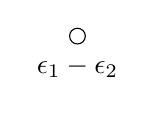
\begin{tikzpicture}
\draw[fill=white] (0 cm, 0 cm) circle (.1cm) node[below=4pt]{$\epsilon_{1} - \epsilon_{2}$};
\end{tikzpicture}
  \caption{The reduced hermitian symmetric pair $(\mathfrak{g}_\lambda, \mathfrak{k}_\lambda)$}
\end{figure}



\begin{figure}[H]
  \centering
      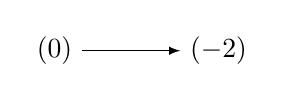
\begin{tikzpicture}[>=latex,line join=bevel,]
%%
\node (node_1) at (68.5bp,8.5bp) [draw,draw=none] {$\left(-2\right)$};
  \node (node_0) at (9.5bp,8.5bp) [draw,draw=none] {$\left(0\right)$};
  \draw [black,->] (node_0) ..controls (26.173bp,8.5bp) and (35.797bp,8.5bp)  .. (node_1);
%
\end{tikzpicture}
  \caption{Nilpotent cohomology / BGG resolution}
\end{figure}

        


\subsubsection{$\mathrm{SU}(1, 2)$: $ -\left(a_{2} + 2\right)\omega_{1} + \left(a_{2} + 1\right)\omega_{2} $}

The set of singular roots for the vertex: $\emptyset$ \\

\begin{figure}[H]
  \centering
  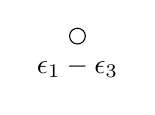
\begin{tikzpicture}
\draw[fill=white] (0 cm, 0 cm) circle (.1cm) node[below=4pt]{$\epsilon_{1} - \epsilon_{3}$};
\end{tikzpicture}
  \caption{The reduced hermitian symmetric pair $(\mathfrak{g}_\lambda, \mathfrak{k}_\lambda)$}
\end{figure}



\begin{figure}[H]
  \centering
      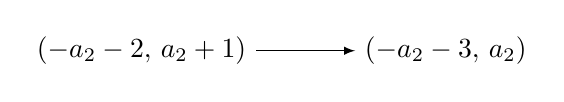
\begin{tikzpicture}[>=latex,line join=bevel,]
%%
\node (node_1) at (150.5bp,8.5bp) [draw,draw=none] {$\left(-a_{2} - 3,\,a_{2}\right)$};
  \node (node_0) at (41.0bp,8.5bp) [draw,draw=none] {$\left(-a_{2} - 2,\,a_{2} + 1\right)$};
  \draw [black,->] (node_0) ..controls (90.432bp,8.5bp) and (99.314bp,8.5bp)  .. (node_1);
%
\end{tikzpicture}
  \caption{Nilpotent cohomology / BGG resolution}
\end{figure}

        


\subsubsection{$\mathrm{SU}(1, 2)$: $ 0 $}

The set of singular roots for the vertex: $\emptyset$ \\

\begin{figure}[H]
  \centering
  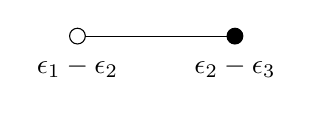
\begin{tikzpicture}
\draw (0 cm,0) -- (2 cm,0);
\draw[fill=white] (0 cm, 0 cm) circle (.1cm) node[below=4pt]{$\epsilon_{1} - \epsilon_{2}$};
\draw[fill=black] (2 cm, 0 cm) circle (.1cm) node[below=4pt]{$\epsilon_{2} - \epsilon_{3}$};
\end{tikzpicture}
  \caption{The reduced hermitian symmetric pair $(\mathfrak{g}_\lambda, \mathfrak{k}_\lambda)$}
\end{figure}



\begin{figure}[H]
  \centering
      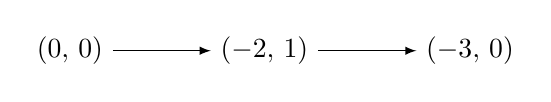
\begin{tikzpicture}[>=latex,line join=bevel,]
%%
\node (node_2) at (15.0bp,8.5bp) [draw,draw=none] {$\left(0,\,0\right)$};
  \node (node_1) at (85.0bp,8.5bp) [draw,draw=none] {$\left(-2,\,1\right)$};
  \node (node_0) at (159.0bp,8.5bp) [draw,draw=none] {$\left(-3,\,0\right)$};
  \draw [black,->] (node_2) ..controls (37.527bp,8.5bp) and (46.927bp,8.5bp)  .. (node_1);
  \draw [black,->] (node_1) ..controls (111.87bp,8.5bp) and (121.03bp,8.5bp)  .. (node_0);
%
\end{tikzpicture}
  \caption{Nilpotent cohomology / BGG resolution}
\end{figure}

        


\subsubsection{$\mathrm{SU}(1, 3)$: $ -\left(a_{2} + a_{3} + 3\right)\omega_{1} + \left(a_{3} + 1\right)\omega_{3} $}

The set of singular roots for the vertex: $\emptyset$ \\

\begin{figure}[H]
  \centering
  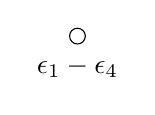
\begin{tikzpicture}
\draw[fill=white] (0 cm, 0 cm) circle (.1cm) node[below=4pt]{$\epsilon_{1} - \epsilon_{4}$};
\end{tikzpicture}
  \caption{The reduced hermitian symmetric pair $(\mathfrak{g}_\lambda, \mathfrak{k}_\lambda)$}
\end{figure}



\begin{figure}[H]
  \centering
      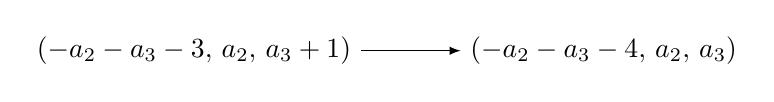
\begin{tikzpicture}[>=latex,line join=bevel,]
%%
\node (node_1) at (60.0bp,8.5bp) [draw,draw=none] {$\left(-a_{2} - a_{3} - 3,\,a_{2},\,a_{3} + 1\right)$};
  \node (node_0) at (207.5bp,8.5bp) [draw,draw=none] {$\left(-a_{2} - a_{3} - 4,\,a_{2},\,a_{3}\right)$};
  \draw [black,->] (node_1) ..controls (128.57bp,8.5bp) and (137.21bp,8.5bp)  .. (node_0);
%
\end{tikzpicture}
  \caption{Nilpotent cohomology / BGG resolution}
\end{figure}

        


\subsubsection{$\mathrm{SU}(1, 3)$: $ -\left(a_{2} + 2\right)\omega_{1} + \left(a_{2} + 1\right)\omega_{2} $}

The set of singular roots for the vertex: $\emptyset$ \\

\begin{figure}[H]
  \centering
  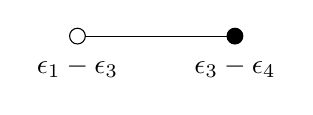
\begin{tikzpicture}
\draw (0 cm,0) -- (2 cm,0);
\draw[fill=white] (0 cm, 0 cm) circle (.1cm) node[below=4pt]{$\epsilon_{1} - \epsilon_{3}$};
\draw[fill=black] (2 cm, 0 cm) circle (.1cm) node[below=4pt]{$\epsilon_{3} - \epsilon_{4}$};
\end{tikzpicture}
  \caption{The reduced hermitian symmetric pair $(\mathfrak{g}_\lambda, \mathfrak{k}_\lambda)$}
\end{figure}



\begin{figure}[H]
  \centering
      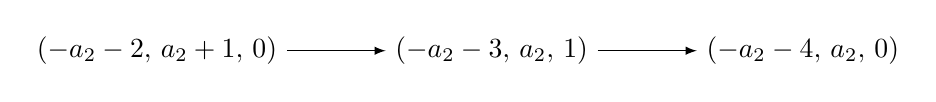
\begin{tikzpicture}[>=latex,line join=bevel,]
%%
\node (node_2) at (279.0bp,8.5bp) [draw,draw=none] {$\left(-a_{2} - 4,\,a_{2},\,0\right)$};
  \node (node_1) at (46.5bp,8.5bp) [draw,draw=none] {$\left(-a_{2} - 2,\,a_{2} + 1,\,0\right)$};
  \node (node_0) at (167.0bp,8.5bp) [draw,draw=none] {$\left(-a_{2} - 3,\,a_{2},\,1\right)$};
  \draw [black,->] (node_0) ..controls (213.39bp,8.5bp) and (222.13bp,8.5bp)  .. (node_2);
  \draw [black,->] (node_1) ..controls (101.65bp,8.5bp) and (110.36bp,8.5bp)  .. (node_0);
%
\end{tikzpicture}
  \caption{Nilpotent cohomology / BGG resolution}
\end{figure}

        


\subsubsection{$\mathrm{SU}(1, 3)$: $ 0 $}

The set of singular roots for the vertex: $\emptyset$ \\

\begin{figure}[H]
  \centering
  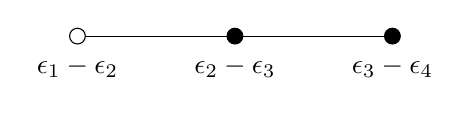
\begin{tikzpicture}
\draw (0 cm,0) -- (4 cm,0);
\draw[fill=white] (0 cm, 0 cm) circle (.1cm) node[below=4pt]{$\epsilon_{1} - \epsilon_{2}$};
\draw[fill=black] (2 cm, 0 cm) circle (.1cm) node[below=4pt]{$\epsilon_{2} - \epsilon_{3}$};
\draw[fill=black] (4 cm, 0 cm) circle (.1cm) node[below=4pt]{$\epsilon_{3} - \epsilon_{4}$};
\end{tikzpicture}
  \caption{The reduced hermitian symmetric pair $(\mathfrak{g}_\lambda, \mathfrak{k}_\lambda)$}
\end{figure}



\begin{figure}[H]
  \centering
      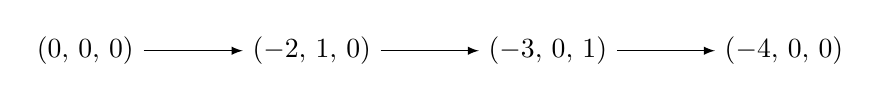
\begin{tikzpicture}[>=latex,line join=bevel,]
%%
\node (node_3) at (21.0bp,8.5bp) [draw,draw=none] {$\left(0,\,0,\,0\right)$};
  \node (node_2) at (102.5bp,8.5bp) [draw,draw=none] {$\left(-2,\,1,\,0\right)$};
  \node (node_1) at (187.5bp,8.5bp) [draw,draw=none] {$\left(-3,\,0,\,1\right)$};
  \node (node_0) at (272.5bp,8.5bp) [draw,draw=none] {$\left(-4,\,0,\,0\right)$};
  \draw [black,->] (node_2) ..controls (135.04bp,8.5bp) and (144.1bp,8.5bp)  .. (node_1);
  \draw [black,->] (node_3) ..controls (49.779bp,8.5bp) and (58.821bp,8.5bp)  .. (node_2);
  \draw [black,->] (node_1) ..controls (220.04bp,8.5bp) and (229.1bp,8.5bp)  .. (node_0);
%
\end{tikzpicture}
  \caption{Nilpotent cohomology / BGG resolution}
\end{figure}

        


\subsubsection{$\mathrm{SU}(2, 2)$: $ \left(a_{1} + 1\right)\omega_{1} - \left(a_{1} + a_{3} + 4\right)\omega_{2} + \left(a_{3} + 1\right)\omega_{3} $}

The set of singular roots for the vertex: $\emptyset$ \\

\begin{figure}[H]
  \centering
  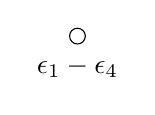
\begin{tikzpicture}
\draw[fill=white] (0 cm, 0 cm) circle (.1cm) node[below=4pt]{$\epsilon_{1} - \epsilon_{4}$};
\end{tikzpicture}
  \caption{The reduced hermitian symmetric pair $(\mathfrak{g}_\lambda, \mathfrak{k}_\lambda)$}
\end{figure}



\begin{figure}[H]
  \centering
      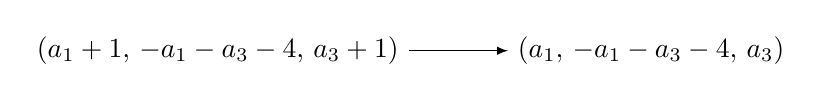
\begin{tikzpicture}[>=latex,line join=bevel,]
%%
\node (node_1) at (68.5bp,8.5bp) [draw,draw=none] {$\left(a_{1} + 1,\,-a_{1} - a_{3} - 4,\,a_{3} + 1\right)$};
  \node (node_0) at (224.5bp,8.5bp) [draw,draw=none] {$\left(a_{1},\,-a_{1} - a_{3} - 4,\,a_{3}\right)$};
  \draw [black,->] (node_1) ..controls (145.55bp,8.5bp) and (154.21bp,8.5bp)  .. (node_0);
%
\end{tikzpicture}
  \caption{Nilpotent cohomology / BGG resolution}
\end{figure}

        


\subsubsection{$\mathrm{SU}(2, 2)$: $ \left(a_{1} + 1\right)\omega_{1} - \left(a_{1} + 2\right)\omega_{2} $}

The set of singular roots for the vertex: $\{\epsilon_{2} - \epsilon_{4}$\} \\

\begin{figure}[H]
  \centering
  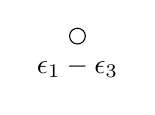
\begin{tikzpicture}
\draw[fill=white] (0 cm, 0 cm) circle (.1cm) node[below=4pt]{$\epsilon_{1} - \epsilon_{3}$};
\end{tikzpicture}
  \caption{The reduced hermitian symmetric pair $(\mathfrak{g}_\lambda, \mathfrak{k}_\lambda)$}
\end{figure}



\begin{figure}[H]
  \centering
      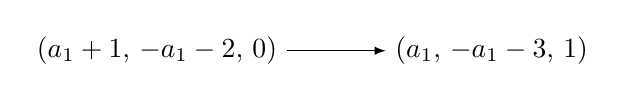
\begin{tikzpicture}[>=latex,line join=bevel,]
%%
\node (node_1) at (46.5bp,8.5bp) [draw,draw=none] {$\left(a_{1} + 1,\,-a_{1} - 2,\,0\right)$};
  \node (node_0) at (167.0bp,8.5bp) [draw,draw=none] {$\left(a_{1},\,-a_{1} - 3,\,1\right)$};
  \draw [black,->] (node_1) ..controls (101.65bp,8.5bp) and (110.36bp,8.5bp)  .. (node_0);
%
\end{tikzpicture}
  \caption{Nilpotent cohomology / BGG resolution}
\end{figure}

        


\subsubsection{$\mathrm{SU}(2, 2)$: $ -\left(a_{3} + 2\right)\omega_{2} + \left(a_{3} + 1\right)\omega_{3} $}

The set of singular roots for the vertex: $\{\epsilon_{1} - \epsilon_{3}$\} \\

\begin{figure}[H]
  \centering
  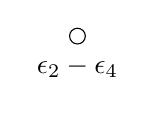
\begin{tikzpicture}
\draw[fill=white] (0 cm, 0 cm) circle (.1cm) node[below=4pt]{$\epsilon_{2} - \epsilon_{4}$};
\end{tikzpicture}
  \caption{The reduced hermitian symmetric pair $(\mathfrak{g}_\lambda, \mathfrak{k}_\lambda)$}
\end{figure}



\begin{figure}[H]
  \centering
      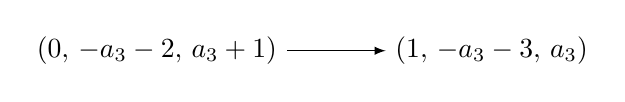
\begin{tikzpicture}[>=latex,line join=bevel,]
%%
\node (node_1) at (167.0bp,8.5bp) [draw,draw=none] {$\left(1,\,-a_{3} - 3,\,a_{3}\right)$};
  \node (node_0) at (46.5bp,8.5bp) [draw,draw=none] {$\left(0,\,-a_{3} - 2,\,a_{3} + 1\right)$};
  \draw [black,->] (node_0) ..controls (101.65bp,8.5bp) and (110.36bp,8.5bp)  .. (node_1);
%
\end{tikzpicture}
  \caption{Nilpotent cohomology / BGG resolution}
\end{figure}

        


\subsubsection{$\mathrm{SU}(2, 2)$: $ 0 $}

The set of singular roots for the vertex: $\emptyset$ \\

\begin{figure}[H]
  \centering
  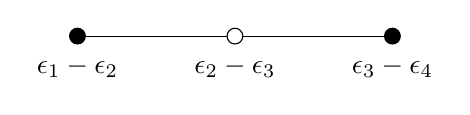
\begin{tikzpicture}
\draw (0 cm,0) -- (4 cm,0);
\draw[fill=black] (0 cm, 0 cm) circle (.1cm) node[below=4pt]{$\epsilon_{1} - \epsilon_{2}$};
\draw[fill=white] (2 cm, 0 cm) circle (.1cm) node[below=4pt]{$\epsilon_{2} - \epsilon_{3}$};
\draw[fill=black] (4 cm, 0 cm) circle (.1cm) node[below=4pt]{$\epsilon_{3} - \epsilon_{4}$};
\end{tikzpicture}
  \caption{The reduced hermitian symmetric pair $(\mathfrak{g}_\lambda, \mathfrak{k}_\lambda)$}
\end{figure}



\begin{figure}[H]
  \centering
      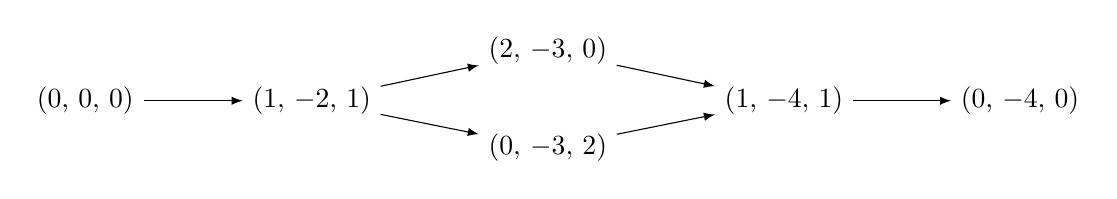
\begin{tikzpicture}[>=latex,line join=bevel,]
%%
\node (node_5) at (187.5bp,43.5bp) [draw,draw=none] {$\left(2,\,-3,\,0\right)$};
  \node (node_4) at (357.5bp,25.5bp) [draw,draw=none] {$\left(0,\,-4,\,0\right)$};
  \node (node_3) at (102.5bp,25.5bp) [draw,draw=none] {$\left(1,\,-2,\,1\right)$};
  \node (node_2) at (272.5bp,25.5bp) [draw,draw=none] {$\left(1,\,-4,\,1\right)$};
  \node (node_1) at (187.5bp,8.5bp) [draw,draw=none] {$\left(0,\,-3,\,2\right)$};
  \node (node_0) at (21.0bp,25.5bp) [draw,draw=none] {$\left(0,\,0,\,0\right)$};
  \draw [black,->] (node_0) ..controls (49.779bp,25.5bp) and (58.821bp,25.5bp)  .. (node_3);
  \draw [black,->] (node_3) ..controls (135.12bp,19.023bp) and (144.3bp,17.143bp)  .. (node_1);
  \draw [black,->] (node_5) ..controls (220.12bp,36.642bp) and (229.3bp,34.651bp)  .. (node_2);
  \draw [black,->] (node_1) ..controls (220.12bp,14.977bp) and (229.3bp,16.857bp)  .. (node_2);
  \draw [black,->] (node_3) ..controls (135.12bp,32.358bp) and (144.3bp,34.349bp)  .. (node_5);
  \draw [black,->] (node_2) ..controls (305.04bp,25.5bp) and (314.1bp,25.5bp)  .. (node_4);
%
\end{tikzpicture}
  \caption{Nilpotent cohomology / BGG resolution}
\end{figure}

        


\subsubsection{$\mathrm{SU}(2, 2)$: $ -\omega_{2} $}

The set of singular roots for the vertex: $\{\epsilon_{2} - \epsilon_{3}$\} \\

\begin{figure}[H]
  \centering
  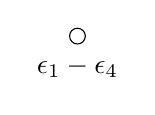
\begin{tikzpicture}
\draw[fill=white] (0 cm, 0 cm) circle (.1cm) node[below=4pt]{$\epsilon_{1} - \epsilon_{4}$};
\end{tikzpicture}
  \caption{The reduced hermitian symmetric pair $(\mathfrak{g}_\lambda, \mathfrak{k}_\lambda)$}
\end{figure}



\begin{figure}[H]
  \centering
      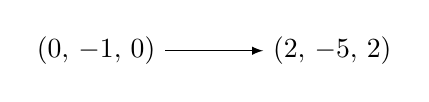
\begin{tikzpicture}[>=latex,line join=bevel,]
%%
\node (node_1) at (109.5bp,8.5bp) [draw,draw=none] {$\left(2,\,-5,\,2\right)$};
  \node (node_0) at (24.5bp,8.5bp) [draw,draw=none] {$\left(0,\,-1,\,0\right)$};
  \draw [black,->] (node_0) ..controls (57.035bp,8.5bp) and (66.102bp,8.5bp)  .. (node_1);
%
\end{tikzpicture}
  \caption{Nilpotent cohomology / BGG resolution}
\end{figure}

        


\subsubsection{$\mathrm{SU}(1, 4)$: $ -\left(a_{2} + a_{3} + a_{4} + 4\right)\omega_{1} + \left(a_{4} + 1\right)\omega_{4} $}

The set of singular roots for the vertex: $\emptyset$ \\

\begin{figure}[H]
  \centering
  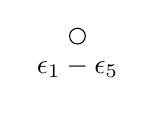
\begin{tikzpicture}
\draw[fill=white] (0 cm, 0 cm) circle (.1cm) node[below=4pt]{$\epsilon_{1} - \epsilon_{5}$};
\end{tikzpicture}
  \caption{The reduced hermitian symmetric pair $(\mathfrak{g}_\lambda, \mathfrak{k}_\lambda)$}
\end{figure}



\begin{figure}[H]
  \centering
      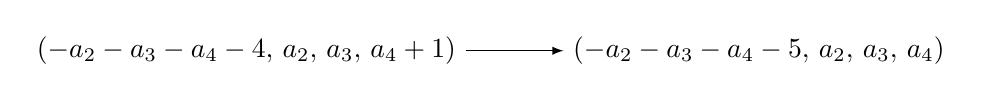
\begin{tikzpicture}[>=latex,line join=bevel,]
%%
\node (node_1) at (263.0bp,8.5bp) [draw,draw=none] {$\left(-a_{2} - a_{3} - a_{4} - 5,\,a_{2},\,a_{3},\,a_{4}\right)$};
  \node (node_0) at (78.5bp,8.5bp) [draw,draw=none] {$\left(-a_{2} - a_{3} - a_{4} - 4,\,a_{2},\,a_{3},\,a_{4} + 1\right)$};
  \draw [black,->] (node_0) ..controls (165.58bp,8.5bp) and (174.15bp,8.5bp)  .. (node_1);
%
\end{tikzpicture}
  \caption{Nilpotent cohomology / BGG resolution}
\end{figure}

        


\subsubsection{$\mathrm{SU}(1, 4)$: $ -\left(a_{2} + a_{3} + 3\right)\omega_{1} + \left(a_{3} + 1\right)\omega_{3} $}

The set of singular roots for the vertex: $\emptyset$ \\

\begin{figure}[H]
  \centering
  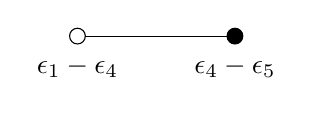
\begin{tikzpicture}
\draw (0 cm,0) -- (2 cm,0);
\draw[fill=white] (0 cm, 0 cm) circle (.1cm) node[below=4pt]{$\epsilon_{1} - \epsilon_{4}$};
\draw[fill=black] (2 cm, 0 cm) circle (.1cm) node[below=4pt]{$\epsilon_{4} - \epsilon_{5}$};
\end{tikzpicture}
  \caption{The reduced hermitian symmetric pair $(\mathfrak{g}_\lambda, \mathfrak{k}_\lambda)$}
\end{figure}



\begin{figure}[H]
  \centering
      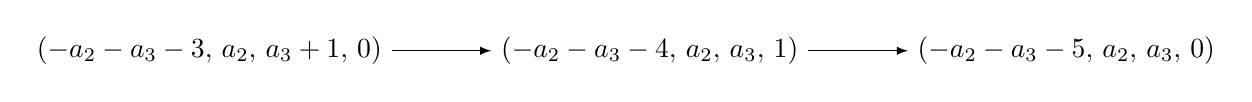
\begin{tikzpicture}[>=latex,line join=bevel,]
%%
\node (node_2) at (65.5bp,8.5bp) [draw,draw=none] {$\left(-a_{2} - a_{3} - 3,\,a_{2},\,a_{3} + 1,\,0\right)$};
  \node (node_1) at (224.0bp,8.5bp) [draw,draw=none] {$\left(-a_{2} - a_{3} - 4,\,a_{2},\,a_{3},\,1\right)$};
  \node (node_0) at (374.0bp,8.5bp) [draw,draw=none] {$\left(-a_{2} - a_{3} - 5,\,a_{2},\,a_{3},\,0\right)$};
  \draw [black,->] (node_2) ..controls (139.44bp,8.5bp) and (148.04bp,8.5bp)  .. (node_1);
  \draw [black,->] (node_1) ..controls (289.62bp,8.5bp) and (298.18bp,8.5bp)  .. (node_0);
%
\end{tikzpicture}
  \caption{Nilpotent cohomology / BGG resolution}
\end{figure}

        


\subsubsection{$\mathrm{SU}(1, 4)$: $ -\left(a_{2} + 2\right)\omega_{1} + \left(a_{2} + 1\right)\omega_{2} $}

The set of singular roots for the vertex: $\emptyset$ \\

\begin{figure}[H]
  \centering
  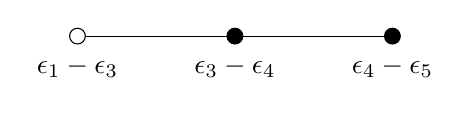
\begin{tikzpicture}
\draw (0 cm,0) -- (4 cm,0);
\draw[fill=white] (0 cm, 0 cm) circle (.1cm) node[below=4pt]{$\epsilon_{1} - \epsilon_{3}$};
\draw[fill=black] (2 cm, 0 cm) circle (.1cm) node[below=4pt]{$\epsilon_{3} - \epsilon_{4}$};
\draw[fill=black] (4 cm, 0 cm) circle (.1cm) node[below=4pt]{$\epsilon_{4} - \epsilon_{5}$};
\end{tikzpicture}
  \caption{The reduced hermitian symmetric pair $(\mathfrak{g}_\lambda, \mathfrak{k}_\lambda)$}
\end{figure}



\begin{figure}[H]
  \centering
      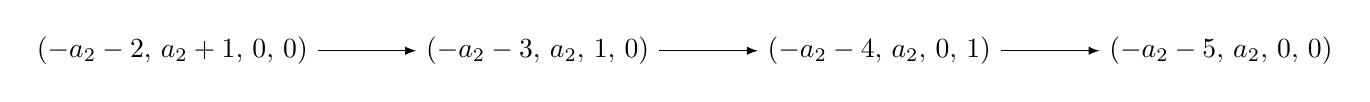
\begin{tikzpicture}[>=latex,line join=bevel,]
%%
\node (node_3) at (52.0bp,8.5bp) [draw,draw=none] {$\left(-a_{2} - 2,\,a_{2} + 1,\,0,\,0\right)$};
  \node (node_2) at (429.5bp,8.5bp) [draw,draw=none] {$\left(-a_{2} - 5,\,a_{2},\,0,\,0\right)$};
  \node (node_1) at (183.5bp,8.5bp) [draw,draw=none] {$\left(-a_{2} - 3,\,a_{2},\,1,\,0\right)$};
  \node (node_0) at (306.5bp,8.5bp) [draw,draw=none] {$\left(-a_{2} - 4,\,a_{2},\,0,\,1\right)$};
  \draw [black,->] (node_0) ..controls (358.38bp,8.5bp) and (367.09bp,8.5bp)  .. (node_2);
  \draw [black,->] (node_1) ..controls (235.38bp,8.5bp) and (244.09bp,8.5bp)  .. (node_0);
  \draw [black,->] (node_3) ..controls (112.53bp,8.5bp) and (121.18bp,8.5bp)  .. (node_1);
%
\end{tikzpicture}
  \caption{Nilpotent cohomology / BGG resolution}
\end{figure}

        


\subsubsection{$\mathrm{SU}(1, 4)$: $ 0 $}

The set of singular roots for the vertex: $\emptyset$ \\

\begin{figure}[H]
  \centering
  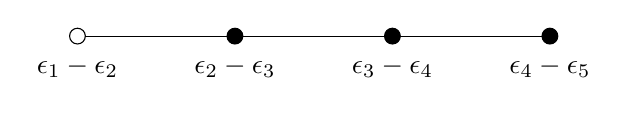
\begin{tikzpicture}
\draw (0 cm,0) -- (6 cm,0);
\draw[fill=white] (0 cm, 0 cm) circle (.1cm) node[below=4pt]{$\epsilon_{1} - \epsilon_{2}$};
\draw[fill=black] (2 cm, 0 cm) circle (.1cm) node[below=4pt]{$\epsilon_{2} - \epsilon_{3}$};
\draw[fill=black] (4 cm, 0 cm) circle (.1cm) node[below=4pt]{$\epsilon_{3} - \epsilon_{4}$};
\draw[fill=black] (6 cm, 0 cm) circle (.1cm) node[below=4pt]{$\epsilon_{4} - \epsilon_{5}$};
\end{tikzpicture}
  \caption{The reduced hermitian symmetric pair $(\mathfrak{g}_\lambda, \mathfrak{k}_\lambda)$}
\end{figure}



\begin{figure}[H]
  \centering
      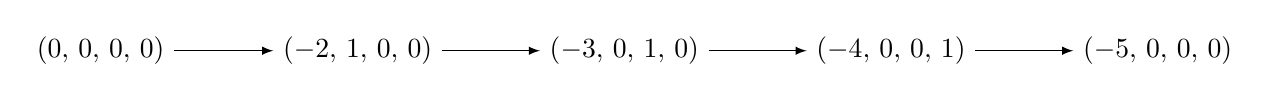
\begin{tikzpicture}[>=latex,line join=bevel,]
%%
\node (node_4) at (26.5bp,8.5bp) [draw,draw=none] {$\left(0,\,0,\,0,\,0\right)$};
  \node (node_3) at (311.0bp,8.5bp) [draw,draw=none] {$\left(-4,\,0,\,0,\,1\right)$};
  \node (node_2) at (407.0bp,8.5bp) [draw,draw=none] {$\left(-5,\,0,\,0,\,0\right)$};
  \node (node_1) at (119.0bp,8.5bp) [draw,draw=none] {$\left(-2,\,1,\,0,\,0\right)$};
  \node (node_0) at (215.0bp,8.5bp) [draw,draw=none] {$\left(-3,\,0,\,1,\,0\right)$};
  \draw [black,->] (node_3) ..controls (349.27bp,8.5bp) and (358.13bp,8.5bp)  .. (node_2);
  \draw [black,->] (node_0) ..controls (253.27bp,8.5bp) and (262.13bp,8.5bp)  .. (node_3);
  \draw [black,->] (node_1) ..controls (157.27bp,8.5bp) and (166.13bp,8.5bp)  .. (node_0);
  \draw [black,->] (node_4) ..controls (61.068bp,8.5bp) and (69.923bp,8.5bp)  .. (node_1);
%
\end{tikzpicture}
  \caption{Nilpotent cohomology / BGG resolution}
\end{figure}

        


\subsubsection{$\mathrm{SU}(2, 3)$: $ \left(a_{1} + 1\right)\omega_{1} - \left(a_{1} + a_{3} + a_{4} + 5\right)\omega_{2} + \left(a_{4} + 1\right)\omega_{4} $}

The set of singular roots for the vertex: $\emptyset$ \\

\begin{figure}[H]
  \centering
  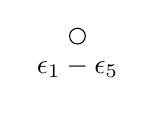
\begin{tikzpicture}
\draw[fill=white] (0 cm, 0 cm) circle (.1cm) node[below=4pt]{$\epsilon_{1} - \epsilon_{5}$};
\end{tikzpicture}
  \caption{The reduced hermitian symmetric pair $(\mathfrak{g}_\lambda, \mathfrak{k}_\lambda)$}
\end{figure}



\begin{figure}[H]
  \centering
      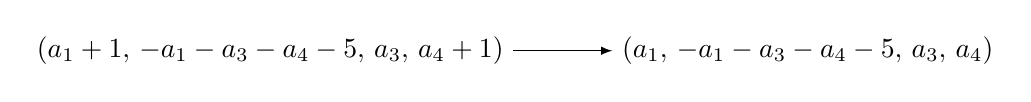
\begin{tikzpicture}[>=latex,line join=bevel,]
%%
\node (node_1) at (281.0bp,8.5bp) [draw,draw=none] {$\left(a_{1},\,-a_{1} - a_{3} - a_{4} - 5,\,a_{3},\,a_{4}\right)$};
  \node (node_0) at (87.5bp,8.5bp) [draw,draw=none] {$\left(a_{1} + 1,\,-a_{1} - a_{3} - a_{4} - 5,\,a_{3},\,a_{4} + 1\right)$};
  \draw [black,->] (node_0) ..controls (183.53bp,8.5bp) and (192.16bp,8.5bp)  .. (node_1);
%
\end{tikzpicture}
  \caption{Nilpotent cohomology / BGG resolution}
\end{figure}

        


\subsubsection{$\mathrm{SU}(2, 3)$: $ \left(a_{1} + 1\right)\omega_{1} - \left(a_{1} + a_{3} + 4\right)\omega_{2} + \left(a_{3} + 1\right)\omega_{3} $}

The set of singular roots for the vertex: $\{\epsilon_{2} - \epsilon_{5}$\} \\

\begin{figure}[H]
  \centering
  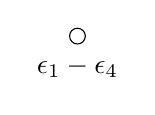
\begin{tikzpicture}
\draw[fill=white] (0 cm, 0 cm) circle (.1cm) node[below=4pt]{$\epsilon_{1} - \epsilon_{4}$};
\end{tikzpicture}
  \caption{The reduced hermitian symmetric pair $(\mathfrak{g}_\lambda, \mathfrak{k}_\lambda)$}
\end{figure}



\begin{figure}[H]
  \centering
      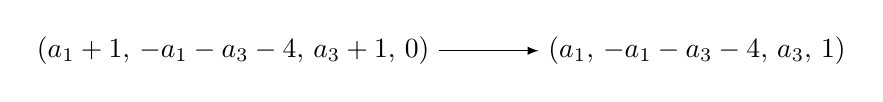
\begin{tikzpicture}[>=latex,line join=bevel,]
%%
\node (node_1) at (74.0bp,8.5bp) [draw,draw=none] {$\left(a_{1} + 1,\,-a_{1} - a_{3} - 4,\,a_{3} + 1,\,0\right)$};
  \node (node_0) at (241.0bp,8.5bp) [draw,draw=none] {$\left(a_{1},\,-a_{1} - a_{3} - 4,\,a_{3},\,1\right)$};
  \draw [black,->] (node_1) ..controls (156.78bp,8.5bp) and (165.35bp,8.5bp)  .. (node_0);
%
\end{tikzpicture}
  \caption{Nilpotent cohomology / BGG resolution}
\end{figure}

        


\subsubsection{$\mathrm{SU}(2, 3)$: $ \left(a_{1} + 1\right)\omega_{1} - \left(a_{1} + 2\right)\omega_{2} $}

The set of singular roots for the vertex: $\{\epsilon_{2} - \epsilon_{4}$\} \\

\begin{figure}[H]
  \centering
  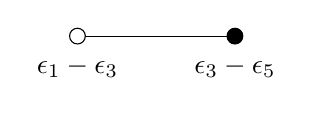
\begin{tikzpicture}
\draw (0 cm,0) -- (2 cm,0);
\draw[fill=white] (0 cm, 0 cm) circle (.1cm) node[below=4pt]{$\epsilon_{1} - \epsilon_{3}$};
\draw[fill=black] (2 cm, 0 cm) circle (.1cm) node[below=4pt]{$\epsilon_{3} - \epsilon_{5}$};
\end{tikzpicture}
  \caption{The reduced hermitian symmetric pair $(\mathfrak{g}_\lambda, \mathfrak{k}_\lambda)$}
\end{figure}



\begin{figure}[H]
  \centering
      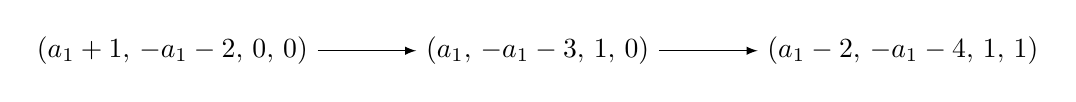
\begin{tikzpicture}[>=latex,line join=bevel,]
%%
\node (node_2) at (315.0bp,8.5bp) [draw,draw=none] {$\left(a_{1} - 2,\,-a_{1} - 4,\,1,\,1\right)$};
  \node (node_1) at (52.0bp,8.5bp) [draw,draw=none] {$\left(a_{1} + 1,\,-a_{1} - 2,\,0,\,0\right)$};
  \node (node_0) at (183.5bp,8.5bp) [draw,draw=none] {$\left(a_{1},\,-a_{1} - 3,\,1,\,0\right)$};
  \draw [black,->] (node_0) ..controls (235.42bp,8.5bp) and (244.1bp,8.5bp)  .. (node_2);
  \draw [black,->] (node_1) ..controls (112.53bp,8.5bp) and (121.18bp,8.5bp)  .. (node_0);
%
\end{tikzpicture}
  \caption{Nilpotent cohomology / BGG resolution}
\end{figure}

        


\subsubsection{$\mathrm{SU}(2, 3)$: $ -\left(a_{3} + a_{4} + 3\right)\omega_{2} + \left(a_{4} + 1\right)\omega_{4} $}

The set of singular roots for the vertex: $\{\epsilon_{1} - \epsilon_{4}$\} \\

\begin{figure}[H]
  \centering
  \begin{tikzpicture}
\draw[fill=white] (0 cm, 0 cm) circle (.1cm) node[below=4pt]{$\epsilon_{2} - \epsilon_{5}$};
\end{tikzpicture}
  \caption{The reduced hermitian symmetric pair $(\mathfrak{g}_\lambda, \mathfrak{k}_\lambda)$}
\end{figure}



\begin{figure}[H]
  \centering
      \begin{tikzpicture}[>=latex,line join=bevel,]
%%
\node (node_1) at (65.5bp,8.5bp) [draw,draw=none] {$\left(0,\,-a_{3} - a_{4} - 3,\,a_{3},\,a_{4} + 1\right)$};
  \node (node_0) at (224.0bp,8.5bp) [draw,draw=none] {$\left(1,\,-a_{3} - a_{4} - 4,\,a_{3},\,a_{4}\right)$};
  \draw [black,->] (node_1) ..controls (139.44bp,8.5bp) and (148.04bp,8.5bp)  .. (node_0);
%
\end{tikzpicture}
  \caption{Nilpotent cohomology / BGG resolution}
\end{figure}

        


\subsubsection{$\mathrm{SU}(2, 3)$: $ -\left(a_{3} + 2\right)\omega_{2} + \left(a_{3} + 1\right)\omega_{3} $}

The set of singular roots for the vertex: $\{\epsilon_{1} - \epsilon_{3}$\} \\

\begin{figure}[H]
  \centering
  \begin{tikzpicture}
\draw (0 cm,0) -- (2 cm,0);
\draw[fill=white] (0 cm, 0 cm) circle (.1cm) node[below=4pt]{$\epsilon_{2} - \epsilon_{4}$};
\draw[fill=black] (2 cm, 0 cm) circle (.1cm) node[below=4pt]{$\epsilon_{4} - \epsilon_{5}$};
\end{tikzpicture}
  \caption{The reduced hermitian symmetric pair $(\mathfrak{g}_\lambda, \mathfrak{k}_\lambda)$}
\end{figure}



\begin{figure}[H]
  \centering
      \begin{tikzpicture}[>=latex,line join=bevel,]
%%
\node (node_2) at (306.5bp,8.5bp) [draw,draw=none] {$\left(2,\,-a_{3} - 4,\,a_{3},\,0\right)$};
  \node (node_1) at (52.0bp,8.5bp) [draw,draw=none] {$\left(0,\,-a_{3} - 2,\,a_{3} + 1,\,0\right)$};
  \node (node_0) at (183.5bp,8.5bp) [draw,draw=none] {$\left(1,\,-a_{3} - 3,\,a_{3},\,1\right)$};
  \draw [black,->] (node_0) ..controls (235.38bp,8.5bp) and (244.09bp,8.5bp)  .. (node_2);
  \draw [black,->] (node_1) ..controls (112.53bp,8.5bp) and (121.18bp,8.5bp)  .. (node_0);
%
\end{tikzpicture}
  \caption{Nilpotent cohomology / BGG resolution}
\end{figure}

        


\subsubsection{$\mathrm{SU}(2, 3)$: $ -\left(a_{3} + 3\right)\omega_{2} + \left(a_{3} + 1\right)\omega_{3} $}

The set of singular roots for the vertex: $\{\epsilon_{2} - \epsilon_{4}$\} \\

\begin{figure}[H]
  \centering
  \begin{tikzpicture}
\draw[fill=white] (0 cm, 0 cm) circle (.1cm) node[below=4pt]{$\epsilon_{1} - \epsilon_{5}$};
\end{tikzpicture}
  \caption{The reduced hermitian symmetric pair $(\mathfrak{g}_\lambda, \mathfrak{k}_\lambda)$}
\end{figure}



\begin{figure}[H]
  \centering
      \begin{tikzpicture}[>=latex,line join=bevel,]
%%
\node (node_1) at (52.0bp,8.5bp) [draw,draw=none] {$\left(0,\,-a_{3} - 3,\,a_{3} + 1,\,0\right)$};
  \node (node_0) at (192.0bp,8.5bp) [draw,draw=none] {$\left(2,\,-a_{3} - 5,\,a_{3} - 1,\,2\right)$};
  \draw [black,->] (node_1) ..controls (112.56bp,8.5bp) and (121.08bp,8.5bp)  .. (node_0);
%
\end{tikzpicture}
  \caption{Nilpotent cohomology / BGG resolution}
\end{figure}

        


\subsubsection{$\mathrm{SU}(2, 3)$: $ 0 $}

The set of singular roots for the vertex: $\emptyset$ \\

\begin{figure}[H]
  \centering
  \begin{tikzpicture}
\draw (0 cm,0) -- (6 cm,0);
\draw[fill=black] (0 cm, 0 cm) circle (.1cm) node[below=4pt]{$\epsilon_{1} - \epsilon_{2}$};
\draw[fill=white] (2 cm, 0 cm) circle (.1cm) node[below=4pt]{$\epsilon_{2} - \epsilon_{3}$};
\draw[fill=black] (4 cm, 0 cm) circle (.1cm) node[below=4pt]{$\epsilon_{3} - \epsilon_{4}$};
\draw[fill=black] (6 cm, 0 cm) circle (.1cm) node[below=4pt]{$\epsilon_{4} - \epsilon_{5}$};
\end{tikzpicture}
  \caption{The reduced hermitian symmetric pair $(\mathfrak{g}_\lambda, \mathfrak{k}_\lambda)$}
\end{figure}



\begin{figure}[H]
  \centering
      \begin{tikzpicture}[>=latex,line join=bevel,]
%%
\node (node_9) at (311.0bp,43.5bp) [draw,draw=none] {$\left(3,\,-4,\,0,\,0\right)$};
  \node (node_8) at (26.5bp,25.5bp) [draw,draw=none] {$\left(0,\,0,\,0,\,0\right)$};
  \node (node_7) at (119.0bp,25.5bp) [draw,draw=none] {$\left(1,\,-2,\,1,\,0\right)$};
  \node (node_6) at (407.0bp,43.5bp) [draw,draw=none] {$\left(2,\,-5,\,1,\,0\right)$};
  \node (node_5) at (311.0bp,8.5bp) [draw,draw=none] {$\left(1,\,-4,\,1,\,1\right)$};
  \node (node_4) at (215.0bp,8.5bp) [draw,draw=none] {$\left(0,\,-3,\,2,\,0\right)$};
  \node (node_3) at (407.0bp,8.5bp) [draw,draw=none] {$\left(0,\,-4,\,0,\,2\right)$};
  \node (node_2) at (599.0bp,25.5bp) [draw,draw=none] {$\left(0,\,-5,\,0,\,0\right)$};
  \node (node_1) at (503.0bp,25.5bp) [draw,draw=none] {$\left(1,\,-5,\,0,\,1\right)$};
  \node (node_0) at (215.0bp,43.5bp) [draw,draw=none] {$\left(2,\,-3,\,0,\,1\right)$};
  \draw [black,->] (node_4) ..controls (253.27bp,8.5bp) and (262.13bp,8.5bp)  .. (node_5);
  \draw [black,->] (node_5) ..controls (346.73bp,21.432bp) and (360.8bp,26.672bp)  .. (node_6);
  \draw [black,->] (node_6) ..controls (445.36bp,36.346bp) and (454.33bp,34.628bp)  .. (node_1);
  \draw [black,->] (node_3) ..controls (445.36bp,15.257bp) and (454.33bp,16.879bp)  .. (node_1);
  \draw [black,->] (node_7) ..controls (157.36bp,18.743bp) and (166.33bp,17.121bp)  .. (node_4);
  \draw [black,->] (node_9) ..controls (349.27bp,43.5bp) and (358.13bp,43.5bp)  .. (node_6);
  \draw [black,->] (node_0) ..controls (250.73bp,30.568bp) and (264.8bp,25.328bp)  .. (node_5);
  \draw [black,->] (node_5) ..controls (349.27bp,8.5bp) and (358.13bp,8.5bp)  .. (node_3);
  \draw [black,->] (node_0) ..controls (253.27bp,43.5bp) and (262.13bp,43.5bp)  .. (node_9);
  \draw [black,->] (node_1) ..controls (541.27bp,25.5bp) and (550.13bp,25.5bp)  .. (node_2);
  \draw [black,->] (node_8) ..controls (61.068bp,25.5bp) and (69.923bp,25.5bp)  .. (node_7);
  \draw [black,->] (node_7) ..controls (157.36bp,32.654bp) and (166.33bp,34.372bp)  .. (node_0);
%
\end{tikzpicture}
  \caption{Nilpotent cohomology / BGG resolution}
\end{figure}

        


\subsubsection{$\mathrm{SU}(2, 3)$: $ -\omega_{2} $}

The set of singular roots for the vertex: $\{\epsilon_{2} - \epsilon_{3}$\} \\

\begin{figure}[H]
  \centering
  \begin{tikzpicture}
\draw (0 cm,0) -- (2 cm,0);
\draw[fill=white] (0 cm, 0 cm) circle (.1cm) node[below=4pt]{$\epsilon_{1} - \epsilon_{4}$};
\draw[fill=black] (2 cm, 0 cm) circle (.1cm) node[below=4pt]{$\epsilon_{4} - \epsilon_{5}$};
\end{tikzpicture}
  \caption{The reduced hermitian symmetric pair $(\mathfrak{g}_\lambda, \mathfrak{k}_\lambda)$}
\end{figure}



\begin{figure}[H]
  \centering
      \begin{tikzpicture}[>=latex,line join=bevel,]
%%
\node (node_2) at (222.0bp,8.5bp) [draw,draw=none] {$\left(3,\,-6,\,1,\,1\right)$};
  \node (node_1) at (126.0bp,8.5bp) [draw,draw=none] {$\left(2,\,-5,\,2,\,0\right)$};
  \node (node_0) at (30.0bp,8.5bp) [draw,draw=none] {$\left(0,\,-1,\,0,\,0\right)$};
  \draw [black,->] (node_0) ..controls (68.273bp,8.5bp) and (77.134bp,8.5bp)  .. (node_1);
  \draw [black,->] (node_1) ..controls (164.27bp,8.5bp) and (173.13bp,8.5bp)  .. (node_2);
%
\end{tikzpicture}
  \caption{Nilpotent cohomology / BGG resolution}
\end{figure}

\clearpage


\subsection[Sp(n,R)]{$\mathrm{Sp}(n,\R) \sim C_n, n \geq 2$}

\subsubsection{Root system data}

\[ \alpha_i = \epsilon_i - \epsilon_{i+1}, i< n,a_n = 2\epsilon_n, \quad \omega_i=\epsilon_1+\cdots+\epsilon_i\]
\begin{align*}
 \roots &= \{\pm \epsilon_i \pm \epsilon_j | i,j = 1,\ldots, n \}\setminus\{0\}\\
 \roots_c^+ &= \{ \epsilon_i-\epsilon_j | 1\leq i < j \leq  n\}\\
 \roots_n^+ &= \{ \epsilon_i + \epsilon_j | 1 \leq i \leq  j \leq n \}
\end{align*}
\[\beta = 2\epsilon_1,\quad \rho = (n,\ldots ,1),\quad \zeta = (1,1,\ldots,1)\]
\inserttikzfigure{diagrams/dynkin_Cn_n.tikz}{Marked Dynkin diagram of $\mathrm{Sp}(n,\R)$}

The reduction points of unitarizable highest weight modules are the following integral translated cones $\lambda_a + C_a$:
Let $a=(Q,R,l)$, $R=\mathrm{Sp}(r,\R)$ and $1\leq l \leq r \leq n$. Then
\[
 C_a = \{ a_r\omega_r + \cdots + a_n\omega_n \,|\, a_n=-(a_r+\cdots + a_{n-1}) \}
\]
and
\begin{gather*}
  \lambda_a = \omega_q + \omega_r - (2+n-\frac{1}{2}(r+q-l+1))\omega_n\\
  \mu_a= \omega_{q-l} + \omega_{r-l} - (2+n-\frac{1}{2}(r+q-l+1))\omega_n\\
   1\leq q\leq r\leq n,\quad 1\leq l \leq q\\
   Q(\lambda_a) = \mathrm{Sp}(q,\R),\quad R(\lambda_a)= \mathrm{Sp}(r,\R)
\end{gather*}

\subsubsection{Nilpotent cohomology in detail}

Scalar products of $\rho$ with noncompact roots
\begin{align*}
 (\epsilon_i - \epsilon_j, \rho ) & = n-i+1 - (n-j+1) = j - i \\
 (\epsilon_i + \epsilon_j, \rho ) & = n-i+1 + (n-j+1) = 2n+2-i-j.
\end{align*}


The $i$th coordinate of $\lambda$ with respect to the $\epsilon$-basis is
\[
 (\epsilon_i, \lambda) = \begin{cases}
                          2+ \frac{1}{2}(r+q-l+1) - n -2, & 1\leq i \leq q \\
                          1 + \frac{1}{2}(r+q-l+1) - n -2,  & q < i \leq r \\
                          \frac{1}{2}(r+q-l+1) - n -2,  & r < i.
                         \end{cases}
\]
Computation of $(\epsilon_i - \epsilon_j, \lambda + \rho)$ for $j > i$ leads to the following table
\begin{center}
\begin{tabular}{C|CCC}
                  & 1 < j \leq q & q < j \leq r & r < j \leq n \\[2pt]\hline
   1\leq i \leq q & j - i        & 1+j-i        & 2+j-i        \\
  q < i \leq r    &              & j-i		& 1+j-i        \\
  r < i \leq n	  & 		 & 		& j-i	
\end{tabular}
\end{center}
and  scalar products of the remaining positive roots $\epsilon_i + \epsilon_j$, $j\geq i$ are
\begin{center}
\begin{tabular}{C|CCC}
                  & 1 < j \leq q & q < j \leq r & r < j \leq n \\[2pt]\hline
   1\leq i \leq q & 3+m-i-j      & 2 + m -i-j   & 1 + m  -i-j      \\
  q < i \leq r    &              & 1 + m-i-j	& m    -i-j    \\
  r < i \leq n	  & 		 & 		& m-1-i-j
\end{tabular}
\end{center}
where
\[
 m = r+q-l.
\]
We see again that only noncompact roots can be orthogonal to $\lambda+\rho$ in accordance with the lemma \ref{lem:singular_are_noncompact}. If a positive noncompact root $\epsilon_i + \epsilon_j$ belongs to $\Psi^+_\lambda$, then
\begin{enumerate}
  \item $1\leq i \leq q$
    \begin{enumerate}
      \item $1 \leq j \leq q$: \[ 3+r-l \leq i \leq \min \left\{ q, \frac{3+m}{2} \right \}\]
      \item $q < j \leq r$: \[ 2+q-l \leq i \leq \min \{ 1+r-l, q \}  \]
      \item $r < j \leq n$: \[ \max \{ 1, 1+m-n \} \leq i \leq q-l  \]
    \end{enumerate}
  \item $q <  i \leq r$
    \begin{enumerate}
      \item $q < j \leq r$: \[  1+q \leq i \leq \frac{1+m}{2} \]
      \item $r < j \leq n$: \[ m-n \leq i < q-l \]
    \end{enumerate}
  \item $r < i \leq n$, \quad $r < j \leq n$: \[ \max \{ r+1,  m-n-1 \} \leq i \leq \frac{m-1}{2}. \]
\end{enumerate}
The set of indices 2a is empty, because $q-l < q$; similarly the third set is empty since $r+1 > \frac{m-1}{2}$.

A singular long root exists if and only if
\[
  m \text{ is odd and } (3+r \leq q+l \text{ or } q+l < 1+r)
\]
or alternatively a singular root doesn't exist if and only if
\[
 m \text{ is even or } m \text{ is odd and either } q+l = 2+r \text{ or } q+l = 1+r.
\]


Two positive noncompact roots are orthogonal if and only if the intersection of their indices is empty, i.e.
\[
 (\epsilon_i + \epsilon_j,\epsilon_k + \epsilon_l) = 0 \Longleftrightarrow \{i,j\} \cap \{k,l\} = \emptyset.
\]


\begin{figure}[H]
  \centering 
  \resizebox{\textwidth}{!}{%
	\begin{tikzpicture}[>=latex,line join=bevel,]
%%
\node (alpha3+2*alpha4+alpha5) at (89bp,268bp) [draw,draw=none] {$\alpha_{3} + 2\alpha_{4} + \alpha_{5}$};
  \node (alpha1+alpha2+2*alpha3+2*alpha4+alpha5) at (208bp,112bp) [draw,draw=none] {$\alpha_{1} + \alpha_{2} + 2\alpha_{3} + 2\alpha_{4} + \alpha_{5}$};
  \node (alpha5) at (125bp,420bp) [draw,draw=none] {$\alpha_{5}$};
  \node (2*alpha2+2*alpha3+2*alpha4+alpha5) at (79bp,112bp) [draw,draw=none] {$2\alpha_{2} + 2\alpha_{3} + 2\alpha_{4} + \alpha_{5}$};
  \node (alpha1+alpha2+alpha3+2*alpha4+alpha5) at (208bp,164bp) [draw,draw=none] {$\alpha_{1} + \alpha_{2} + \alpha_{3} + 2\alpha_{4} + \alpha_{5}$};
  \node (2*alpha1+2*alpha2+2*alpha3+2*alpha4+alpha5) at (143bp,8bp) [draw,draw=none] {$2\alpha_{1} + 2\alpha_{2} + 2\alpha_{3} + 2\alpha_{4} + \alpha_{5}$};
  \node (alpha2+alpha3+2*alpha4+alpha5) at (137bp,216bp) [draw,draw=none] {$\alpha_{2} + \alpha_{3} + 2\alpha_{4} + \alpha_{5}$};
  \node (alpha2+alpha3+alpha4+alpha5) at (185bp,268bp) [draw,draw=none] {$\alpha_{2} + \alpha_{3} + \alpha_{4} + \alpha_{5}$};
  \node (alpha4+alpha5) at (125bp,371bp) [draw,draw=none] {$\alpha_{4} + \alpha_{5}$};
  \node (2*alpha3+2*alpha4+alpha5) at (36bp,216bp) [draw,draw=none] {$2\alpha_{3} + 2\alpha_{4} + \alpha_{5}$};
  \node (alpha1+2*alpha2+2*alpha3+2*alpha4+alpha5) at (143bp,60bp) [draw,draw=none] {$\alpha_{1} + 2\alpha_{2} + 2\alpha_{3} + 2\alpha_{4} + \alpha_{5}$};
  \node (alpha2+2*alpha3+2*alpha4+alpha5) at (81bp,164bp) [draw,draw=none] {$\alpha_{2} + 2\alpha_{3} + 2\alpha_{4} + \alpha_{5}$};
  \node (alpha1+alpha2+alpha3+alpha4+alpha5) at (256bp,216bp) [draw,draw=none] {$\alpha_{1} + \alpha_{2} + \alpha_{3} + \alpha_{4} + \alpha_{5}$};
  \node (2*alpha4+alpha5) at (89bp,320bp) [draw,draw=none] {$2\alpha_{4} + \alpha_{5}$};
  \node (alpha3+alpha4+alpha5) at (162bp,320bp) [draw,draw=none] {$\alpha_{3} + \alpha_{4} + \alpha_{5}$};
  \draw [black,->] (alpha2+2*alpha3+2*alpha4+alpha5) ..controls (119.09bp,148bp) and (156.76bp,133.17bp)  .. (alpha1+alpha2+2*alpha3+2*alpha4+alpha5);
  \draw [black,->] (alpha3+2*alpha4+alpha5) ..controls (74.101bp,252.94bp) and (60.793bp,240.39bp)  .. (2*alpha3+2*alpha4+alpha5);
  \draw [black,->] (alpha2+alpha3+alpha4+alpha5) ..controls (204.88bp,253bp) and (224.54bp,239.16bp)  .. (alpha1+alpha2+alpha3+alpha4+alpha5);
  \draw [black,->] (alpha3+alpha4+alpha5) ..controls (168.06bp,305.82bp) and (173.5bp,293.99bp)  .. (alpha2+alpha3+alpha4+alpha5);
  \draw [black,->] (alpha4+alpha5) ..controls (115.46bp,357.02bp) and (106.83bp,345.27bp)  .. (2*alpha4+alpha5);
  \draw [black,->] (alpha5) ..controls (125bp,407.84bp) and (125bp,397.19bp)  .. (alpha4+alpha5);
  \draw [black,->] (alpha1+alpha2+alpha3+2*alpha4+alpha5) ..controls (208bp,149.76bp) and (208bp,139.06bp)  .. (alpha1+alpha2+2*alpha3+2*alpha4+alpha5);
  \draw [black,->] (alpha3+alpha4+alpha5) ..controls (141.7bp,305.09bp) and (121.85bp,291.5bp)  .. (alpha3+2*alpha4+alpha5);
  \draw [black,->] (alpha1+alpha2+alpha3+alpha4+alpha5) ..controls (243.07bp,201.53bp) and (231.06bp,189.02bp)  .. (alpha1+alpha2+alpha3+2*alpha4+alpha5);
  \draw [black,->] (alpha4+alpha5) ..controls (134.92bp,356.86bp) and (144.07bp,344.75bp)  .. (alpha3+alpha4+alpha5);
  \draw [black,->] (2*alpha3+2*alpha4+alpha5) ..controls (48.516bp,201.09bp) and (59.504bp,188.88bp)  .. (alpha2+2*alpha3+2*alpha4+alpha5);
  \draw [black,->] (alpha3+2*alpha4+alpha5) ..controls (102.42bp,253.02bp) and (114.31bp,240.64bp)  .. (alpha2+alpha3+2*alpha4+alpha5);
  \draw [black,->] (2*alpha2+2*alpha3+2*alpha4+alpha5) ..controls (97.182bp,96.795bp) and (113.7bp,83.89bp)  .. (alpha1+2*alpha2+2*alpha3+2*alpha4+alpha5);
  \draw [black,->] (alpha1+2*alpha2+2*alpha3+2*alpha4+alpha5) ..controls (143bp,45.763bp) and (143bp,35.065bp)  .. (2*alpha1+2*alpha2+2*alpha3+2*alpha4+alpha5);
  \draw [black,->] (2*alpha4+alpha5) ..controls (89bp,305.76bp) and (89bp,295.06bp)  .. (alpha3+2*alpha4+alpha5);
  \draw [black,->] (alpha2+2*alpha3+2*alpha4+alpha5) ..controls (80.471bp,149.76bp) and (80.043bp,139.06bp)  .. (2*alpha2+2*alpha3+2*alpha4+alpha5);
  \draw [black,->] (alpha1+alpha2+2*alpha3+2*alpha4+alpha5) ..controls (189.44bp,96.721bp) and (172.43bp,83.639bp)  .. (alpha1+2*alpha2+2*alpha3+2*alpha4+alpha5);
  \draw [black,->] (alpha2+alpha3+2*alpha4+alpha5) ..controls (157.38bp,200.65bp) and (176.21bp,187.39bp)  .. (alpha1+alpha2+alpha3+2*alpha4+alpha5);
  \draw [black,->] (alpha2+alpha3+2*alpha4+alpha5) ..controls (121.17bp,200.87bp) and (106.92bp,188.14bp)  .. (alpha2+2*alpha3+2*alpha4+alpha5);
  \draw [black,->] (alpha2+alpha3+alpha4+alpha5) ..controls (172.07bp,253.53bp) and (160.06bp,241.02bp)  .. (alpha2+alpha3+2*alpha4+alpha5);
%
\end{tikzpicture}
	\begin{tikzpicture}[>=latex,line join=bevel,]
%%
\node (s5*s4*s5*s3*s4*s5*s2*s1) at (174bp,342bp) [draw,draw=none] {$s_{5}s_{4}s_{5}s_{3}s_{4}s_{5}s_{2}s_{1}$};
  \node (s5*s4*s5*s3*s4*s5*s2*s3*s4*s5*s1*s2) at (102bp,150bp) [draw,draw=none] {$s_{5}s_{4}s_{5}s_{3}s_{4}s_{5}s_{2}s_{3}s_{4}s_{5}s_{1}s_{2}$};
  \node (s5*s4*s5*s3*s4*s5*s2*s3*s4*s5*s1*s2*s3*s4*s5) at (169bp,6bp) [draw,draw=none] {$s_{5}s_{4}s_{5}s_{3}s_{4}s_{5}s_{2}s_{3}s_{4}s_{5}s_{1}s_{2}s_{3}s_{4}s_{5}$};
  \node (s5*s4*s5*s3*s4*s5*s2*s3*s4*s5*s1*s2*s3) at (169bp,102bp) [draw,draw=none] {$s_{5}s_{4}s_{5}s_{3}s_{4}s_{5}s_{2}s_{3}s_{4}s_{5}s_{1}s_{2}s_{3}$};
  \node (s5*s4) at (183bp,630bp) [draw,draw=none] {$s_{5}s_{4}$};
  \node (1) at (183bp,727bp) [draw,draw=none] {$1$};
  \node (s5*s4*s5*s3*s4*s5*s2*s3*s4) at (67bp,294bp) [draw,draw=none] {$s_{5}s_{4}s_{5}s_{3}s_{4}s_{5}s_{2}s_{3}s_{4}$};
  \node (s5*s4*s5*s3*s4*s5*s2*s3*s4*s5*s1*s2*s3*s4) at (169bp,54bp) [draw,draw=none] {$s_{5}s_{4}s_{5}s_{3}s_{4}s_{5}s_{2}s_{3}s_{4}s_{5}s_{1}s_{2}s_{3}s_{4}$};
  \node (s5*s4*s5*s3*s4*s5*s2*s3*s4*s1*s2*s3) at (236bp,150bp) [draw,draw=none] {$s_{5}s_{4}s_{5}s_{3}s_{4}s_{5}s_{2}s_{3}s_{4}s_{1}s_{2}s_{3}$};
  \node (s5*s4*s5*s3*s4*s5*s2*s3*s1) at (174bp,294bp) [draw,draw=none] {$s_{5}s_{4}s_{5}s_{3}s_{4}s_{5}s_{2}s_{3}s_{1}$};
  \node (s5) at (183bp,678bp) [draw,draw=none] {$s_{5}$};
  \node (s5*s4*s5*s3*s4*s2*s3*s1) at (272bp,342bp) [draw,draw=none] {$s_{5}s_{4}s_{5}s_{3}s_{4}s_{2}s_{3}s_{1}$};
  \node (s5*s4*s5*s3*s4*s5*s2*s3*s4*s1) at (165bp,246bp) [draw,draw=none] {$s_{5}s_{4}s_{5}s_{3}s_{4}s_{5}s_{2}s_{3}s_{4}s_{1}$};
  \node (s5*s4*s5*s3*s4*s5*s2*s3*s4*s5) at (49bp,246bp) [draw,draw=none] {$s_{5}s_{4}s_{5}s_{3}s_{4}s_{5}s_{2}s_{3}s_{4}s_{5}$};
  \node (s5*s4*s5*s3*s4*s5*s2*s3) at (76bp,342bp) [draw,draw=none] {$s_{5}s_{4}s_{5}s_{3}s_{4}s_{5}s_{2}s_{3}$};
  \node (s5*s4*s3*s2*s1) at (258bp,486bp) [draw,draw=none] {$s_{5}s_{4}s_{3}s_{2}s_{1}$};
  \node (s5*s4*s5*s3*s4*s5*s2*s3*s1*s2) at (281bp,246bp) [draw,draw=none] {$s_{5}s_{4}s_{5}s_{3}s_{4}s_{5}s_{2}s_{3}s_{1}s_{2}$};
  \node (s5*s4*s5*s3*s4*s5*s2) at (85bp,390bp) [draw,draw=none] {$s_{5}s_{4}s_{5}s_{3}s_{4}s_{5}s_{2}$};
  \node (s5*s4*s5*s3*s4*s2*s3*s1*s2) at (281bp,294bp) [draw,draw=none] {$s_{5}s_{4}s_{5}s_{3}s_{4}s_{2}s_{3}s_{1}s_{2}$};
  \node (s5*s4*s5*s3*s4*s2) at (174bp,438bp) [draw,draw=none] {$s_{5}s_{4}s_{5}s_{3}s_{4}s_{2}$};
  \node (s5*s4*s5*s3*s4*s5) at (90bp,438bp) [draw,draw=none] {$s_{5}s_{4}s_{5}s_{3}s_{4}s_{5}$};
  \node (s5*s4*s5*s3) at (157bp,534bp) [draw,draw=none] {$s_{5}s_{4}s_{5}s_{3}$};
  \node (s5*s4*s5*s3*s2) at (188bp,486bp) [draw,draw=none] {$s_{5}s_{4}s_{5}s_{3}s_{2}$};
  \node (s5*s4*s5*s3*s4*s5*s2*s3*s4*s1*s2) at (231bp,198bp) [draw,draw=none] {$s_{5}s_{4}s_{5}s_{3}s_{4}s_{5}s_{2}s_{3}s_{4}s_{1}s_{2}$};
  \node (s5*s4*s3*s2) at (218bp,534bp) [draw,draw=none] {$s_{5}s_{4}s_{3}s_{2}$};
  \node (s5*s4*s5*s3*s2*s1) at (258bp,438bp) [draw,draw=none] {$s_{5}s_{4}s_{5}s_{3}s_{2}s_{1}$};
  \node (s5*s4*s3) at (209bp,582bp) [draw,draw=none] {$s_{5}s_{4}s_{3}$};
  \node (s5*s4*s5*s3*s4) at (118bp,486bp) [draw,draw=none] {$s_{5}s_{4}s_{5}s_{3}s_{4}$};
  \node (s5*s4*s5) at (157bp,582bp) [draw,draw=none] {$s_{5}s_{4}s_{5}$};
  \node (s5*s4*s5*s3*s4*s5*s2*s3*s4*s5*s1) at (102bp,198bp) [draw,draw=none] {$s_{5}s_{4}s_{5}s_{3}s_{4}s_{5}s_{2}s_{3}s_{4}s_{5}s_{1}$};
  \node (s5*s4*s5*s3*s4*s2*s1) at (263bp,390bp) [draw,draw=none] {$s_{5}s_{4}s_{5}s_{3}s_{4}s_{2}s_{1}$};
  \node (s5*s4*s5*s3*s4*s2*s3) at (174bp,390bp) [draw,draw=none] {$s_{5}s_{4}s_{5}s_{3}s_{4}s_{2}s_{3}$};
  \draw [black,->] (s5*s4*s5*s3*s4*s5*s2*s3*s4*s1*s2) ..controls (194.81bp,184.1bp) and (152.73bp,169.09bp)  .. (s5*s4*s5*s3*s4*s5*s2*s3*s4*s5*s1*s2);
  \draw [black,->] (s5*s4*s5*s3*s4*s5*s2*s3*s4*s1) ..controls (147.99bp,232.58bp) and (130.3bp,219.66bp)  .. (s5*s4*s5*s3*s4*s5*s2*s3*s4*s5*s1);
  \draw [black,->] (s5*s4*s5*s3*s4*s2*s1) ..controls (238.63bp,376.41bp) and (211.29bp,362.27bp)  .. (s5*s4*s5*s3*s4*s5*s2*s1);
  \draw [black,->] (s5*s4*s5*s3*s4*s2) ..controls (198.37bp,424.41bp) and (225.71bp,410.27bp)  .. (s5*s4*s5*s3*s4*s2*s1);
  \draw [black,->] (s5*s4*s5*s3*s4*s2*s3*s1) ..controls (274.24bp,329.55bp) and (276.29bp,319.07bp)  .. (s5*s4*s5*s3*s4*s2*s3*s1*s2);
  \draw [black,->] (s5*s4*s5*s3*s4*s5*s2*s3*s4*s5*s1*s2*s3) ..controls (169bp,89.554bp) and (169bp,79.067bp)  .. (s5*s4*s5*s3*s4*s5*s2*s3*s4*s5*s1*s2*s3*s4);
  \draw [black,->] (s5*s4) ..controls (176.37bp,617.28bp) and (170.07bp,606.12bp)  .. (s5*s4*s5);
  \draw [black,->] (s5*s4*s5*s3*s4*s5*s2*s3*s4*s5*s1*s2) ..controls (119.83bp,136.76bp) and (139.03bp,123.57bp)  .. (s5*s4*s5*s3*s4*s5*s2*s3*s4*s5*s1*s2*s3);
  \draw [black,->] (s5*s4*s5*s3*s4*s5*s2*s3*s1*s2) ..controls (267.73bp,232.79bp) and (254.27bp,220.41bp)  .. (s5*s4*s5*s3*s4*s5*s2*s3*s4*s1*s2);
  \draw [black,->] (s5*s4*s5*s3) ..controls (164.99bp,521.14bp) and (172.75bp,509.63bp)  .. (s5*s4*s5*s3*s2);
  \draw [black,->] (s5*s4*s5*s3*s4*s5*s2*s3*s1) ..controls (171.76bp,281.55bp) and (169.71bp,271.07bp)  .. (s5*s4*s5*s3*s4*s5*s2*s3*s4*s1);
  \draw [black,->] (s5*s4*s5*s3*s4*s5*s2*s3*s4*s5) ..controls (63.147bp,232.72bp) and (77.62bp,220.16bp)  .. (s5*s4*s5*s3*s4*s5*s2*s3*s4*s5*s1);
  \draw [black,->] (s5*s4*s5*s3*s4*s5*s2*s3*s4*s5*s1) ..controls (102bp,185.55bp) and (102bp,175.07bp)  .. (s5*s4*s5*s3*s4*s5*s2*s3*s4*s5*s1*s2);
  \draw [black,->] (s5*s4*s5*s3*s4*s5*s2*s3*s4*s1*s2) ..controls (232.24bp,185.55bp) and (233.38bp,175.07bp)  .. (s5*s4*s5*s3*s4*s5*s2*s3*s4*s1*s2*s3);
  \draw [black,->] (s5*s4*s5*s3*s4*s5*s2) ..controls (109.37bp,376.41bp) and (136.71bp,362.27bp)  .. (s5*s4*s5*s3*s4*s5*s2*s1);
  \draw [black,->] (s5*s4*s5*s3*s4*s5*s2*s3*s4*s1*s2*s3) ..controls (218.17bp,136.76bp) and (198.97bp,123.57bp)  .. (s5*s4*s5*s3*s4*s5*s2*s3*s4*s5*s1*s2*s3);
  \draw [black,->] (s5*s4*s5*s3*s2) ..controls (206.74bp,472.69bp) and (227.08bp,459.32bp)  .. (s5*s4*s5*s3*s2*s1);
  \draw [black,->] (s5) ..controls (183bp,665.55bp) and (183bp,655.07bp)  .. (s5*s4);
  \draw [black,->] (s5*s4*s5*s3*s4*s2*s3*s1) ..controls (245.02bp,328.34bp) and (214.51bp,314.01bp)  .. (s5*s4*s5*s3*s4*s5*s2*s3*s1);
  \draw [black,->] (s5*s4*s5) ..controls (157bp,569.55bp) and (157bp,559.07bp)  .. (s5*s4*s5*s3);
  \draw [black,->] (s5*s4*s3) ..controls (195.2bp,568.79bp) and (181.2bp,556.41bp)  .. (s5*s4*s5*s3);
  \draw [black,->] (s5*s4*s5*s3*s4) ..controls (132.95bp,472.72bp) and (148.24bp,460.16bp)  .. (s5*s4*s5*s3*s4*s2);
  \draw [black,->] (s5*s4*s5*s3*s4*s5*s2*s3) ..controls (73.76bp,329.55bp) and (71.709bp,319.07bp)  .. (s5*s4*s5*s3*s4*s5*s2*s3*s4);
  \draw [black,->] (s5*s4*s5*s3*s4*s2*s3) ..controls (147.02bp,376.34bp) and (116.51bp,362.01bp)  .. (s5*s4*s5*s3*s4*s5*s2*s3);
  \draw [black,->] (s5*s4*s5*s3*s4*s2) ..controls (174bp,425.55bp) and (174bp,415.07bp)  .. (s5*s4*s5*s3*s4*s2*s3);
  \draw [black,->] (s5*s4*s5*s3*s4*s5*s2*s3) ..controls (102.98bp,328.34bp) and (133.49bp,314.01bp)  .. (s5*s4*s5*s3*s4*s5*s2*s3*s1);
  \draw [black,->] (s5*s4*s3*s2*s1) ..controls (258bp,473.55bp) and (258bp,463.07bp)  .. (s5*s4*s5*s3*s2*s1);
  \draw [black,->] (s5*s4*s5*s3*s4*s5*s2*s3*s4*s5*s1*s2*s3*s4) ..controls (169bp,41.554bp) and (169bp,31.067bp)  .. (s5*s4*s5*s3*s4*s5*s2*s3*s4*s5*s1*s2*s3*s4*s5);
  \draw [black,->] (s5*s4*s5*s3*s4*s5) ..controls (88.756bp,425.55bp) and (87.616bp,415.07bp)  .. (s5*s4*s5*s3*s4*s5*s2);
  \draw [black,->] (s5*s4*s3*s2) ..controls (228.44bp,521bp) and (238.74bp,509.15bp)  .. (s5*s4*s3*s2*s1);
  \draw [black,->] (s5*s4*s3) ..controls (211.24bp,569.55bp) and (213.29bp,559.07bp)  .. (s5*s4*s3*s2);
  \draw [black,->] (1) ..controls (183bp,713.83bp) and (183bp,703.21bp)  .. (s5);
  \draw [black,->] (s5*s4*s5*s3*s4*s5*s2*s3*s4*s1) ..controls (182.57bp,232.76bp) and (201.48bp,219.57bp)  .. (s5*s4*s5*s3*s4*s5*s2*s3*s4*s1*s2);
  \draw [black,->] (s5*s4*s5*s3*s4*s2*s1) ..controls (265.24bp,377.55bp) and (267.29bp,367.07bp)  .. (s5*s4*s5*s3*s4*s2*s3*s1);
  \draw [black,->] (s5*s4*s5*s3) ..controls (146.83bp,521bp) and (136.78bp,509.15bp)  .. (s5*s4*s5*s3*s4);
  \draw [black,->] (s5*s4*s5*s3*s4*s5*s2*s3*s1) ..controls (203.7bp,280.23bp) and (237.69bp,265.62bp)  .. (s5*s4*s5*s3*s4*s5*s2*s3*s1*s2);
  \draw [black,->] (s5*s4*s5*s3*s4*s5*s2*s3*s4) ..controls (93.977bp,280.34bp) and (124.49bp,266.01bp)  .. (s5*s4*s5*s3*s4*s5*s2*s3*s4*s1);
  \draw [black,->] (s5*s4*s5*s3*s4*s5*s2) ..controls (82.76bp,377.55bp) and (80.709bp,367.07bp)  .. (s5*s4*s5*s3*s4*s5*s2*s3);
  \draw [black,->] (s5*s4*s3*s2) ..controls (210.31bp,521.21bp) and (202.92bp,509.87bp)  .. (s5*s4*s5*s3*s2);
  \draw [black,->] (s5*s4*s5*s3*s2) ..controls (184.5bp,473.48bp) and (181.25bp,462.83bp)  .. (s5*s4*s5*s3*s4*s2);
  \draw [black,->] (s5*s4*s5*s3*s4*s2*s3) ..controls (200.98bp,376.34bp) and (231.49bp,362.01bp)  .. (s5*s4*s5*s3*s4*s2*s3*s1);
  \draw [black,->] (s5*s4*s5*s3*s2*s1) ..controls (259.24bp,425.55bp) and (260.38bp,415.07bp)  .. (s5*s4*s5*s3*s4*s2*s1);
  \draw [black,->] (s5*s4*s5*s3*s4*s2) ..controls (149.63bp,424.41bp) and (122.29bp,410.27bp)  .. (s5*s4*s5*s3*s4*s5*s2);
  \draw [black,->] (s5*s4*s5*s3*s4*s5*s2*s3*s4) ..controls (62.467bp,281.41bp) and (58.232bp,270.59bp)  .. (s5*s4*s5*s3*s4*s5*s2*s3*s4*s5);
  \draw [black,->] (s5*s4*s5*s3*s4) ..controls (110.82bp,473.21bp) and (103.92bp,461.87bp)  .. (s5*s4*s5*s3*s4*s5);
  \draw [black,->] (s5*s4*s5*s3*s4*s2*s3*s1*s2) ..controls (281bp,281.55bp) and (281bp,271.07bp)  .. (s5*s4*s5*s3*s4*s5*s2*s3*s1*s2);
  \draw [black,->] (s5*s4) ..controls (189.63bp,617.28bp) and (195.93bp,606.12bp)  .. (s5*s4*s3);
  \draw [black,->] (s5*s4*s5*s3*s4*s5*s2*s1) ..controls (174bp,329.55bp) and (174bp,319.07bp)  .. (s5*s4*s5*s3*s4*s5*s2*s3*s1);
%
\end{tikzpicture} %
	}
  \caption{Poset of noncompact roots and the BGG graph for $\mathrm{Sp}(5,\R)$}
\end{figure} 

 

\clearpage


\subsection[SO*(2n)]{$\mathrm{SO}^*(2n) \sim D_n, n\geq 4$}

\subsubsection{Root system data}

\[\alpha_i = \epsilon_i - \epsilon_{i+1}, i<n, \alpha_n = \epsilon_{n-1} + \epsilon_n\]
\[\omega_i = \epsilon_1+\cdots \epsilon_i, i < n-1, \quad \omega_{n-1} = \frac{1}{2}(\epsilon_1 + \cdots \epsilon_{n-1}-\epsilon_n), \quad \omega_{n} = \frac{1}{2}(\epsilon_1 + \cdots \epsilon_{n-1}+\epsilon_n)\]
\begin{align*}
 \roots &= \{ \pm \epsilon_i \pm \epsilon_j | i\neq j, i,j = 1\ldots n \} \\
 \roots_c^+ &= \{ \epsilon_i-\epsilon_j | 1\leq i < j \leq  n\}\\
 \roots_n^+ &= \{ \epsilon_i + \epsilon_j | 1 \leq i <  j \leq n \}
\end{align*}
\[\beta = \epsilon_1+\epsilon_2,\quad \rho = (n-1,\ldots ,1,0),\quad \zeta = \frac{1}{2}(1,1,\ldots,1)\]
\inserttikzfigure{diagrams/dynkin_Dn_n.tikz}{Marked Dynkin diagram for $\mathrm{SO}^*(2n)$}

\begin{center}\begin{threeparttable}
\begin{tabular}{CCCCC}
  \text{Vertex } \lambda_a & \text{Weight } \mu_a &  Q(\lambda_a) = R(\lambda_a)& l(\lambda_a) \\ \hline
  \omega_2 - (2n-2)\omega_n & -(2n-2)\omega_n & \mathrm{SU}(1,1) &  1 \\
  \omega_p -2(n-p+l) \omega_n & \omega_{p-2l}-2(n-p+l)\omega_n & \mathrm{SO}^*(2p)\tnote{1} & 1\leq l \leq \floor{\frac{p}{2}} \\
  \omega_{n-1} - (1+2l)\omega_n & \omega_{n-1-2l} - 2(1+l)\omega_n &  \mathrm{SO}^*(2n-2) & 1\leq l \leq \floor{\frac{n-1}{2}} \\
  -(2l-2)\omega_n & \omega_{n-2l} - 2l\omega_n &  \mathrm{SO}^*(2n)  & 1\leq l \leq \floor{\frac{n}{2}} \\
  \omega_1 +\omega_{q+1} - (2n-q)\omega_n & \omega_q -(2n-q)\omega_n & \mathrm{SU}(1,q)\tnote{2} & 1\\
  \omega_1 +\omega_{n-1} - (n+1)\omega_n & \omega_{n-2} - (n+2)\omega_n &  \mathrm{SU}(1,n-2)  & 1 \\
  \omega_1 -(n-1)\omega_n & \omega_{n-1} - n\omega_n &  \mathrm{SU}(1,n-1)  & 1
\end{tabular}
\smallskip
\begin{tablenotes}
 \item [1] $3 \leq p \leq n-2$
 \item [2] $2 \leq q \leq n-3$
\end{tablenotes}\caption{Vertices and root systems for $\mathrm{SO}^*(2n)$, $n\geq 4$}\label{tbl:so_star}
\end{threeparttable}\end{center}

Let $a=(Q,R,l)$, $Q=R$. Then for $R=\mathrm{SO}^*(2p)$, $3\leq p\leq n$
\[
 C_a = \{a_p\omega_p+\cdots + a_n\omega_n \,|\, a_n = -2a_p - \cdots -2a_{n-2} - a_{n-1}\}
\]
and for  $R=\mathrm{SU}(1,q)$, $1\leq q \leq n-1$
\[
 C_a = \{a_1\omega_1 + a_{q+1}\omega_{q+1} + \cdots + a_n\omega_n \,|\, a_n = -(a_1 + 2a_{q+1} + \cdots + 2a_{n-2} + a_{n-1})\}.
\]

\subsubsection{Nilpotent cohomology in detail}

Scalar products of positive noncompact roots with $\rho$ are
\[
 (\epsilon_i + \epsilon_j, \rho) = 2n - i -j.
\]

\begin{enumerate}
 \item $\lambda =  \omega_2 - (2n-2)\omega_n $\\
  \[
   (\epsilon_i + \epsilon_j,\lambda+\rho) = \begin{cases}
                                             1, &  i=1,j=2 \\
                                             2-j, & i=1, 2 < j \leq n\\
                                             1-j, & i=2, 2 < j \leq n \\
                                             2-i-j, & 2 < i < j
                                            \end{cases}
  \]
  \[
   \Psi^+_\lambda = \emptyset, \quad \roots^+_{n,\lambda} = \{ \epsilon_1 + \epsilon_2 \}
  \]
  
	Since the reduced pair is of rank 1, the whole cohomology is given in the table \ref{tbl:so_even}.

 \item $\lambda = \omega_p -2(n-p+l) \omega_n$, $3\leq p \leq n-2$, $1\leq l \leq \floor{\frac{p}{2}}$\\
  \[
   (\epsilon_i + \epsilon_j,\lambda+\rho) = \begin{cases}
                                             2(p-l+1)-i-j, & 1\leq i < j \leq p \\
                                             2(p-l)+1-i-j, & 1 \leq i \leq p < j \leq n\\
                                             2(p-l)-i-j, &  p <i < j \leq n
                                            \end{cases}
  \]
  \begin{align*}
   \Psi^+_\lambda & = \{ \epsilon_i + \epsilon_{2(p-l)+1-i} \,|\, \max\{1,1+2(p-l)-n\} \leq i < p-2l+1 \} \cup \\ &\qquad \{ \epsilon_i + \epsilon_{2(p-l)+2-i} \,|\, p-2l+2 \leq i < p-l+1 \}
  \end{align*}
  \begin{align*}
	M_\lambda &= \{1, \ldots,\max\{0,2(p-l)-n\}, p-2l+1, p-l+1  \} \\
    \roots^+_{n,\lambda} &= \{ \epsilon_i + \epsilon_j \,|\,  i,j \in M_\lambda \et i < j \}
  \end{align*}

  
 \item $\lambda = \omega_{n-1} - (1+2l)\omega_n  $, $  1\leq l \leq \floor{\frac{n-1}{2}}$  \\
  \[
   (\epsilon_i + \epsilon_j,\lambda+\rho) = \begin{cases}
                                             2(n-l)-i-j, & 1 \leq i<	j < n \\
                                             n-2l-1-i, & 1 \leq i< n = j
                                            \end{cases}
  \]
  \begin{enumerate}
   \item $n$ is odd and $l=\frac{n-1}{2}$\\
    \[
      \Psi^+_\lambda = \Big\{\epsilon_i + \epsilon_{n+1-i} \,\big|\, 1<i< \frac{n+1}{2} \Big\}
    \]
    \[
      \roots^+_{n,\lambda} = \left\{ \epsilon_1 + \epsilon_{\frac{n+1}{2}} \right\}
    \]
    
   \item $n$ even or $n$ odd and $l < \frac{n-1}{2}$\\
    \[
      \Psi^+_\lambda = \{\epsilon_i + \epsilon_{2(n-l)-i} \,|\, n-2l<i<n-l \} \cup \{ \epsilon_{n-2l-1} + \epsilon_n \}
    \]
    \[
      \roots^+_{n,\lambda} = \{ \epsilon_i + \epsilon_j \,|\, i < j \et i,j\in \{1,\ldots,n-2l-2,n-2l,n-l\} \}
    \]
  \end{enumerate}
  
 \item $\lambda = -(2l-2)\omega_n $, $ 1\leq l \leq \floor{\frac{n}{2}} $\\
 \[
  (\epsilon_i + \epsilon_j,\lambda+\rho) = 2(n-l+1)-i-j
 \]
 \[
  \Psi^+_\lambda = \{ \epsilon_i + \epsilon_{2(n-l+1)-i} \,|\, n + 2(1-l) \leq i \leq n-l  \} 
 \]
 \[
  \roots^+_{n,\lambda} =  \{ \epsilon_i + \epsilon_j \,|\, i < j \et i,j \in \{ 1,\ldots, n-2l+1,n-l+1 \} \}
 \]

 
 \item $\lambda =  \omega_1 +\omega_{q+1} - (2n-q)\omega_n$, $ 2\leq q \leq n-3$\\
  \[
   (\epsilon_i + \epsilon_j,\lambda+\rho) = \begin{cases}
                                             2+q-j, & i = 1, 2\leq j \leq q+1 \\
                                             1+q-j, & i = 1, q+1 < j \leq n \\
                                             2+q-i-j, & 2\leq i < j \leq q+1 \\ % here are the only singular roots
                                             1+q-i-j, & 2\leq i \leq q+1 < j \leq n \\
                                             q-i-j, &   q+1 < i < j \leq n \\
                                            \end{cases}
  \]
  \[
   \Psi^+_\lambda = \Big\{ \epsilon_i + \epsilon_{2+q-i} \,\big|\, 1 < i < \frac{q}{2}+1 \Big\}
  \]
  \[
   \roots^+_{n,\lambda} = \begin{cases}
                           \{ \epsilon_1 + \epsilon_{q+1}  \}, & q \text{ is odd}\\
                           \big\{ \epsilon_1 + \epsilon_{q+1}, \epsilon_1 + \epsilon_{\frac{q}{2}+1}   \big\}, & q \text{ is even}
                          \end{cases}
  \]
  
 \item $\lambda = \omega_1 +\omega_{n-1} - (n+1)\omega_n $\\
  \[
   (\epsilon_i + \epsilon_j,\lambda+\rho) = \begin{cases}
                                             n - j, & i = 1 < j < n \\
                                             -1, & i = 1, j=n\\
                                             n-i-j, & 1 < i < j < n\\
                                             -1-i, & 1 < i < n = j
                                            \end{cases}
  \]
  \[
   \Psi^+_\lambda = \Big\{ \epsilon_i + \epsilon_{n-i} \,\big|\, 1 < i < \frac{n}{2}\Big\}, \quad 
   \roots^+_{n,\lambda} = \begin{cases}
				\{\epsilon_1 + \epsilon_{n-1} \}, & n \text{ is odd} \\
				\{\epsilon_1 + \epsilon_{n-1}, \epsilon_1 + \epsilon_{\frac{n}{2}} \}, & n \text{ is even}
			  \end{cases}
  \]
  
 \item $\lambda = \omega_1 -(n-1)\omega_n $\\
 \[
  (\epsilon_i + \epsilon_j,\lambda+\rho) = \begin{cases}
                                            n+1-j, & i=1<j\leq n\\
                                            n+1-i-j, & 1<i<j\leq n
                                           \end{cases}
 \]
 \[
   \Psi^+_\lambda = \Big\{\epsilon_i + \epsilon_{n+1-i} \,\big|\, 1 < i < \frac{n+1}{2} \Big\}
 \]
 \[
   \roots^+_{n,\lambda} = \begin{cases}
				\{\epsilon_1 + \epsilon_n \}, & n \text{ is even} \\
				\{\epsilon_1 + \epsilon_n, \epsilon_1 + \epsilon_{\frac{n+1}{2}} \}, & n \text{ is odd}
			  \end{cases}
  \]
\end{enumerate}

\begin{figure}[H]
  \centering
  \begin{tikzpicture}[>=latex,line join=bevel,]
%%
\node (alpha2+alpha3+alpha4+alpha5) at (60bp,163bp) [draw,draw=none] {$\alpha_{2} + \alpha_{3} + \alpha_{4} + \alpha_{5}$};
  \node (alpha2+alpha3+alpha5) at (142bp,213bp) [draw,draw=none] {$\alpha_{2} + \alpha_{3} + \alpha_{5}$};
  \node (alpha5) at (101bp,312bp) [draw,draw=none] {$\alpha_{5}$};
  \node (alpha2+2*alpha3+alpha4+alpha5) at (46bp,112bp) [draw,draw=none] {$\alpha_{2} + 2\alpha_{3} + \alpha_{4} + \alpha_{5}$};
  \node (alpha1+2*alpha2+2*alpha3+alpha4+alpha5) at (105bp,8bp) [draw,draw=none] {$\alpha_{1} + 2\alpha_{2} + 2\alpha_{3} + \alpha_{4} + \alpha_{5}$};
  \node (alpha1+alpha2+alpha3+alpha5) at (165bp,163bp) [draw,draw=none] {$\alpha_{1} + \alpha_{2} + \alpha_{3} + \alpha_{5}$};
  \node (alpha1+alpha2+alpha3+alpha4+alpha5) at (165bp,112bp) [draw,draw=none] {$\alpha_{1} + \alpha_{2} + \alpha_{3} + \alpha_{4} + \alpha_{5}$};
  \node (alpha1+alpha2+2*alpha3+alpha4+alpha5) at (105bp,60bp) [draw,draw=none] {$\alpha_{1} + \alpha_{2} + 2\alpha_{3} + \alpha_{4} + \alpha_{5}$};
  \node (alpha3+alpha5) at (101bp,263bp) [draw,draw=none] {$\alpha_{3} + \alpha_{5}$};
  \node (alpha3+alpha4+alpha5) at (60bp,213bp) [draw,draw=none] {$\alpha_{3} + \alpha_{4} + \alpha_{5}$};
  \draw [black,->] (alpha2+alpha3+alpha4+alpha5) ..controls (56.415bp,149.45bp) and (53.345bp,138.71bp)  .. (alpha2+2*alpha3+alpha4+alpha5);
  \draw [black,->] (alpha5) ..controls (101bp,299.84bp) and (101bp,289.19bp)  .. (alpha3+alpha5);
  \draw [black,->] (alpha2+alpha3+alpha5) ..controls (148.19bp,199.08bp) and (153.34bp,188.33bp)  .. (alpha1+alpha2+alpha3+alpha5);
  \draw [black,->] (alpha3+alpha5) ..controls (89.652bp,248.72bp) and (79.772bp,237.15bp)  .. (alpha3+alpha4+alpha5);
  \draw [black,->] (alpha2+alpha3+alpha4+alpha5) ..controls (90.272bp,147.87bp) and (121.55bp,133.28bp)  .. (alpha1+alpha2+alpha3+alpha4+alpha5);
  \draw [black,->] (alpha3+alpha4+alpha5) ..controls (60bp,199.29bp) and (60bp,189.02bp)  .. (alpha2+alpha3+alpha4+alpha5);
  \draw [black,->] (alpha1+alpha2+alpha3+alpha5) ..controls (165bp,149.38bp) and (165bp,138.47bp)  .. (alpha1+alpha2+alpha3+alpha4+alpha5);
  \draw [black,->] (alpha3+alpha5) ..controls (112.35bp,248.72bp) and (122.23bp,237.15bp)  .. (alpha2+alpha3+alpha5);
  \draw [black,->] (alpha2+alpha3+alpha5) ..controls (118.43bp,198.2bp) and (95.43bp,184.74bp)  .. (alpha2+alpha3+alpha4+alpha5);
  \draw [black,->] (alpha1+alpha2+2*alpha3+alpha4+alpha5) ..controls (105bp,45.763bp) and (105bp,35.065bp)  .. (alpha1+2*alpha2+2*alpha3+alpha4+alpha5);
  \draw [black,->] (alpha2+2*alpha3+alpha4+alpha5) ..controls (62.674bp,96.87bp) and (77.694bp,84.141bp)  .. (alpha1+alpha2+2*alpha3+alpha4+alpha5);
  \draw [black,->] (alpha1+alpha2+alpha3+alpha4+alpha5) ..controls (148.58bp,97.315bp) and (132.92bp,84.265bp)  .. (alpha1+alpha2+2*alpha3+alpha4+alpha5);
%
\end{tikzpicture} 
	\begin{tikzpicture}[>=latex,line join=bevel,]
%%
\node (s5*s3*s4*s2*s3*s5*s1) at (35bp,150bp) [draw,draw=none] {$s_{5}s_{3}s_{4}s_{2}s_{3}s_{5}s_{1}$};
  \node (s5*s3*s4) at (53bp,342bp) [draw,draw=none] {$s_{5}s_{3}s_{4}$};
  \node (s5*s3*s2) at (105bp,342bp) [draw,draw=none] {$s_{5}s_{3}s_{2}$};
  \node (s5*s3*s2*s1) at (114bp,294bp) [draw,draw=none] {$s_{5}s_{3}s_{2}s_{1}$};
  \node (s5*s3*s4*s2*s3*s1*s2) at (124bp,150bp) [draw,draw=none] {$s_{5}s_{3}s_{4}s_{2}s_{3}s_{1}s_{2}$};
  \node (s5) at (79bp,438bp) [draw,draw=none] {$s_{5}$};
  \node (s5*s3*s4*s2) at (53bp,294bp) [draw,draw=none] {$s_{5}s_{3}s_{4}s_{2}$};
  \node (1) at (79bp,487bp) [draw,draw=none] {$1$};
  \node (s5*s3*s4*s2*s3*s5*s1*s2*s3) at (79bp,54bp) [draw,draw=none] {$s_{5}s_{3}s_{4}s_{2}s_{3}s_{5}s_{1}s_{2}s_{3}$};
  \node (s5*s3*s4*s2*s3*s5) at (35bp,198bp) [draw,draw=none] {$s_{5}s_{3}s_{4}s_{2}s_{3}s_{5}$};
  \node (s5*s3*s4*s2*s3*s5*s1*s2) at (79bp,102bp) [draw,draw=none] {$s_{5}s_{3}s_{4}s_{2}s_{3}s_{5}s_{1}s_{2}$};
  \node (s5*s3*s4*s2*s3*s1) at (114bp,198bp) [draw,draw=none] {$s_{5}s_{3}s_{4}s_{2}s_{3}s_{1}$};
  \node (s5*s3*s4*s2*s1) at (114bp,246bp) [draw,draw=none] {$s_{5}s_{3}s_{4}s_{2}s_{1}$};
  \node (s5*s3) at (79bp,390bp) [draw,draw=none] {$s_{5}s_{3}$};
  \node (s5*s3*s4*s2*s3) at (44bp,246bp) [draw,draw=none] {$s_{5}s_{3}s_{4}s_{2}s_{3}$};
  \node (s5*s3*s4*s2*s3*s5*s1*s2*s3*s4) at (79bp,6bp) [draw,draw=none] {$s_{5}s_{3}s_{4}s_{2}s_{3}s_{5}s_{1}s_{2}s_{3}s_{4}$};
  \draw [black,->] (s5*s3*s4) ..controls (53bp,329.55bp) and (53bp,319.07bp)  .. (s5*s3*s4*s2);
  \draw [black,->] (s5*s3*s4*s2*s3*s1*s2) ..controls (112.12bp,136.86bp) and (100.18bp,124.66bp)  .. (s5*s3*s4*s2*s3*s5*s1*s2);
  \draw [black,->] (s5*s3*s4*s2*s3*s5*s1) ..controls (46.546bp,136.93bp) and (58.051bp,124.9bp)  .. (s5*s3*s4*s2*s3*s5*s1*s2);
  \draw [black,->] (s5*s3*s2) ..controls (107.24bp,329.55bp) and (109.29bp,319.07bp)  .. (s5*s3*s2*s1);
  \draw [black,->] (s5*s3*s2*s1) ..controls (114bp,281.55bp) and (114bp,271.07bp)  .. (s5*s3*s4*s2*s1);
  \draw [black,->] (s5*s3*s4*s2) ..controls (50.76bp,281.55bp) and (48.709bp,271.07bp)  .. (s5*s3*s4*s2*s3);
  \draw [black,->] (s5*s3*s4*s2*s3) ..controls (62.738bp,232.69bp) and (83.077bp,219.32bp)  .. (s5*s3*s4*s2*s3*s1);
  \draw [black,->] (s5*s3*s4*s2*s3*s1) ..controls (116.49bp,185.55bp) and (118.77bp,175.07bp)  .. (s5*s3*s4*s2*s3*s1*s2);
  \draw [black,->] (s5*s3*s4*s2*s3*s5*s1*s2*s3) ..controls (79bp,41.554bp) and (79bp,31.067bp)  .. (s5*s3*s4*s2*s3*s5*s1*s2*s3*s4);
  \draw [black,->] (s5*s3*s4*s2) ..controls (69.466bp,280.58bp) and (86.602bp,267.66bp)  .. (s5*s3*s4*s2*s1);
  \draw [black,->] (s5*s3*s4*s2*s3*s5) ..controls (35bp,185.55bp) and (35bp,175.07bp)  .. (s5*s3*s4*s2*s3*s5*s1);
  \draw [black,->] (s5*s3*s2) ..controls (91.199bp,328.79bp) and (77.201bp,316.41bp)  .. (s5*s3*s4*s2);
  \draw [black,->] (s5*s3*s4*s2*s3*s1) ..controls (92.617bp,184.55bp) and (69.021bp,170.81bp)  .. (s5*s3*s4*s2*s3*s5*s1);
  \draw [black,->] (s5*s3) ..controls (72.374bp,377.28bp) and (66.065bp,366.12bp)  .. (s5*s3*s4);
  \draw [black,->] (s5*s3*s4*s2*s3) ..controls (41.76bp,233.55bp) and (39.709bp,223.07bp)  .. (s5*s3*s4*s2*s3*s5);
  \draw [black,->] (1) ..controls (79bp,473.83bp) and (79bp,463.21bp)  .. (s5);
  \draw [black,->] (s5*s3*s4*s2*s3*s5*s1*s2) ..controls (79bp,89.554bp) and (79bp,79.067bp)  .. (s5*s3*s4*s2*s3*s5*s1*s2*s3);
  \draw [black,->] (s5*s3*s4*s2*s1) ..controls (114bp,233.55bp) and (114bp,223.07bp)  .. (s5*s3*s4*s2*s3*s1);
  \draw [black,->] (s5*s3) ..controls (85.626bp,377.28bp) and (91.935bp,366.12bp)  .. (s5*s3*s2);
  \draw [black,->] (s5) ..controls (79bp,425.55bp) and (79bp,415.07bp)  .. (s5*s3);
%
\end{tikzpicture} 
  \caption{Poset of noncompact roots and the BGG graph for $\mathrm{SO}^*(10)$}
\end{figure} 


\clearpage


\subsection[SO(2,2n-2)]{$\mathrm{SO}(2,2n-2) \sim D_n, n\geq 3$}\label{sec:conf_even}

\subsubsection{Root system data}

\[\alpha_i = \epsilon_i - \epsilon_{i+1}, i<n, \alpha_n = \epsilon_{n-1} + \epsilon_n\]
\[\omega_i = \epsilon_1+\cdots \epsilon_i, i < n-1, \quad \omega_{n-1} = \frac{1}{2}(\epsilon_1 + \cdots \epsilon_{n-1}-\epsilon_n), \quad \omega_{n} = \frac{1}{2}(\epsilon_1 + \cdots \epsilon_{n-1}+\epsilon_n)\]
\begin{align*}
 \roots &= \{ \pm \epsilon_i \pm \epsilon_j | i\neq j, i,j = 1\ldots n \} \\
 \roots_c^+ &= \{ \epsilon_i\pm \epsilon_j | 2\leq i < j \leq  n\}\\
 \roots_n^+ &= \{ \epsilon_1 \pm \epsilon_j | 2 \leq  j \leq n \}
 \end{align*}
\[\beta = \epsilon_1+\epsilon_2,\quad \rho = (n-1,\ldots ,1,0),\quad \zeta = (1,0,\ldots,0)\]
\inserttikzfigure{diagrams/dynkin_Dn_1.tikz}{Marked Dynkin diagram for $\mathrm{SO}(2,2n-2)$}

\begin{center}\begin{threeparttable}
\begin{tabular}{CCCCC}
  \text{Vertex } \lambda_a & \text{Weight } \mu_a &  Q(\lambda_a) = R(\lambda_a)& l(\lambda_a) \\ \hline
  -(2n-p-1)\omega_1+\omega_{p+1} & -(2n-p)\omega_1 + \omega_p  & \mathrm{SU}(1,p)\tnote{1} &  1 \\
  -(n+1)\omega_1 +\omega_{n-1} + \omega_n & -(n+2)\omega_1 + \omega_{n-2} & \mathrm{SU}(1,n-2) &  1 \\
  -(n-1)\omega_1 + \omega_n \tnote{2} & -n\omega_1+\omega_{n-1} &  \mathrm{SU}(1,n-1) & 1 \\
  -(n-2)\omega_1 & -n\omega_1 & \mathrm{SO}(2,2n-2) &  2\\
  0 & -2\omega_1 + \omega_2 & \mathrm{SO}(2,2n-2) &  1 \\
  -(n-1)\omega_1  + \omega_{n-1} \tnote{3} & -n\omega_1 + \omega_n &\mathrm{SU}(1,n-1) & 1
\end{tabular}\smallskip
\begin{tablenotes}
 \item [1] $1\leq p \leq n-3$ with Dynkin diagram of $R(\lambda_a)$:\\
 \begin{tikzpicture} % SO^*(2n) ~ D_n relative
	\node[nroot] (a1) [label=above:$-\beta$] {};
	\node[croot] (a2) [right= of a1] [label=above:$\alpha_2$] {};
	\node (a3) [right= of a2] {};
	\node (a4) [right= of a3] {};
	\node[croot] (a5) [right= of a4] [label=above:$\alpha_{p}$] {};
	\draw (a1) to (a2) to (a3);
	\draw [dotted] (a3) to (a4);
	\draw (a4) to (a5);
     \end{tikzpicture}
 \item [2] Dynkin diagram  of $R(\lambda_a)$:
 \begin{tikzpicture} % SO^*(2n) ~ D_n relative
	\node[nroot] (a1) [label=above:$-\beta$] {};
	\node[croot] (a2) [right= of a1] [label=above:$\alpha_2$] {};
	\node (a3) [right= of a2] {};
	\node (a4) [right= of a3] {};
	\node[croot] (a5) [right= of a4] [label=above:$\alpha_{n-1}$] {};
	\draw (a1) to (a2) to (a3);
	\draw [dotted] (a3) to (a4);
	\draw (a4) to (a5);
     \end{tikzpicture}
 \item [3] Dynkin diagram of $R(\lambda_a)$:
\begin{tikzpicture} % SO^*(2n) ~ D_n relative
	\node[nroot] (a1) [label=above:$-\beta$] {};
	\node[croot] (a2) [right= of a1] [label=above:$\alpha_2$] {};
	\node (a3) [right= of a2] {};
	\node (a4) [right= of a3] {};
	\node[croot] (a5) [right= of a4] [label=above:$\alpha_{n-2}$] {};
	\node[croot] (a6) [right= of a5] [label=above:$\alpha_{n}$] {};
	\draw (a1) to (a2) to (a3);
	\draw [dotted] (a3) to (a4);
	\draw (a4) to (a5) to (a6);
     \end{tikzpicture} 
\end{tablenotes}
\caption{Vertices and root systems for $\mathrm{SO}(2,2n-2)$, $n\geq 3$}\label{tbl:so_even}
\end{threeparttable}\end{center}

\subsubsection{Nilpotent cohomology in detail}

Scalar products of $\rho$ with positive noncompact roots
\begin{equation}\label{eq:Dn_rho_scalar_posroots}
 (\epsilon_1 + \epsilon_j, \rho) = 2n-1-j, \quad (\epsilon_1 - \epsilon_j, \rho) = j -1.
\end{equation}


\begin{enumerate}
 \item $ \lambda =  -(2n-p-1)\omega_1+\omega_{p+1}$\\
   Scalar products of positive noncompact roots with $\lambda+\rho$ are
  \begin{align*}
    (\epsilon_1 + \epsilon_j, \lambda+\rho) & = \begin{cases}
                                                 p+2-j, & 1<j\leq p+1 \\
                                                 p+1-j, & p+1<j\leq n
                                                \end{cases}\\
    (\epsilon_1 - \epsilon_j, \lambda+\rho) & = \begin{cases}
                                                 p-2n+j, & 1<j\leq p+1 \\
                                                 p-2n+1+j, & p+1<j\leq n.
                                                \end{cases}
  \end{align*}
  This gives an empty set of singular roots $\Psi^+_\lambda = \emptyset$ and the set of generating roots is $\roots^+_{n,\lambda} = \{\epsilon_1 + \epsilon_j \,|\, 1<j\leq p+1 \}$. The generated root subsystem is
  \[
   \roots_\lambda = \{ \pm(\epsilon_1 + \epsilon_j \,|\, 1<j\leq p+1 \} \cup \{ \epsilon_i - \epsilon_j \,|\, 1 < i,j \leq p+1 \et i\neq j \}
  \]
  and is of type $A_p$.

\begin{figure}[H]
\centering
\begin{tikzpicture}
\draw (0 cm,0) -- (6 cm,0);
\draw (8 cm,0) -- (10 cm,0);
\draw[fill=white] (0 cm, 0 cm) circle (.1cm) node[below=4pt]{$\epsilon_{1} + \epsilon_{p+1}$};
\draw[fill=black] (2 cm, 0 cm) circle (.1cm) node[below=4pt]{$\epsilon_{p} - \epsilon_{p+1}$};
\draw[fill=black] (4 cm, 0 cm) circle (.1cm) node[below=4pt]{$\epsilon_{p-1} - \epsilon_{p}$};
\node (node_a) at (6 cm, 0 cm) {};
\node (node_b) at (8 cm, 0 cm) {};
\draw[fill=black] (10 cm, 0 cm) circle (.1cm) node[below=4pt]{$\epsilon_{2} - \epsilon_{3}$};
\draw [dotted] (node_a) to (node_b);
\end{tikzpicture}  
  \caption{The reduced Hermitian symmetric pair $(\mathfrak{g}_\lambda, \mathfrak{k}_\lambda)$}
\end{figure}
  
The integral cone is in this case
  \[
    C = \{ a_1\omega_1 + a_{p+1}\omega_{p+1} + \cdots + a_n \omega_n \,|\, a_1 + 2( a_{p+1} + \cdots + a_{n-2}) + a_{n-1} + a_n = 0 \}
  \]
  and one can easily check that $\Psi^+_\lambda = \Psi^+_{\lambda+\mu}$ for all $\mu \in C$ and thus the translation principle from the section \ref{sec:translation} applies.
  
\begin{figure}[H]
  \centering
\begin{tikzpicture}[>=latex,line join=bevel,]
%%
  \node (node_0) at (0,10) [draw,draw=none] {$\left(A - a_{n-1} - a_{n} - 2n + p + 1,\,0,\,0,\ldots,\,0,\,0,\,a_{p+1}+1,\,a_{p+2},\ldots,\,a_{n}\right)$};

  \node (node_1) at (0,8) [draw,draw=none] {$\left(A - a_{n-1} - a_{n} - 2n + p,\,0,\,0,\ldots,\,0,\,1,\,a_{p+1},\,a_{p+2},\ldots,\,a_{n}\right)$};

  \node (node_2) at (0,6) [draw,draw=none] {$\left(A - a_{n-1} - a_{n} - 2n + p-1,\,0,\,0,\ldots,\,1,\,0,\,a_{p+1},\,a_{p+2},\ldots,\,a_{n}\right)$};

  \node (node_3) at (0,4) [draw,draw=none] {$\left(A - a_{n-1} - a_{n} - 2n + 1,\,0,\,1,\ldots,\,0,\,0,\,a_{p+1},\,a_{p+2},\ldots,\,a_{n}\right)$};

  \node (node_4) at (0,2) [draw,draw=none] {$\left(A - a_{n-1} - a_{n} - 2n + 2,\,1,\,0,\ldots,\,0,\,0,\,a_{p+1},\,a_{p+2},\ldots,\,a_{n}\right)$};
  
  \node (node_5) at (0,0) [draw,draw=none] {$\left(A - a_{n-1} - a_{n} - 2n +2,\,0,\,0,\ldots,\,0,\,0,\,a_{p+1},\,a_{p+2},\ldots,\,a_{n}\right)$};

  \draw [black,->] (node_0) edge (node_1);
  \draw [black,->] (node_1) edge (node_2);
  \draw [dotted] (node_2) to (node_3);
  \draw [black,->] (node_3) edge (node_4);
  \draw [black,->] (node_4) edge (node_5);
%
\end{tikzpicture}
  \caption{Nilpotent cohomology / BGG resolution, $A = -2(a_{p+1} + \cdots + a_{n-2})$}
\end{figure}
  
 \item $ \lambda = -(n+1)\omega_1 +\omega_{n-1} + \omega_n$\\
   Scalar products of positive noncompact roots with $\lambda+\rho$ 
  \begin{align*}
    (\epsilon_1 + \epsilon_j, \lambda+\rho) & = \begin{cases}
                                                 n-j, & 1<j < n \\
                                                 -1, & j = n
                                                \end{cases}\\
    (\epsilon_1 - \epsilon_j, \lambda+\rho) & = \begin{cases}
                                                 -n-2+j, & 1<j < n \\
                                                 -1, & j = n
                                                \end{cases}
  \end{align*}
  show that there are no singular roots $\Psi^+_\lambda = \emptyset$ and that the set of generating roots is $\roots^+_{n,\lambda} = \{\epsilon_1 + \epsilon_j \,|\, 1<j<n \}$. The generated root subsystem of $\roots$ is
  \[
%    \roots_\lambda = \{\pm \epsilon_i \pm \epsilon_j \,|\, i\neq j, i,j = 1,\ldots, n-1 \}.
    \roots_\lambda = \{ \pm(\epsilon_1 + \epsilon_j \,|\, 1<j < n \} \cup \{ \epsilon_i - \epsilon_j \,|\, 1 < i,j \leq n \et i\neq j \}
  \]
  and is of type $A_{n-2}$. The integral cone is
  \[
   C = \{-(a+b)\omega_1 + a\omega_{n-1} + b\omega_n) \,|\, a,b\in\mathbb{N}_0 \}
  \]
  and an easy calculation gives $\Psi^+_\lambda = \Psi^+_{\lambda+\mu}$ for all $\mu \in C$. Thus we can use the translation principle from the section \ref{sec:translation} and get the same shape of cohomology on the whole cone.
  
\begin{figure}[H]
  \centering
\begin{tikzpicture}
\draw (0 cm,0) -- (6 cm,0);
\draw (8 cm,0) -- (10 cm,0);
\draw[fill=white] (0 cm, 0 cm) circle (.1cm) node[below=4pt]{$\epsilon_{1} + \epsilon_{n-1}$};
\draw[fill=black] (2.5 cm, 0 cm) circle (.1cm) node[below=4pt]{$\epsilon_{n-2} - \epsilon_{n-1}$};
\draw[fill=black] (5 cm, 0 cm) circle (.1cm) node[below=4pt]{$\epsilon_{n-3} - \epsilon_{n-4}$};
\node (node_a) at (6 cm, 0 cm) {};
\node (node_b) at (8 cm, 0 cm) {};
\draw[fill=black] (10 cm, 0 cm) circle (.1cm) node[below=4pt]{$\epsilon_{2} - \epsilon_{3}$};
\draw [dotted] (node_a) to (node_b);
\end{tikzpicture}  
  \caption{The reduced Hermitian symmetric pair $(\mathfrak{g}_\lambda, \mathfrak{k}_\lambda)$}
\end{figure}  

 
\begin{figure}[H]
  \centering
\begin{tikzpicture}[>=latex,line join=bevel,]
%%
  \node (node_0) at (0,10) [draw,draw=none] {$\left(-(a+b+n+1), 0, 0, \ldots, 0, 0, a+1, b+1 \right)$};

  \node (node_1) at (0,8) [draw,draw=none] {$\left(-(a+b+n+2), 0, 0, \ldots, 0, 1, a, b \right)$};

  \node (node_2) at (0,6) [draw,draw=none] {$\left(-(a+b+n+3), 0, 0, \ldots, 1, 0, a, b \right)$};

  \node (node_3) at (0,4) [draw,draw=none] {$\left(-(a+b+2n-3), 0, 1, \ldots, 0, 0, a, b \right)$};

  \node (node_4) at (0,2) [draw,draw=none] {$\left(-(a+b+2n-2), 1, 0, \ldots, 0, 0, a, b \right)$};
  
  \node (node_5) at (0,0) [draw,draw=none] {$\left(-(a+b+2n-2), 0, 0, \ldots, 0, 0, a, b \right)$};

  \draw [black,->] (node_0) edge (node_1);
  \draw [black,->] (node_1) edge (node_2);
  \draw [dotted] (node_2) to (node_3);
  \draw [black,->] (node_3) edge (node_4);
  \draw [black,->] (node_4) edge (node_5);
%
\end{tikzpicture}
  \caption{Nilpotent cohomology / BGG resolution}
\end{figure}
  
 \item $ \lambda = -(n-1)\omega_1 + \omega_n$\\
  Scalar products of positive noncompact roots with $\lambda+\rho$ are
  \begin{align*}
    (\epsilon_1 + \epsilon_j, \lambda+\rho) & = n+1-j\\
    (\epsilon_1 - \epsilon_j, \lambda+\rho) & = j-n.
  \end{align*}
  The integral cone is in this case \[C = \{t(-\omega_1 + \omega_n) \,|\, t\in\mathbb{N}_0 \}\] and there is a scalar product that depends on the value of $t$, namely the scalar product with the root $\epsilon_1 - \epsilon_n.$
  
  For $t=0$ we obtain set of singular roots $\Psi^+_\lambda = \{ \epsilon_1-\epsilon_n\}$ and set generating roots $\roots^+_{n,\lambda} = \{ \epsilon_1 + \epsilon_n \}$. This gives the subsystem of type $A_1$
  \[
   \roots_\lambda = \{ \epsilon_1 + \epsilon_n, -\epsilon_1 - \epsilon_n\}
  \]
  and the resulting weights for nontrivial cohomology groups are all in the table \ref{tbl:so_even}. 
  
  For $t\geq 1$ we get no singular roots $\Psi^+_\lambda = \emptyset$ and the generated subsystem is of type $A_{n-1}.$

\begin{figure}[H]
  \centering
\begin{tikzpicture}
\draw (0 cm,0) -- (6 cm,0);
\draw (8 cm,0) -- (10 cm,0);
\draw[fill=white] (0 cm, 0 cm) circle (.1cm) node[below=4pt]{$\epsilon_{1} + \epsilon_{n}$};
\draw[fill=black] (2.5 cm, 0 cm) circle (.1cm) node[below=4pt]{$\epsilon_{n-1} - \epsilon_{n}$};
\draw[fill=black] (5 cm, 0 cm) circle (.1cm) node[below=4pt]{$\epsilon_{n-2} - \epsilon_{n-1}$};
\node (node_a) at (6 cm, 0 cm) {};
\node (node_b) at (8 cm, 0 cm) {};
\draw[fill=black] (10 cm, 0 cm) circle (.1cm) node[below=4pt]{$\epsilon_{2} - \epsilon_{3}$};
\draw [dotted] (node_a) to (node_b);
\end{tikzpicture}  
  \caption{The reduced Hermitian symmetric pair $(\mathfrak{g}_\lambda, \mathfrak{k}_\lambda)$}
\end{figure}  

\begin{figure}[H]
  \centering
\begin{tikzpicture}[>=latex,line join=bevel,]
%%
  \node (node_0) at (0,10) [draw,draw=none] {$\left(-t-n+1, 0, 0, \ldots, 0, 0, t+1\right)$};
  \node (node_1) at (0,8) [draw,draw=none] {$\left(-t-n, 0, 0, \ldots, 0, 1, t \right)$};
  \node (node_2) at (0,6) [draw,draw=none] {$\left(-t-n-1, 0, 0, \ldots, 1, 0, t \right)$};
  \node (node_3) at (0,4) [draw,draw=none] {$\left(-t-2n+4, 0, 1, \ldots, 0, 0, t \right)$};
  \node (node_4) at (0,2) [draw,draw=none] {$\left(-t-2n+3, 1, 0, \ldots, 0, 0, t \right)$};
  \node (node_5) at (0,0) [draw,draw=none] {$\left(-t-2n+3, 0, 0, \ldots, 0, 0, t \right)$};

  \draw [black,->] (node_0) edge (node_1);
  \draw [black,->] (node_1) edge (node_2);
  \draw [dotted] (node_2) to (node_3);
  \draw [black,->] (node_3) edge (node_4);
  \draw [black,->] (node_4) edge (node_5);
%
\end{tikzpicture}
  \caption{Nilpotent cohomology / BGG resolution}
\end{figure}

 \item $ \lambda = -(n-2)\omega_1$\\
  Scalar products of positive noncompact roots with $\lambda+\rho$ are
  \begin{align*}
    (\epsilon_1 + \epsilon_j, \lambda+\rho) & = 1+n-j\\
    (\epsilon_1 - \epsilon_j, \lambda+\rho) & = 1-n+j.
  \end{align*}
  The set of singular positive roots is $\Psi^+_\lambda = \{ \epsilon_1 - \epsilon_{n-1} \}$ and the set of generating roots $\roots^+_{n,\lambda} = \{ \epsilon_1 + \epsilon_{n-1} \}$. It  follows that
  \[
   \roots_\lambda = \{\epsilon_1 + \epsilon_{n-1},-\epsilon_1 -\epsilon_{n-1} \},
  \]
  which is of type $A_1$ and all the information on cohomology is already contained in the table \ref{tbl:so_even}. %TODO opravdu je to typ A_1? Funguje prosta zmena baze?
  
 \item $ \lambda = 0$\\
  Scalar products of positive noncompact roots with $\lambda+\rho$ are given by \eqref{eq:Dn_rho_scalar_posroots} and we see that there are no singular roots $\Psi_\lambda = \emptyset$ since all scalar products are positive integers. It follows that $\roots^+_{n,\lambda} = \roots^+_n$ and after a moment of thought we realize that 
  \[
   \roots_\lambda = \roots.
  \]
  We conclude that the cohomology is in this case computed by the orginial Kostant's formula. %TODO tohle by ale bejt konecnedimenzionalni reprezentace, tak jaktoze je unitarizovatelna?
  
 \item $ \lambda = -(n-1)\omega_1  + \omega_{n-1}$\\
  Scalar products of positive noncompact roots with $\lambda+\rho$ are
  \begin{align*}
    (\epsilon_1 + \epsilon_j, \lambda+\rho) & = \begin{cases}
                                                 n+1-j, & 1<j < n \\
                                                 0, & j = n
                                                \end{cases}\\
    (\epsilon_1 - \epsilon_j, \lambda+\rho) & = \begin{cases}
                                                j-n, & 1<j < n \\
                                                 1, & j = n
                                                \end{cases}
  \end{align*}
  which gives $\Psi^+_\lambda = \{\epsilon_1 +\epsilon_n \}$ and $\roots^+_{n,\lambda} = \{\epsilon_1 - \epsilon_n \}$. This generates the roots subsystem of type $A_1$
  \[
   \roots_\lambda = \{ \epsilon_1 - \epsilon_n, \epsilon_n - \epsilon_1 \}
  \]
  and all the cohomology information is contained in table \ref{tbl:so_even}. The integral cone is in this case \[C = \{x(-\omega_1 + \omega_{n-1}) \,|\, x\in\mathbb{N}_0 \}\] and one for $\mu  \in C$, $\mu = -x\omega_1 + x\omega_{n-1}$ one has
  \begin{align*}
    (\epsilon_1 + \epsilon_j, \mu) & = \begin{cases}
                                                 0, & 1<j < n \\
                                                 -x, & j = n
                                                \end{cases}\\
    (\epsilon_1 - \epsilon_j, \mu) & = \begin{cases}
                                                -x, & 1<j < n \\
                                                 0, & j = n.
                                                \end{cases}
  \end{align*}
  Since $x$ is a positive integer, it follows that
  \[
   \Psi^+_{\lambda + \mu} = \emptyset, \quad \roots^+_{n,\lambda+\mu} = \{ \epsilon_1 - \epsilon_n \} \cup \{\epsilon_1 + \epsilon_j \,|\, 1<j<n \}.
  \]
  The root subsystem generated by reflections is
  \[
   \roots_{\lambda + \mu} = \{\pm(\epsilon_1-\epsilon_n)\} \cup \{\pm(\epsilon_1 + \epsilon_j \,|\, 1<j<n\} \cup \{ \epsilon_i - \epsilon_j \,|\, 1<i,j<n \et i \neq j\}
  \]
  and is of type $A_{n-1}$.


\begin{figure}[H]
  \centering
\begin{tikzpicture}
\draw (0 cm,0) -- (6 cm,0);
\draw (8 cm,0) -- (10 cm,0);
\draw[fill=white] (0 cm, 0 cm) circle (.1cm) node[below=4pt]{$\epsilon_{1} - \epsilon_{n}$};
\draw[fill=black] (2.5 cm, 0 cm) circle (.1cm) node[below=4pt]{$\epsilon_{n-1} + \epsilon_{n}$};
\draw[fill=black] (5 cm, 0 cm) circle (.1cm) node[below=4pt]{$\epsilon_{n-2} - \epsilon_{n-1}$};
\node (node_a) at (6 cm, 0 cm) {};
\node (node_b) at (8 cm, 0 cm) {};
\draw[fill=black] (10 cm, 0 cm) circle (.1cm) node[below=4pt]{$\epsilon_{2} - \epsilon_{3}$};
\draw [dotted] (node_a) to (node_b);
\end{tikzpicture}  
  \caption{The reduced Hermitian symmetric pair $(\mathfrak{g}_\lambda, \mathfrak{k}_\lambda)$}
\end{figure}  

\begin{figure}[H]
  \centering
\begin{tikzpicture}[>=latex,line join=bevel,]
%%
  \node (node_0) at (0,10) [draw,draw=none] {$\left(-t-n+1, 0, 0, \ldots, 0, t+1, 0\right)$};
  \node (node_1) at (0,8) [draw,draw=none] {$\left(-t-n, 0, 0, \ldots,  0, t, 1 \right)$};
  \node (node_2) at (0,6) [draw,draw=none] {$\left(-t-n-1, 0, 0, \ldots, 1,  t, 0 \right)$};
  \node (node_3) at (0,4) [draw,draw=none] {$\left(-t-2n+4, 0, 1, \ldots, 0,  t, 0 \right)$};
  \node (node_4) at (0,2) [draw,draw=none] {$\left(-t-2n+3, 1, 0, \ldots, 0,  t, 0 \right)$};
  \node (node_5) at (0,0) [draw,draw=none] {$\left(-t-2n+3, 0, 0, \ldots, 0,  t, 0 \right)$};

  \draw [black,->] (node_0) edge (node_1);
  \draw [black,->] (node_1) edge (node_2);
  \draw [dotted] (node_2) to (node_3);
  \draw [black,->] (node_3) edge (node_4);
  \draw [black,->] (node_4) edge (node_5);
%
\end{tikzpicture}
  \caption{Nilpotent cohomology / BGG resolution}
\end{figure}


\end{enumerate}

\begin{figure}[H]
  \centering 
  \begin{tikzpicture}[>=latex,line join=bevel,]
%%
\node (alpha1) at (95bp,310bp) [draw,draw=none] {$\alpha_{1}$};
  \node (alpha1+2*alpha2+2*alpha3+alpha4+alpha5) at (95bp,8bp) [draw,draw=none] {$\alpha_{1} + 2\alpha_{2} + 2\alpha_{3} + \alpha_{4} + \alpha_{5}$};
  \node (alpha1+alpha2+alpha3+alpha4) at (43bp,161bp) [draw,draw=none] {$\alpha_{1} + \alpha_{2} + \alpha_{3} + \alpha_{4}$};
  \node (alpha1+alpha2) at (95bp,261bp) [draw,draw=none] {$\alpha_{1} + \alpha_{2}$};
  \node (alpha1+alpha2+alpha3) at (95bp,211bp) [draw,draw=none] {$\alpha_{1} + \alpha_{2} + \alpha_{3}$};
  \node (alpha1+alpha2+alpha3+alpha4+alpha5) at (95bp,111bp) [draw,draw=none] {$\alpha_{1} + \alpha_{2} + \alpha_{3} + \alpha_{4} + \alpha_{5}$};
  \node (alpha1+alpha2+2*alpha3+alpha4+alpha5) at (95bp,60bp) [draw,draw=none] {$\alpha_{1} + \alpha_{2} + 2\alpha_{3} + \alpha_{4} + \alpha_{5}$};
  \node (alpha1+alpha2+alpha3+alpha5) at (148bp,161bp) [draw,draw=none] {$\alpha_{1} + \alpha_{2} + \alpha_{3} + \alpha_{5}$};
  \draw [black,->] (alpha1) ..controls (95bp,297.84bp) and (95bp,287.19bp)  .. (alpha1+alpha2);
  \draw [black,->] (alpha1+alpha2+alpha3+alpha5) ..controls (133.01bp,146.43bp) and (119.5bp,134.19bp)  .. (alpha1+alpha2+alpha3+alpha4+alpha5);
  \draw [black,->] (alpha1+alpha2+alpha3) ..controls (109.99bp,196.43bp) and (123.5bp,184.19bp)  .. (alpha1+alpha2+alpha3+alpha5);
  \draw [black,->] (alpha1+alpha2+alpha3) ..controls (80.373bp,196.5bp) and (67.296bp,184.43bp)  .. (alpha1+alpha2+alpha3+alpha4);
  \draw [black,->] (alpha1+alpha2) ..controls (95bp,247.29bp) and (95bp,237.02bp)  .. (alpha1+alpha2+alpha3);
  \draw [black,->] (alpha1+alpha2+2*alpha3+alpha4+alpha5) ..controls (95bp,45.763bp) and (95bp,35.065bp)  .. (alpha1+2*alpha2+2*alpha3+alpha4+alpha5);
  \draw [black,->] (alpha1+alpha2+alpha3+alpha4) ..controls (57.627bp,146.5bp) and (70.704bp,134.43bp)  .. (alpha1+alpha2+alpha3+alpha4+alpha5);
  \draw [black,->] (alpha1+alpha2+alpha3+alpha4+alpha5) ..controls (95bp,97.523bp) and (95bp,86.942bp)  .. (alpha1+alpha2+2*alpha3+alpha4+alpha5);
%
\end{tikzpicture} 
	\begin{tikzpicture}[>=latex,line join=bevel,]
%%
\node (s1*s2*s3*s5*s4) at (51bp,150bp) [draw,draw=none] {$s_{1}s_{2}s_{3}s_{5}s_{4}$};
  \node (s1*s2*s3*s5*s4*s3*s2*s1) at (51bp,6bp) [draw,draw=none] {$s_{1}s_{2}s_{3}s_{5}s_{4}s_{3}s_{2}s_{1}$};
  \node (s1) at (51bp,342bp) [draw,draw=none] {$s_{1}$};
  \node (s1*s2*s3*s5*s4*s3*s2) at (51bp,54bp) [draw,draw=none] {$s_{1}s_{2}s_{3}s_{5}s_{4}s_{3}s_{2}$};
  \node (1) at (51bp,391bp) [draw,draw=none] {$1$};
  \node (s1*s2*s3) at (51bp,246bp) [draw,draw=none] {$s_{1}s_{2}s_{3}$};
  \node (s1*s2) at (51bp,294bp) [draw,draw=none] {$s_{1}s_{2}$};
  \node (s1*s2*s3*s5*s4*s3) at (51bp,102bp) [draw,draw=none] {$s_{1}s_{2}s_{3}s_{5}s_{4}s_{3}$};
  \node (s1*s2*s3*s5) at (82bp,198bp) [draw,draw=none] {$s_{1}s_{2}s_{3}s_{5}$};
  \node (s1*s2*s3*s4) at (21bp,198bp) [draw,draw=none] {$s_{1}s_{2}s_{3}s_{4}$};
  \draw [black,->] (s1*s2*s3*s5*s4) ..controls (51bp,137.55bp) and (51bp,127.07bp)  .. (s1*s2*s3*s5*s4*s3);
  \draw [black,->] (s1*s2*s3*s5*s4*s3*s2) ..controls (51bp,41.554bp) and (51bp,31.067bp)  .. (s1*s2*s3*s5*s4*s3*s2*s1);
  \draw [black,->] (1) ..controls (51bp,377.83bp) and (51bp,367.21bp)  .. (s1);
  \draw [black,->] (s1*s2*s3) ..controls (58.994bp,233.14bp) and (66.747bp,221.63bp)  .. (s1*s2*s3*s5);
  \draw [black,->] (s1*s2*s3) ..controls (43.309bp,233.21bp) and (35.918bp,221.87bp)  .. (s1*s2*s3*s4);
  \draw [black,->] (s1*s2*s3*s4) ..controls (28.691bp,185.21bp) and (36.082bp,173.87bp)  .. (s1*s2*s3*s5*s4);
  \draw [black,->] (s1) ..controls (51bp,329.55bp) and (51bp,319.07bp)  .. (s1*s2);
  \draw [black,->] (s1*s2*s3*s5*s4*s3) ..controls (51bp,89.554bp) and (51bp,79.067bp)  .. (s1*s2*s3*s5*s4*s3*s2);
  \draw [black,->] (s1*s2) ..controls (51bp,281.55bp) and (51bp,271.07bp)  .. (s1*s2*s3);
  \draw [black,->] (s1*s2*s3*s5) ..controls (74.006bp,185.14bp) and (66.253bp,173.63bp)  .. (s1*s2*s3*s5*s4);
%
\end{tikzpicture} 
  \caption{Poset of noncompact roots and the BGG graph for $\mathrm{SO}(2,8)$}
\end{figure} 


\clearpage

\subsection[SO(2,2n-1)]{$\mathrm{SO}(2,2n-1) \sim B_n, n\geq 2$}\label{sec:conf_odd}


\subsubsection{Root system data}

\[ \alpha_i = \epsilon_i - \epsilon_{i+1}, i<n, \quad \alpha_n = \epsilon_n\]
\[ \omega_i = \epsilon_1 +\cdots+\epsilon_i, i<n, \quad \omega_n = \frac{1}{2}(\epsilon_1 +\cdots + \epsilon_n)\]
\begin{align*}
\roots &= \{ \pm \epsilon_i, \pm \epsilon_i \pm \epsilon_j | i\neq j, i,j=1\ldots n\}\\
\roots_c^+ &= \{ \epsilon_i\pm \epsilon_j | 2\leq i < j \leq  n\} \cup \{ \epsilon_j|2\leq j \leq n \}\\
\roots_n^+ &= \{ \epsilon_1 \pm \epsilon_j | 2 \leq  j \leq n \} \cup \{\epsilon_1\}
\end{align*}
\[\beta = \epsilon_1+\epsilon_2,\quad \rho = (n-\frac{1}{2},\ldots ,\frac{1}{2}),\quad \zeta = (1,0,\ldots,0)\]
\inserttikzfigure{diagrams/dynkin_Bn_1.tikz}{Marked Dynkin diagram for $\mathrm{SO}(2,2n-1)$}

\begin{center}\begin{threeparttable}
\begin{tabular}{CCCCC}
  \text{Vertex } \lambda_a & \text{Weight } \mu_a &  Q(\lambda_a) = R(\lambda_a)\tnote{1}& l(\lambda_a) \\ \hline
  -(2n-p)\omega_1 +\omega_{p+1} & -(2n-p+1)\omega_1 + \omega_p & \mathrm{SU}(1,p)\tnote{2} &  1 \\
  -(n+1)\omega_1 + 2\omega_n & -(n+2)\omega_1 + \omega_{n-1} & \mathrm{SU}(1,n-1) & 1 \\
  0 & -2\omega_1 +\omega_2 &\mathrm{SO}(2,2n-1) & 1 \\
  -(n-\frac{3}{2})\omega_1 & -(n+\frac{1}{2})\omega_1 & \mathrm{SO}(2,2n-1) & 2 \\
  -(n-\frac{1}{2})\omega_1 + \omega_n & -(n+\frac{1}{2})\omega_1 +\omega_n & \mathrm{SU}(1,n-1) &1
\end{tabular}\smallskip
\begin{tablenotes}
 \item [1] Except in the last row, where $R(\lambda_a)= \mathrm{SO}(2,2n-1)$.
 \item [2] $1\leq p \leq n-2$
\end{tablenotes}
\caption{Vertices and root systems for $\mathrm{SO}(2,2n-1)$, $n\geq 2$}\label{tbl:so_odd}
\end{threeparttable}\end{center}

\subsubsection{Nilpotent cohomology in detail}

Scalar products of of $\rho$ with positive noncompact roots
\begin{equation}\label{eq:Bn_rho_scalar_posroots}
  (\epsilon_1, \rho) = n - \frac{1}{2}, \quad (\epsilon_1 + \epsilon_j, \rho)  =  2n-j, \quad (\epsilon_1 - \epsilon_j, \rho)  =  j - 1.
\end{equation}

\begin{enumerate}
 \item $\lambda = (p-2n) \omega_1 + \omega_{p+1}$\\
      The scalar products of positive noncompact roots with $\lambda+\rho$
      \begin{align*}
	(\epsilon_1, \lambda+\rho) &= p-n+\frac{1}{2} \\
	(\epsilon_1+\epsilon_j,\lambda+\rho) &= \begin{cases}
						p+2-j, &  1<j\leq p+1\\
						p+1-j, &   p+1 <j \leq n 
	                                       \end{cases}\\
	(\epsilon_1-\epsilon_j,\lambda+\rho) &= \begin{cases}
						p-2n+j-1, &  1<j\leq p+1\\
						p-2n+j, &   p+1 <j \leq n
	                                       \end{cases}\\
      \end{align*}
      reveal that the set of singular roots is empty $\Psi^+_\lambda = \emptyset$ and that the set of generating roots is $\roots^+_{n,\lambda} = \{\epsilon_1 + \epsilon_j \,|\, 1<j\leq p+1 \}$. The generated root subsystem of type $A_p$ is
      \[
	\roots_\lambda = \{ \pm(\epsilon_1 + \epsilon_j \,|\, 1<j\leq p+1 \} \cup \{ \epsilon_i - \epsilon_j \,|\, 1 < i,j \leq p+1 \et i\neq j \}.
      \]


\begin{figure}[H]
\centering
\begin{tikzpicture}
\draw (0 cm,0) -- (6 cm,0);
\draw (8 cm,0) -- (10 cm,0);
\draw[fill=white] (0 cm, 0 cm) circle (.1cm) node[below=4pt]{$\epsilon_{1} + \epsilon_{p+1}$};
\draw[fill=black] (2 cm, 0 cm) circle (.1cm) node[below=4pt]{$\epsilon_{p} - \epsilon_{p+1}$};
\draw[fill=black] (4 cm, 0 cm) circle (.1cm) node[below=4pt]{$\epsilon_{p-1} - \epsilon_{p}$};
\node (node_a) at (6 cm, 0 cm) {};
\node (node_b) at (8 cm, 0 cm) {};
\draw[fill=black] (10 cm, 0 cm) circle (.1cm) node[below=4pt]{$\epsilon_{2} - \epsilon_{3}$};
\draw [dotted] (node_a) to (node_b);
\end{tikzpicture}  
  \caption{The reduced Hermitian symmetric pair $(\mathfrak{g}_\lambda, \mathfrak{k}_\lambda)$}
\end{figure}
  
The integral cone is in this case
  \[
    C = \{ a_1\omega_1 + a_{p+1}\omega_{p+1} + \cdots + a_n \omega_n \,|\, a_1 + 2( a_{p+1} + \cdots + a_{n-1}) + a_n = 0 \}
  \]
  and one can easily check that $\Psi^+_\lambda = \Psi^+_{\lambda+\mu}$ for all $\mu \in C$ and thus the translation theorem \ref{thm:translation} applies.
  
\begin{figure}[H]
  \centering
\begin{tikzpicture}[>=latex,line join=bevel,]
%%
  \node (node_0) at (0,10) [draw,draw=none] {$\left(A  - a_{n} - 2n + p,\,0,\,0,\ldots,\,0,\,0,\,a_{p+1}+1,\,a_{p+2},\ldots,\,a_{n}\right)$};
  \node (node_1) at (0,8) [draw,draw=none] {$\left(A  - a_{n} - 2n + p-1,\,0,\,0,\ldots,\,0,\,1,\,a_{p+1},\,a_{p+2},\ldots,\,a_{n}\right)$};
  \node (node_2) at (0,6) [draw,draw=none] {$\left(A  - a_{n} - 2n + p-2,\,0,\,0,\ldots,\,1,\,0,\,a_{p+1},\,a_{p+2},\ldots,\,a_{n}\right)$};
  \node (node_3) at (0,4) [draw,draw=none] {$\left(A - a_{n} - 2n+2,\,0,\,1,\ldots,\,0,\,0,\,a_{p+1},\,a_{p+2},\ldots,\,a_{n}\right)$};
  \node (node_4) at (0,2) [draw,draw=none] {$\left(A  - a_{n} - 2n + 1,\,1,\,0,\ldots,\,0,\,0,\,a_{p+1},\,a_{p+2},\ldots,\,a_{n}\right)$};  
  \node (node_5) at (0,0) [draw,draw=none] {$\left(A  - a_{n} - 2n + 1,\,0,\,0,\ldots,\,0,\,0,\,a_{p+1},\,a_{p+2},\ldots,\,a_{n}\right)$};

  \draw [black,->] (node_0) edge (node_1);
  \draw [black,->] (node_1) edge (node_2);
  \draw [dotted] (node_2) to (node_3);
  \draw [black,->] (node_3) edge (node_4);
  \draw [black,->] (node_4) edge (node_5);
%
\end{tikzpicture}
  \caption{Nilpotent cohomology / BGG resolution, $A = -2(a_{p+1} + \cdots + a_{n-1})$}
\end{figure}
      
 \item $\lambda = -(n+1)\omega_1 + 2\omega_n $\\
    Scalar products of positive noncompact roots with $\lambda+\rho$
      \begin{align*}
	(\epsilon_1, \lambda+\rho) &= -\frac{1}{2} \\
	(\epsilon_1+\epsilon_j,\lambda+\rho) &=  n+1-j \\
	(\epsilon_1-\epsilon_j,\lambda+\rho) &= -n-2+j
      \end{align*}
    show that the set of singular roots is again empty $\Psi^+_\lambda = \emptyset$ and the set of generating roots is $\roots^+_{n,\lambda} = \{\epsilon_1 + \epsilon_j \,|\, 1<j\leq n \}$. The generated root subsystem of type $A_{n-1}$ is
    \[
      \roots_\lambda = \{ \pm(\epsilon_1 + \epsilon_j \,|\, 1<j\leq p+1 \} \cup \{ \epsilon_i - \epsilon_j \,|\, 1 < i,j \leq p+1 \et i\neq j \}.
    \]

The integral cone is in this case \[C = \{t(-\omega_1 + \omega_n) \,|\, t\in\mathbb{N}_0 \}\] and $\Psi^+_\lambda = \Psi^+_{\lambda+\mu}$ for all $\mu \in C$.      


\begin{figure}[H]
  \centering
\begin{tikzpicture}
\draw (0 cm,0) -- (6 cm,0);
\draw (8 cm,0) -- (10 cm,0);
\draw[fill=white] (0 cm, 0 cm) circle (.1cm) node[below=4pt]{$\epsilon_{1} + \epsilon_{n}$};
\draw[fill=black] (2.5 cm, 0 cm) circle (.1cm) node[below=4pt]{$\epsilon_{n-1} - \epsilon_{n}$};
\draw[fill=black] (5 cm, 0 cm) circle (.1cm) node[below=4pt]{$\epsilon_{n-2} - \epsilon_{n-1}$};
\node (node_a) at (6 cm, 0 cm) {};
\node (node_b) at (8 cm, 0 cm) {};
\draw[fill=black] (10 cm, 0 cm) circle (.1cm) node[below=4pt]{$\epsilon_{2} - \epsilon_{3}$};
\draw [dotted] (node_a) to (node_b);
\end{tikzpicture}  
  \caption{The reduced Hermitian symmetric pair $(\mathfrak{g}_\lambda, \mathfrak{k}_\lambda)$}
\end{figure}  

\begin{figure}[H]
  \centering
\begin{tikzpicture}[>=latex,line join=bevel,]
%%
  \node (node_0) at (0,10) [draw,draw=none] {$\left(-t-n-1, 0, 0, \ldots, 0, 0, t+2\right)$};
  \node (node_1) at (0,8) [draw,draw=none] {$\left(-t-n-2, 0, 0, \ldots, 0, 1, t \right)$};
  \node (node_2) at (0,6) [draw,draw=none] {$\left(-t-n-3, 0, 0, \ldots, 1, 0, t \right)$};
  \node (node_3) at (0,4) [draw,draw=none] {$\left(-t-2n+2, 0, 1, \ldots, 0, 0, t \right)$};
  \node (node_4) at (0,2) [draw,draw=none] {$\left(-t-2n+1, 1, 0, \ldots, 0, 0, t \right)$};
  \node (node_5) at (0,0) [draw,draw=none] {$\left(-t-2n+1, 0, 0, \ldots, 0, 0, t \right)$};

  \draw [black,->] (node_0) edge (node_1);
  \draw [black,->] (node_1) edge (node_2);
  \draw [dotted] (node_2) to (node_3);
  \draw [black,->] (node_3) edge (node_4);
  \draw [black,->] (node_4) edge (node_5);
%
\end{tikzpicture}
  \caption{Nilpotent cohomology / BGG resolution}
\end{figure}

 \item $\lambda = 0 $\\
       In this case the scalar products of positive roots with $\lambda+\rho$ are of course given by \eqref{eq:Bn_rho_scalar_posroots} and there are no singular roots $\Psi^+_\lambda = \emptyset$. We have $\roots^+_{n,\lambda} = \roots^+_n$, the root subsystem is
       \[
        \roots_\lambda = \roots
       \]
       and the Kostant's formula applies.
       
 \item $\lambda = (\frac{3}{2} - n)\omega_1  $\\
      The scalar products of positive noncompact roots with $\lambda+\rho$ are
      \begin{align*}
	(\epsilon_1, \lambda+\rho) &= 1 \\
	(\epsilon_1+\epsilon_j,\lambda+\rho) &=  n+\frac{3}{2}-j \\
	(\epsilon_1-\epsilon_j,\lambda+\rho) &= -n + \frac{1}{2} + j.
      \end{align*}
      The set of singular roots is empty $\Psi^+_\lambda = \emptyset$ and the integrality conditions of the definition \ref{def:cohomology_roots} imply that $\roots^+_{n,\lambda} = \{ \epsilon_1 \}$. It follows that
      \[
       \roots_\lambda = \{ \pm \epsilon_1 \} 
      \]
      and that all the nontrivial cohomologies are contained in the table \ref{tbl:so_odd}.
      
 \item $\lambda = -(n-\frac{1}{2})\omega_1 + \omega_n  $\\
      Sscalar products of positive noncompact roots with $\lambda+\rho$
      \begin{align*}
	(\epsilon_1, \lambda+\rho) &= \frac{1}{2} \\
	(\epsilon_1+\epsilon_j,\lambda+\rho) &=  n+\frac{3}{2}-j \\
	(\epsilon_1-\epsilon_j,\lambda+\rho) &= -n-\frac{1}{2}+j
      \end{align*}
      again show that there are no singular roots $\Psi^+_\lambda = \emptyset$ and since $\epsilon_1^\vee = 2\epsilon_1$ we have $\roots^+_{n,\lambda} = \{ \epsilon_1 \}$. This yields the subsystem
      \[
       \roots_\lambda = \{ \pm \epsilon_1 \} 
      \]
      which is of type $A_1$ and the nontrivial cohomologies are given by table \ref{tbl:so_odd}. 
\end{enumerate}

%%%%%%%%%%%% ALL ROOTS
% 
% Before we compute the cohomology we first do some preliminary calculations and write down the scalar products of positive roots $\roots^+ = \{ \epsilon_i \pm \epsilon_j \,|\, 1\leq i < j \leq n \} \cup \{ \epsilon_i \,|\, 1\leq i \leq n\}$ with $\rho$
% \begin{equation}\label{eq:Bn_rho_scalar_posroots}
%  \begin{split}
%   (\epsilon_i, \rho) & = n + \frac{1}{2} - i \\
%   (\epsilon_i + \epsilon_j, \rho) & = n + \frac{1}{2} - i + n + \frac{1}{2} - j = 2n+1-i-j \\
%   (\epsilon_i - \epsilon_j, \rho) & = n + \frac{1}{2} - i - (n + \frac{1}{2} - j) = j - i.
%  \end{split}
% \end{equation}
% 
% \begin{enumerate}
%  \item $\lambda = (p-2n) \omega_1 + \omega_{p+1}$\\
%       The scalar products of positive roots with $\lambda+\rho$
%       \begin{gather*}
% 	(\epsilon_i, \lambda+\rho) = \begin{cases}
% 	                              p-n+\frac{1}{2}, & i=1\\
% 	                              \frac{3}{2} + n -i, & 1 < i \leq p+1 \\
% 	                              \frac{1}{2} + n - i, & p+1 < i 
% 	                             \end{cases}\\
% 	(\epsilon_i+\epsilon_j,\lambda+\rho) = \begin{cases} 
% 	                                        p+2-j, & i=1, 1<j\leq p+1\\
% 						2n+3-i-j,& 1<i<j\leq p+1 \\
% 						2n+2 -i -j, & 1<i\leq p+1 <j \leq n \\
% 						2n+1-i-j, & p+1 < i < j \leq n
% 	                                       \end{cases}\\
% 	(\epsilon_i-\epsilon_j,\lambda+\rho) = \begin{cases}
% 	                                        p+2n+j-i, & i=1, 1<j\leq p+1\\
% 						j-i,& 1<i<j\leq p+1 \\
% 						1+j-i, & 1<i\leq p+1 <j \leq n \\
% 						j-i, & p+1 < i < j \leq n.
% 	                                       \end{cases}\\
%       \end{gather*}
%  \item $\lambda = -(n+1)\omega_1 + 2\omega_n $\\
%        The scalar products of positive roots with $\lambda+\rho$
%       \begin{gather*}
% 	(\epsilon_i, \lambda+\rho) = \begin{cases}
% 	                              -\frac{1}{2}, & i = 1 \\
% 	                              n+\frac{3}{2} - i, & 1<i\leq n
% 	                             \end{cases}\\
% 	(\epsilon_i+\epsilon_j,\lambda+\rho) = \begin{cases}
% 	                                        n+1-j, & i=1, 1<j\leq n\\
% 	                                        2n+3-i-j, & 1 < i < j \leq n
% 	                                       \end{cases}\\
% 	(\epsilon_i-\epsilon_j,\lambda+\rho) = \begin{cases}
% 	                                        -n-2+j, & i=1, 1<j\leq n \\
% 	                                        j-i, & 1 < i < j \leq n
% 	                                       \end{cases}
%       \end{gather*}
%  \item $\lambda = 0 $\\
%        In this case the scalar products of positive roots with $\lambda+\rho$ are of course given by \eqref{eq:Bn_rho_scalar_posroots}.
%  \item $\lambda = (\frac{3}{2} - n)\omega_1  $\\
%        The scalar products of positive roots with $\lambda+\rho$
%       \begin{gather*}
% 	(\epsilon_i, \lambda+\rho) = \\
% 	(\epsilon_i+\epsilon_j,\lambda+\rho) = \\
% 	(\epsilon_i-\epsilon_j,\lambda+\rho) =
%       \end{gather*}
%  \item $\lambda = -(n-\frac{1}{2})\omega_1 + \omega_n  $\\
%        The scalar products of positive roots with $\lambda+\rho$
%       \begin{gather*}
% 	(\epsilon_i, \lambda+\rho) = \\
% 	(\epsilon_i+\epsilon_j,\lambda+\rho) = \\
% 	(\epsilon_i-\epsilon_j,\lambda+\rho) =
%       \end{gather*}
% \end{enumerate}


\begin{figure}[H]
  \centering
  \begin{tikzpicture}[>=latex,line join=bevel,]
%%
\node (alpha1) at (64bp,414bp) [draw,draw=none] {$\alpha_{1}$};
  \node (alpha1+alpha2+alpha3+alpha4+2*alpha5) at (64bp,164bp) [draw,draw=none] {$\alpha_{1} + \alpha_{2} + \alpha_{3} + \alpha_{4} + 2\alpha_{5}$};
  \node (alpha1+alpha2) at (64bp,365bp) [draw,draw=none] {$\alpha_{1} + \alpha_{2}$};
  \node (alpha1+alpha2+alpha3+alpha4) at (64bp,265bp) [draw,draw=none] {$\alpha_{1} + \alpha_{2} + \alpha_{3} + \alpha_{4}$};
  \node (alpha1+alpha2+alpha3+2*alpha4+2*alpha5) at (64bp,112bp) [draw,draw=none] {$\alpha_{1} + \alpha_{2} + \alpha_{3} + 2\alpha_{4} + 2\alpha_{5}$};
  \node (alpha1+alpha2+alpha3) at (64bp,315bp) [draw,draw=none] {$\alpha_{1} + \alpha_{2} + \alpha_{3}$};
  \node (alpha1+alpha2+alpha3+alpha4+alpha5) at (64bp,215bp) [draw,draw=none] {$\alpha_{1} + \alpha_{2} + \alpha_{3} + \alpha_{4} + \alpha_{5}$};
  \node (alpha1+alpha2+2*alpha3+2*alpha4+2*alpha5) at (64bp,60bp) [draw,draw=none] {$\alpha_{1} + \alpha_{2} + 2\alpha_{3} + 2\alpha_{4} + 2\alpha_{5}$};
  \node (alpha1+2*alpha2+2*alpha3+2*alpha4+2*alpha5) at (64bp,8bp) [draw,draw=none] {$\alpha_{1} + 2\alpha_{2} + 2\alpha_{3} + 2\alpha_{4} + 2\alpha_{5}$};
  \draw [black,->] (alpha1) ..controls (64bp,401.84bp) and (64bp,391.19bp)  .. (alpha1+alpha2);
  \draw [black,->] (alpha1+alpha2+alpha3+alpha4+alpha5) ..controls (64bp,201.52bp) and (64bp,190.94bp)  .. (alpha1+alpha2+alpha3+alpha4+2*alpha5);
  \draw [black,->] (alpha1+alpha2+alpha3+2*alpha4+2*alpha5) ..controls (64bp,97.763bp) and (64bp,87.065bp)  .. (alpha1+alpha2+2*alpha3+2*alpha4+2*alpha5);
  \draw [black,->] (alpha1+alpha2+2*alpha3+2*alpha4+2*alpha5) ..controls (64bp,45.763bp) and (64bp,35.065bp)  .. (alpha1+2*alpha2+2*alpha3+2*alpha4+2*alpha5);
  \draw [black,->] (alpha1+alpha2+alpha3+alpha4+2*alpha5) ..controls (64bp,149.76bp) and (64bp,139.06bp)  .. (alpha1+alpha2+alpha3+2*alpha4+2*alpha5);
  \draw [black,->] (alpha1+alpha2+alpha3) ..controls (64bp,301.29bp) and (64bp,291.02bp)  .. (alpha1+alpha2+alpha3+alpha4);
  \draw [black,->] (alpha1+alpha2) ..controls (64bp,351.29bp) and (64bp,341.02bp)  .. (alpha1+alpha2+alpha3);
  \draw [black,->] (alpha1+alpha2+alpha3+alpha4) ..controls (64bp,251.29bp) and (64bp,241.02bp)  .. (alpha1+alpha2+alpha3+alpha4+alpha5);
%
\end{tikzpicture} 
	\begin{tikzpicture}[>=latex,line join=bevel,]
%%
  \node (s1) at (44bp,390bp) [draw,draw=none] {$s_{1}$};
  \node (s1*s2*s3*s4*s5*s4*s3) at (44bp,102bp) [draw,draw=none] {$s_{1}s_{2}s_{3}s_{4}s_{5}s_{4}s_{3}$};
  \node (s1*s2*s3*s4*s5*s4*s3*s2*s1) at (44bp,6bp) [draw,draw=none] {$s_{1}s_{2}s_{3}s_{4}s_{5}s_{4}s_{3}s_{2}s_{1}$};
  \node (1) at (44bp,439bp) [draw,draw=none] {$1$};
  \node (s1*s2*s3*s4*s5*s4*s3*s2) at (44bp,54bp) [draw,draw=none] {$s_{1}s_{2}s_{3}s_{4}s_{5}s_{4}s_{3}s_{2}$};
  \node (s1*s2*s3*s4*s5*s4) at (44bp,150bp) [draw,draw=none] {$s_{1}s_{2}s_{3}s_{4}s_{5}s_{4}$};
  \node (s1*s2*s3) at (44bp,294bp) [draw,draw=none] {$s_{1}s_{2}s_{3}$};
  \node (s1*s2) at (44bp,342bp) [draw,draw=none] {$s_{1}s_{2}$};
  \node (s1*s2*s3*s4*s5) at (44bp,198bp) [draw,draw=none] {$s_{1}s_{2}s_{3}s_{4}s_{5}$};
  \node (s1*s2*s3*s4) at (44bp,246bp) [draw,draw=none] {$s_{1}s_{2}s_{3}s_{4}$};
  \draw [black,->] (s1*s2*s3*s4*s5*s4*s3*s2) ..controls (44bp,41.554bp) and (44bp,31.067bp)  .. (s1*s2*s3*s4*s5*s4*s3*s2*s1);
  \draw [black,->] (s1*s2*s3*s4*s5) ..controls (44bp,185.55bp) and (44bp,175.07bp)  .. (s1*s2*s3*s4*s5*s4);
  \draw [black,->] (1) ..controls (44bp,425.83bp) and (44bp,415.21bp)  .. (s1);
  \draw [black,->] (s1*s2*s3*s4*s5*s4) ..controls (44bp,137.55bp) and (44bp,127.07bp)  .. (s1*s2*s3*s4*s5*s4*s3);
  \draw [black,->] (s1*s2*s3) ..controls (44bp,281.55bp) and (44bp,271.07bp)  .. (s1*s2*s3*s4);
  \draw [black,->] (s1) ..controls (44bp,377.55bp) and (44bp,367.07bp)  .. (s1*s2);
  \draw [black,->] (s1*s2) ..controls (44bp,329.55bp) and (44bp,319.07bp)  .. (s1*s2*s3);
  \draw [black,->] (s1*s2*s3*s4) ..controls (44bp,233.55bp) and (44bp,223.07bp)  .. (s1*s2*s3*s4*s5);
  \draw [black,->] (s1*s2*s3*s4*s5*s4*s3) ..controls (44bp,89.554bp) and (44bp,79.067bp)  .. (s1*s2*s3*s4*s5*s4*s3*s2);
%
\end{tikzpicture} 
  \caption{Poset of noncompact roots for $\mathrm{SO}(2,9)$}
\end{figure} 




\clearpage
\subsection[Exceptional cases]{Exceptional cases}

\subsubsection{$\mathrm{E_6}$}

\begin{center}
    \begin{tikzpicture}% E6 relative
        \node[nroot] (a1) [label=above:$\alpha_1$] {};
        \node[croot] (a3) [right=of a1] [label=above:$\alpha_3$] {};
        \node[croot] (a4) [right=of a3] [label=above:$\alpha_4$] {};
        \node[croot] (a5) [right=of a4] [label=above:$\alpha_5$] {};
        \node[croot] (a6) [right=of a5] [label=above:$\alpha_6$] {};
        \node[croot] (a2) [below=of a4] [label=right:$\alpha_2$] {};
        \draw (a1) to (a3) to (a4) to (a5) to (a6);
        \draw (a4) to (a2);
     \end{tikzpicture}
\end{center}
%
%\[\alpha_2 = \epsilon_1+\epsilon_2,\quad \alpha_i = \epsilon_{i-1}-\epsilon_{i-2},\quad (3\leq i \leq 6)\]
%\[\alpha_1 = \frac{1}{2}(\epsilon_1-\epsilon_2-\epsilon_3- \cdots -\epsilon_6 -\epsilon_7 + \epsilon_8)\]
%
%\[\roots_c^+ = \{ \pm\epsilon_i + \epsilon_j | 1\leq i < j \leq  5\}\]
%\[\roots_n^+ = \left\{  \frac{1}{2}\sum_{i=1}^5 (-1)^{\nu(i)}\epsilon_i - \epsilon_5 -\epsilon_7 + \epsilon_8\, |\, \sum_{i=1}^5 \nu(i)\text{ is even} \right \} \]
%\[\beta = \frac{1}{2}(\epsilon_1+\epsilon_2+\epsilon_3+\epsilon_4+\epsilon_5-\epsilon_6-\epsilon_7+\epsilon_8) =\alpha_1+2\alpha_2+2\alpha_3+3\alpha_4+2\alpha_5+\alpha_6\]
%\[\quad \rho = (0,1,2,3,4,-4,-4,4),\quad \zeta = (0,0,0,0,0,\frac{-2}{3},\frac{-2}{3},\frac{2}{3})\]
 %
%\begin{figure}[H]
  %\centering
  %\begin{tikzpicture}[>=latex,line join=bevel,]
%%
\node (alpha1+alpha3+alpha4+alpha5+alpha6) at (218bp,319bp) [draw,draw=none] {$\alpha_{1} + \alpha_{3} + \alpha_{4} + \alpha_{5} + \alpha_{6}$};
  \node (alpha1) at (142bp,518bp) [draw,draw=none] {$\alpha_{1}$};
  \node (alpha1+alpha2+alpha3+2*alpha4+alpha5+alpha6) at (218bp,216bp) [draw,draw=none] {$\alpha_{1} + \alpha_{2} + \alpha_{3} + 2\alpha_{4} + \alpha_{5} + \alpha_{6}$};
  \node (alpha1+alpha2+alpha3+2*alpha4+alpha5) at (76bp,268bp) [draw,draw=none] {$\alpha_{1} + \alpha_{2} + \alpha_{3} + 2\alpha_{4} + \alpha_{5}$};
  \node (alpha1+alpha2+2*alpha3+2*alpha4+alpha5+alpha6) at (71bp,164bp) [draw,draw=none] {$\alpha_{1} + \alpha_{2} + 2\alpha_{3} + 2\alpha_{4} + \alpha_{5} + \alpha_{6}$};
  \node (alpha1+alpha2+alpha3+alpha4) at (90bp,369bp) [draw,draw=none] {$\alpha_{1} + \alpha_{2} + \alpha_{3} + \alpha_{4}$};
  \node (alpha1+alpha2+2*alpha3+2*alpha4+2*alpha5+alpha6) at (151bp,112bp) [draw,draw=none] {$\alpha_{1} + \alpha_{2} + 2\alpha_{3} + 2\alpha_{4} + 2\alpha_{5} + \alpha_{6}$};
  \node (alpha1+alpha2+2*alpha3+2*alpha4+alpha5) at (71bp,216bp) [draw,draw=none] {$\alpha_{1} + \alpha_{2} + 2\alpha_{3} + 2\alpha_{4} + \alpha_{5}$};
  \node (alpha1+2*alpha2+2*alpha3+3*alpha4+2*alpha5+alpha6) at (151bp,8bp) [draw,draw=none] {$\alpha_{1} + 2\alpha_{2} + 2\alpha_{3} + 3\alpha_{4} + 2\alpha_{5} + \alpha_{6}$};
  \node (alpha1+alpha3) at (142bp,469bp) [draw,draw=none] {$\alpha_{1} + \alpha_{3}$};
  \node (alpha1+alpha2+2*alpha3+3*alpha4+2*alpha5+alpha6) at (151bp,60bp) [draw,draw=none] {$\alpha_{1} + \alpha_{2} + 2\alpha_{3} + 3\alpha_{4} + 2\alpha_{5} + \alpha_{6}$};
  \node (alpha1+alpha2+alpha3+alpha4+alpha5) at (90bp,319bp) [draw,draw=none] {$\alpha_{1} + \alpha_{2} + \alpha_{3} + \alpha_{4} + \alpha_{5}$};
  \node (alpha1+alpha3+alpha4+alpha5) at (195bp,369bp) [draw,draw=none] {$\alpha_{1} + \alpha_{3} + \alpha_{4} + \alpha_{5}$};
  \node (alpha1+alpha2+alpha3+2*alpha4+2*alpha5+alpha6) at (232bp,164bp) [draw,draw=none] {$\alpha_{1} + \alpha_{2} + \alpha_{3} + 2\alpha_{4} + 2\alpha_{5} + \alpha_{6}$};
  \node (alpha1+alpha3+alpha4) at (142bp,419bp) [draw,draw=none] {$\alpha_{1} + \alpha_{3} + \alpha_{4}$};
  \node (alpha1+alpha2+alpha3+alpha4+alpha5+alpha6) at (218bp,268bp) [draw,draw=none] {$\alpha_{1} + \alpha_{2} + \alpha_{3} + \alpha_{4} + \alpha_{5} + \alpha_{6}$};
  \draw [black,->] (alpha1+alpha2+2*alpha3+3*alpha4+2*alpha5+alpha6) ..controls (151bp,45.763bp) and (151bp,35.065bp)  .. (alpha1+2*alpha2+2*alpha3+3*alpha4+2*alpha5+alpha6);
  \draw [black,->] (alpha1+alpha2+alpha3+2*alpha4+alpha5+alpha6) ..controls (221.75bp,201.61bp) and (224.84bp,190.59bp)  .. (alpha1+alpha2+alpha3+2*alpha4+2*alpha5+alpha6);
  \draw [black,->] (alpha1+alpha2+alpha3+alpha4+alpha5) ..controls (127.38bp,303.69bp) and (166.76bp,288.61bp)  .. (alpha1+alpha2+alpha3+alpha4+alpha5+alpha6);
  \draw [black,->] (alpha1+alpha3+alpha4+alpha5+alpha6) ..controls (218bp,305.38bp) and (218bp,294.47bp)  .. (alpha1+alpha2+alpha3+alpha4+alpha5+alpha6);
  \draw [black,->] (alpha1+alpha3+alpha4) ..controls (127.37bp,404.5bp) and (114.3bp,392.43bp)  .. (alpha1+alpha2+alpha3+alpha4);
  \draw [black,->] (alpha1+alpha2+2*alpha3+2*alpha4+2*alpha5+alpha6) ..controls (151bp,97.763bp) and (151bp,87.065bp)  .. (alpha1+alpha2+2*alpha3+3*alpha4+2*alpha5+alpha6);
  \draw [black,->] (alpha1+alpha2+alpha3+alpha4+alpha5+alpha6) ..controls (218bp,254.19bp) and (218bp,243.23bp)  .. (alpha1+alpha2+alpha3+2*alpha4+alpha5+alpha6);
  \draw [black,->] (alpha1+alpha2+2*alpha3+2*alpha4+alpha5) ..controls (71bp,201.76bp) and (71bp,191.06bp)  .. (alpha1+alpha2+2*alpha3+2*alpha4+alpha5+alpha6);
  \draw [black,->] (alpha1+alpha2+alpha3+2*alpha4+alpha5) ..controls (74.669bp,253.69bp) and (73.583bp,242.83bp)  .. (alpha1+alpha2+2*alpha3+2*alpha4+alpha5);
  \draw [black,->] (alpha1+alpha2+alpha3+alpha4+alpha5) ..controls (86.415bp,305.45bp) and (83.345bp,294.71bp)  .. (alpha1+alpha2+alpha3+2*alpha4+alpha5);
  \draw [black,->] (alpha1+alpha3+alpha4) ..controls (156.99bp,404.43bp) and (170.5bp,392.19bp)  .. (alpha1+alpha3+alpha4+alpha5);
  \draw [black,->] (alpha1+alpha3+alpha4+alpha5) ..controls (164.27bp,353.95bp) and (133.43bp,339.85bp)  .. (alpha1+alpha2+alpha3+alpha4+alpha5);
  \draw [black,->] (alpha1+alpha2+2*alpha3+2*alpha4+alpha5+alpha6) ..controls (94.275bp,148.45bp) and (116.23bp,134.73bp)  .. (alpha1+alpha2+2*alpha3+2*alpha4+2*alpha5+alpha6);
  \draw [black,->] (alpha1+alpha2+alpha3+2*alpha4+alpha5+alpha6) ..controls (173.58bp,199.89bp) and (129.14bp,184.78bp)  .. (alpha1+alpha2+2*alpha3+2*alpha4+alpha5+alpha6);
  \draw [black,->] (alpha1+alpha2+alpha3+2*alpha4+alpha5) ..controls (118.8bp,251.93bp) and (161.46bp,236.91bp)  .. (alpha1+alpha2+alpha3+2*alpha4+alpha5+alpha6);
  \draw [black,->] (alpha1+alpha2+alpha3+2*alpha4+2*alpha5+alpha6) ..controls (208.43bp,148.45bp) and (186.2bp,134.73bp)  .. (alpha1+alpha2+2*alpha3+2*alpha4+2*alpha5+alpha6);
  \draw [black,->] (alpha1+alpha2+alpha3+alpha4) ..controls (90bp,355.29bp) and (90bp,345.02bp)  .. (alpha1+alpha2+alpha3+alpha4+alpha5);
  \draw [black,->] (alpha1+alpha3+alpha4+alpha5) ..controls (201.19bp,355.08bp) and (206.34bp,344.33bp)  .. (alpha1+alpha3+alpha4+alpha5+alpha6);
  \draw [black,->] (alpha1) ..controls (142bp,505.84bp) and (142bp,495.19bp)  .. (alpha1+alpha3);
  \draw [black,->] (alpha1+alpha3) ..controls (142bp,455.29bp) and (142bp,445.02bp)  .. (alpha1+alpha3+alpha4);
%
\end{tikzpicture} 
  %\caption{Poset of noncompact roots for $\mathrm{E}_6$}
%\end{figure}  

% \begin{table}[h]
\begin{center}\begin{threeparttable}\label{tbl:e6}
\begin{tabular}{CCCCC}
  \text{Vertex } \lambda_a & \text{Weight } \mu_a & Q(\lambda_a) = R(\lambda_a) & l(\lambda_a) \\ \hline
  -12 \omega_1 + \omega_2 & -12 \omega_1 & \mathrm{SU}(1,1) & 1\\
  -12 \omega_1 + \omega_4 & -12 \omega_1 + \omega_2 & \mathrm{SU}(1,2)& 1\\
  -12 \omega_1 + \omega_3 + \omega_5 & -12 \omega_1 + \omega_4 & \mathrm{SU}(1,3) & 1\\
  -9 \omega_1 + \omega_5 \tnote{1} & -10 \omega_1 + \omega_3 & \mathrm{SU}(1,4) & 1\\
  -10 \omega_1 + \omega_3 + \omega_6 \tnote{2} & -10 \omega_1 + \omega_5 & \mathrm{SU}(1,4) & 1\\
  -8 \omega_1 + \omega_3 & -8 \omega_1+ \omega_6 & \mathrm{SU}(1,5) & 1 \\
  -5 \omega_1 +  \omega_6 & -6 \omega_1+ \omega_2 & \mathrm{SO}(2,8) & 1 \\
  -8 \omega_1 + \omega_6 & -9 \omega_1 & \mathrm{SO}(2,8) & 2 \\
  0 & -2 \omega_1+ \omega_3 & EIII & 1 \\
  -3 \omega_1 & -5 \omega_1 + \omega_6 & EIII & 2
\end{tabular}
\smallskip
\begin{tablenotes}
 \item [1] Dynkin diagram
    \begin{tikzpicture} % E6 relative
        \node[croot] (a1) [label=above:$-\beta$] {};
        \node[croot] (a2) [right=of a1] [label=above:$\alpha_2$] {};
        \node[croot] (a3) [right=of a2] [label=above:$\alpha_4$] {};
        \node[croot] (a4) [right=of a4] [label=above:$\alpha_3$] {};
	\draw (a1) to (a2) to (a3) to (a4);
     \end{tikzpicture}
 \item [2] Dynkin diagram
 \begin{tikzpicture} % E6 relative
        \node[croot] (a1) [label=above:$-\beta$] {};
        \node[croot] (a2) [right=of a1] [label=above:$\alpha_2$] {};
        \node[croot] (a3) [right=of a2] [label=above:$\alpha_4$] {};
        \node[croot] (a4) [right=of a3] [label=above:$\alpha_5$] {};
	\draw (a1) to (a2) to (a3) to (a4);
     \end{tikzpicture}
\end{tablenotes}\caption{Vertices and root systems for $\mathrm{E}_6$}
\end{threeparttable}\end{center}
% \end{table}

For full cohomologies of unitarizable modules see \cite{enright_resolutions_2004-1}.

\subsubsection{$\mathrm{E_7}$}\label{sec:exceptional}

\begin{center}
     \begin{tikzpicture} % E7 relative
        \node[croot] (a1) [label=above:$\alpha_1$] {};
        \node[croot] (a3) [right=of a1] [label=above:$\alpha_3$] {};
        \node[croot] (a4) [right=of a3] [label=above:$\alpha_4$] {};
        \node[croot] (a5) [right=of a4] [label=above:$\alpha_5$] {};
        \node[croot] (a6) [right=of a5] [label=above:$\alpha_6$] {};
        \node[nroot] (a7) [right=of a6] [label=above:$\alpha_7$] {};
        \node[croot] (a2) [below=of a4] [label=right:$\alpha_2$] {};
        \draw (a1) to (a3) to (a4) to (a5) to (a6) to (a7);
        \draw (a4) to (a2);
     \end{tikzpicture}
\end{center}

 %
%\begin{figure}[H]
  %\centering
  %\begin{tikzpicture}[>=latex,line join=bevel,scale=0.5]
%%
\node (alpha1+alpha2+alpha3+2*alpha4+2*alpha5+alpha6+alpha7) at (249bp,424bp) [draw,draw=none] {$\alpha_{1} + \alpha_{2} + \alpha_{3} + 2\alpha_{4} + 2\alpha_{5} + \alpha_{6} + \alpha_{7}$};
  \node (alpha1+2*alpha2+2*alpha3+4*alpha4+3*alpha5+2*alpha6+alpha7) at (254bp,112bp) [draw,draw=none] {$\alpha_{1} + 2\alpha_{2} + 2\alpha_{3} + 4\alpha_{4} + 3\alpha_{5} + 2\alpha_{6} + \alpha_{7}$};
  \node (alpha1+alpha2+2*alpha3+2*alpha4+2*alpha5+2*alpha6+alpha7) at (159bp,320bp) [draw,draw=none] {$\alpha_{1} + \alpha_{2} + 2\alpha_{3} + 2\alpha_{4} + 2\alpha_{5} + 2\alpha_{6} + \alpha_{7}$};
  \node (alpha2+alpha4+alpha5+alpha6+alpha7) at (183bp,629bp) [draw,draw=none] {$\alpha_{2} + \alpha_{4} + \alpha_{5} + \alpha_{6} + \alpha_{7}$};
  \node (alpha1+alpha2+2*alpha3+2*alpha4+alpha5+alpha6+alpha7) at (433bp,424bp) [draw,draw=none] {$\alpha_{1} + \alpha_{2} + 2\alpha_{3} + 2\alpha_{4} + \alpha_{5} + \alpha_{6} + \alpha_{7}$};
  \node (alpha2+alpha3+2*alpha4+2*alpha5+alpha6+alpha7) at (164bp,476bp) [draw,draw=none] {$\alpha_{2} + \alpha_{3} + 2\alpha_{4} + 2\alpha_{5} + \alpha_{6} + \alpha_{7}$};
  \node (alpha5+alpha6+alpha7) at (247bp,729bp) [draw,draw=none] {$\alpha_{5} + \alpha_{6} + \alpha_{7}$};
  \node (alpha1+alpha3+alpha4+alpha5+alpha6+alpha7) at (334bp,579bp) [draw,draw=none] {$\alpha_{1} + \alpha_{3} + \alpha_{4} + \alpha_{5} + \alpha_{6} + \alpha_{7}$};
  \node (alpha2+alpha3+2*alpha4+alpha5+alpha6+alpha7) at (169bp,528bp) [draw,draw=none] {$\alpha_{2} + \alpha_{3} + 2\alpha_{4} + \alpha_{5} + \alpha_{6} + \alpha_{7}$};
  \node (alpha1+alpha2+2*alpha3+3*alpha4+2*alpha5+2*alpha6+alpha7) at (159bp,268bp) [draw,draw=none] {$\alpha_{1} + \alpha_{2} + 2\alpha_{3} + 3\alpha_{4} + 2\alpha_{5} + 2\alpha_{6} + \alpha_{7}$};
  \node (alpha7) at (247bp,828bp) [draw,draw=none] {$\alpha_{7}$};
  \node (alpha2+alpha3+2*alpha4+2*alpha5+2*alpha6+alpha7) at (74bp,424bp) [draw,draw=none] {$\alpha_{2} + \alpha_{3} + 2\alpha_{4} + 2\alpha_{5} + 2\alpha_{6} + \alpha_{7}$};
  \node (alpha3+alpha4+alpha5+alpha6+alpha7) at (311bp,629bp) [draw,draw=none] {$\alpha_{3} + \alpha_{4} + \alpha_{5} + \alpha_{6} + \alpha_{7}$};
  \node (alpha1+2*alpha2+2*alpha3+3*alpha4+3*alpha5+2*alpha6+alpha7) at (254bp,164bp) [draw,draw=none] {$\alpha_{1} + 2\alpha_{2} + 2\alpha_{3} + 3\alpha_{4} + 3\alpha_{5} + 2\alpha_{6} + \alpha_{7}$};
  \node (alpha6+alpha7) at (247bp,779bp) [draw,draw=none] {$\alpha_{6} + \alpha_{7}$};
  \node (alpha1+alpha2+2*alpha3+3*alpha4+2*alpha5+alpha6+alpha7) at (351bp,320bp) [draw,draw=none] {$\alpha_{1} + \alpha_{2} + 2\alpha_{3} + 3\alpha_{4} + 2\alpha_{5} + \alpha_{6} + \alpha_{7}$};
  \node (alpha1+alpha2+2*alpha3+2*alpha4+2*alpha5+alpha6+alpha7) at (349bp,372bp) [draw,draw=none] {$\alpha_{1} + \alpha_{2} + 2\alpha_{3} + 2\alpha_{4} + 2\alpha_{5} + \alpha_{6} + \alpha_{7}$};
  \node (2*alpha1+2*alpha2+3*alpha3+4*alpha4+3*alpha5+2*alpha6+alpha7) at (254bp,8bp) [draw,draw=none] {$2\alpha_{1} + 2\alpha_{2} + 3\alpha_{3} + 4\alpha_{4} + 3\alpha_{5} + 2\alpha_{6} + \alpha_{7}$};
  \node (alpha1+alpha2+alpha3+2*alpha4+2*alpha5+2*alpha6+alpha7) at (159bp,372bp) [draw,draw=none] {$\alpha_{1} + \alpha_{2} + \alpha_{3} + 2\alpha_{4} + 2\alpha_{5} + 2\alpha_{6} + \alpha_{7}$};
  \node (alpha4+alpha5+alpha6+alpha7) at (247bp,679bp) [draw,draw=none] {$\alpha_{4} + \alpha_{5} + \alpha_{6} + \alpha_{7}$};
  \node (alpha2+alpha3+alpha4+alpha5+alpha6+alpha7) at (183bp,579bp) [draw,draw=none] {$\alpha_{2} + \alpha_{3} + \alpha_{4} + \alpha_{5} + \alpha_{6} + \alpha_{7}$};
  \node (alpha1+alpha2+alpha3+alpha4+alpha5+alpha6+alpha7) at (334bp,528bp) [draw,draw=none] {$\alpha_{1} + \alpha_{2} + \alpha_{3} + \alpha_{4} + \alpha_{5} + \alpha_{6} + \alpha_{7}$};
  \node (alpha1+alpha2+2*alpha3+3*alpha4+3*alpha5+2*alpha6+alpha7) at (156bp,216bp) [draw,draw=none] {$\alpha_{1} + \alpha_{2} + 2\alpha_{3} + 3\alpha_{4} + 3\alpha_{5} + 2\alpha_{6} + \alpha_{7}$};
  \node (alpha1+2*alpha2+3*alpha3+4*alpha4+3*alpha5+2*alpha6+alpha7) at (254bp,60bp) [draw,draw=none] {$\alpha_{1} + 2\alpha_{2} + 3\alpha_{3} + 4\alpha_{4} + 3\alpha_{5} + 2\alpha_{6} + \alpha_{7}$};
  \node (alpha1+alpha2+alpha3+2*alpha4+alpha5+alpha6+alpha7) at (334bp,476bp) [draw,draw=none] {$\alpha_{1} + \alpha_{2} + \alpha_{3} + 2\alpha_{4} + \alpha_{5} + \alpha_{6} + \alpha_{7}$};
  \node (alpha1+2*alpha2+2*alpha3+3*alpha4+2*alpha5+2*alpha6+alpha7) at (353bp,216bp) [draw,draw=none] {$\alpha_{1} + 2\alpha_{2} + 2\alpha_{3} + 3\alpha_{4} + 2\alpha_{5} + 2\alpha_{6} + \alpha_{7}$};
  \node (alpha1+2*alpha2+2*alpha3+3*alpha4+2*alpha5+alpha6+alpha7) at (353bp,268bp) [draw,draw=none] {$\alpha_{1} + 2\alpha_{2} + 2\alpha_{3} + 3\alpha_{4} + 2\alpha_{5} + \alpha_{6} + \alpha_{7}$};
  \draw [black,->] (alpha1+alpha2+2*alpha3+2*alpha4+2*alpha5+alpha6+alpha7) ..controls (349.53bp,357.76bp) and (349.96bp,347.06bp)  .. (alpha1+alpha2+2*alpha3+3*alpha4+2*alpha5+alpha6+alpha7);
  \draw [black,->] (alpha2+alpha3+alpha4+alpha5+alpha6+alpha7) ..controls (179.41bp,565.45bp) and (176.34bp,554.71bp)  .. (alpha2+alpha3+2*alpha4+alpha5+alpha6+alpha7);
  \draw [black,->] (alpha1+alpha2+2*alpha3+3*alpha4+2*alpha5+2*alpha6+alpha7) ..controls (218.49bp,251.67bp) and (279.36bp,235.98bp)  .. (alpha1+2*alpha2+2*alpha3+3*alpha4+2*alpha5+2*alpha6+alpha7);
  \draw [black,->] (alpha4+alpha5+alpha6+alpha7) ..controls (229.04bp,664.53bp) and (212.17bp,651.88bp)  .. (alpha2+alpha4+alpha5+alpha6+alpha7);
  \draw [black,->] (alpha2+alpha3+alpha4+alpha5+alpha6+alpha7) ..controls (227.55bp,563.54bp) and (275.21bp,548.08bp)  .. (alpha1+alpha2+alpha3+alpha4+alpha5+alpha6+alpha7);
  \draw [black,->] (alpha3+alpha4+alpha5+alpha6+alpha7) ..controls (273.05bp,613.77bp) and (234.23bp,599.21bp)  .. (alpha2+alpha3+alpha4+alpha5+alpha6+alpha7);
  \draw [black,->] (alpha1+2*alpha2+3*alpha3+4*alpha4+3*alpha5+2*alpha6+alpha7) ..controls (254bp,45.763bp) and (254bp,35.065bp)  .. (2*alpha1+2*alpha2+3*alpha3+4*alpha4+3*alpha5+2*alpha6+alpha7);
  \draw [black,->] (alpha1+2*alpha2+2*alpha3+3*alpha4+2*alpha5+alpha6+alpha7) ..controls (353bp,253.76bp) and (353bp,243.06bp)  .. (alpha1+2*alpha2+2*alpha3+3*alpha4+2*alpha5+2*alpha6+alpha7);
  \draw [black,->] (alpha1+2*alpha2+2*alpha3+3*alpha4+2*alpha5+2*alpha6+alpha7) ..controls (323.83bp,200.27bp) and (295.75bp,186.08bp)  .. (alpha1+2*alpha2+2*alpha3+3*alpha4+3*alpha5+2*alpha6+alpha7);
  \draw [black,->] (alpha1+alpha2+2*alpha3+3*alpha4+3*alpha5+2*alpha6+alpha7) ..controls (184.88bp,200.27bp) and (212.67bp,186.08bp)  .. (alpha1+2*alpha2+2*alpha3+3*alpha4+3*alpha5+2*alpha6+alpha7);
  \draw [black,->] (alpha1+alpha2+alpha3+2*alpha4+2*alpha5+alpha6+alpha7) ..controls (222.68bp,408.38bp) and (197.65bp,394.47bp)  .. (alpha1+alpha2+alpha3+2*alpha4+2*alpha5+2*alpha6+alpha7);
  \draw [black,->] (alpha2+alpha3+2*alpha4+2*alpha5+2*alpha6+alpha7) ..controls (98.73bp,408.45bp) and (122.06bp,394.73bp)  .. (alpha1+alpha2+alpha3+2*alpha4+2*alpha5+2*alpha6+alpha7);
  \draw [black,->] (alpha1+alpha2+alpha3+2*alpha4+2*alpha5+2*alpha6+alpha7) ..controls (159bp,357.76bp) and (159bp,347.06bp)  .. (alpha1+alpha2+2*alpha3+2*alpha4+2*alpha5+2*alpha6+alpha7);
  \draw [black,->] (alpha4+alpha5+alpha6+alpha7) ..controls (264.96bp,664.53bp) and (281.83bp,651.88bp)  .. (alpha3+alpha4+alpha5+alpha6+alpha7);
  \draw [black,->] (alpha1+alpha2+2*alpha3+3*alpha4+2*alpha5+alpha6+alpha7) ..controls (292.26bp,303.7bp) and (232.4bp,288.11bp)  .. (alpha1+alpha2+2*alpha3+3*alpha4+2*alpha5+2*alpha6+alpha7);
  \draw [black,->] (alpha1+alpha2+2*alpha3+3*alpha4+2*alpha5+alpha6+alpha7) ..controls (351.53bp,305.76bp) and (351.96bp,295.06bp)  .. (alpha1+2*alpha2+2*alpha3+3*alpha4+2*alpha5+alpha6+alpha7);
  \draw [black,->] (alpha1+alpha2+2*alpha3+2*alpha4+2*alpha5+2*alpha6+alpha7) ..controls (159bp,305.76bp) and (159bp,295.06bp)  .. (alpha1+alpha2+2*alpha3+3*alpha4+2*alpha5+2*alpha6+alpha7);
  \draw [black,->] (alpha2+alpha3+2*alpha4+2*alpha5+alpha6+alpha7) ..controls (137.68bp,460.38bp) and (112.65bp,446.47bp)  .. (alpha2+alpha3+2*alpha4+2*alpha5+2*alpha6+alpha7);
  \draw [black,->] (alpha1+alpha2+2*alpha3+3*alpha4+2*alpha5+2*alpha6+alpha7) ..controls (158.21bp,253.76bp) and (157.56bp,243.06bp)  .. (alpha1+alpha2+2*alpha3+3*alpha4+3*alpha5+2*alpha6+alpha7);
  \draw [black,->] (alpha1+alpha2+2*alpha3+2*alpha4+2*alpha5+alpha6+alpha7) ..controls (290.88bp,355.7bp) and (231.63bp,340.11bp)  .. (alpha1+alpha2+2*alpha3+2*alpha4+2*alpha5+2*alpha6+alpha7);
  \draw [black,->] (alpha1+2*alpha2+2*alpha3+3*alpha4+3*alpha5+2*alpha6+alpha7) ..controls (254bp,149.76bp) and (254bp,139.06bp)  .. (alpha1+2*alpha2+2*alpha3+4*alpha4+3*alpha5+2*alpha6+alpha7);
  \draw [black,->] (alpha6+alpha7) ..controls (247bp,765.29bp) and (247bp,755.02bp)  .. (alpha5+alpha6+alpha7);
  \draw [black,->] (alpha5+alpha6+alpha7) ..controls (247bp,715.29bp) and (247bp,705.02bp)  .. (alpha4+alpha5+alpha6+alpha7);
  \draw [black,->] (alpha1+2*alpha2+2*alpha3+4*alpha4+3*alpha5+2*alpha6+alpha7) ..controls (254bp,97.763bp) and (254bp,87.065bp)  .. (alpha1+2*alpha2+3*alpha3+4*alpha4+3*alpha5+2*alpha6+alpha7);
  \draw [black,->] (alpha1+alpha2+alpha3+2*alpha4+2*alpha5+alpha6+alpha7) ..controls (278.54bp,408.23bp) and (307.09bp,393.95bp)  .. (alpha1+alpha2+2*alpha3+2*alpha4+2*alpha5+alpha6+alpha7);
  \draw [black,->] (alpha1+alpha3+alpha4+alpha5+alpha6+alpha7) ..controls (334bp,565.38bp) and (334bp,554.47bp)  .. (alpha1+alpha2+alpha3+alpha4+alpha5+alpha6+alpha7);
  \draw [black,->] (alpha7) ..controls (247bp,815.84bp) and (247bp,805.19bp)  .. (alpha6+alpha7);
  \draw [black,->] (alpha1+alpha2+2*alpha3+2*alpha4+alpha5+alpha6+alpha7) ..controls (408.56bp,408.45bp) and (385.5bp,394.73bp)  .. (alpha1+alpha2+2*alpha3+2*alpha4+2*alpha5+alpha6+alpha7);
  \draw [black,->] (alpha1+alpha2+alpha3+alpha4+alpha5+alpha6+alpha7) ..controls (334bp,514.19bp) and (334bp,503.23bp)  .. (alpha1+alpha2+alpha3+2*alpha4+alpha5+alpha6+alpha7);
  \draw [black,->] (alpha2+alpha3+2*alpha4+alpha5+alpha6+alpha7) ..controls (167.67bp,513.69bp) and (166.58bp,502.83bp)  .. (alpha2+alpha3+2*alpha4+2*alpha5+alpha6+alpha7);
  \draw [black,->] (alpha2+alpha3+2*alpha4+2*alpha5+alpha6+alpha7) ..controls (188.73bp,460.45bp) and (212.06bp,446.73bp)  .. (alpha1+alpha2+alpha3+2*alpha4+2*alpha5+alpha6+alpha7);
  \draw [black,->] (alpha2+alpha4+alpha5+alpha6+alpha7) ..controls (183bp,615.29bp) and (183bp,605.02bp)  .. (alpha2+alpha3+alpha4+alpha5+alpha6+alpha7);
  \draw [black,->] (alpha3+alpha4+alpha5+alpha6+alpha7) ..controls (317.19bp,615.08bp) and (322.34bp,604.33bp)  .. (alpha1+alpha3+alpha4+alpha5+alpha6+alpha7);
  \draw [black,->] (alpha1+alpha2+alpha3+2*alpha4+alpha5+alpha6+alpha7) ..controls (309.27bp,460.45bp) and (285.94bp,446.73bp)  .. (alpha1+alpha2+alpha3+2*alpha4+2*alpha5+alpha6+alpha7);
  \draw [black,->] (alpha1+alpha2+alpha3+2*alpha4+alpha5+alpha6+alpha7) ..controls (363.17bp,460.27bp) and (391.25bp,446.08bp)  .. (alpha1+alpha2+2*alpha3+2*alpha4+alpha5+alpha6+alpha7);
  \draw [black,->] (alpha2+alpha3+2*alpha4+alpha5+alpha6+alpha7) ..controls (219.1bp,511.82bp) and (269.61bp,496.51bp)  .. (alpha1+alpha2+alpha3+2*alpha4+alpha5+alpha6+alpha7);
%
\end{tikzpicture} 
  %\caption{Poset of noncompact roots for $\mathrm{E}_7$}
%\end{figure}  

\begin{center}\begin{threeparttable}
\begin{tabular}{CCCCC}
  \text{Vertex } \lambda_a & \text{Weight } \mu_a & Q(\lambda_a) = R(\lambda_a) & l(\lambda_a) \\ \hline
  \omega_1 - 18 \omega_7 & -18 \omega_7 & \mathrm{SU}(1,1) & 1 \\
  \omega_3 - 18 \omega_7 & \omega_1 -18 \omega_7 & \mathrm{SU}(1,2) & 1 \\
  \omega_4 - 18 \omega_7 & \omega_3 -18 \omega_7 & \mathrm{SU}(1,3) & 1 \\
  \omega_2 + \omega_5 - 18 \omega_7 & \omega_4 - 18 \omega_7 & \mathrm{SU}(1,4) & 1 \\
  \omega_5 -15 \omega_7 \tnote{1} &  \omega_2 - 15\omega_7 & \mathrm{SU}(1,5) & 1 \\
  \omega_2 + \omega_6 - 16 \omega_7 \tnote{2} &  \omega_5 - 16 \omega_7 & \mathrm{SU}(1,5) & 1 \\
  \omega_2 - 13 \omega_7 &  \omega_6 - 14 \omega_7 & \mathrm{SU}(1,6) & 1 \\
  \omega_6 - 10 \omega_7 &  \omega_1 - 10 \omega_7 & \mathrm{SO}(2,10) & 1 \\
  \omega_6 - 14 \omega_7 & -14 \omega_7 & \mathrm{SO}(2,10) & 2 \\
  0 &  \omega_6 - 2 \omega_7 & EVII & 1 \\
  -4 \omega_7 &  \omega_1 - 6 \omega_7 & EVII & 2 \\
  -8 \omega_7 & -10 \omega_7 & EVII & 3
\end{tabular}
\smallskip
\begin{tablenotes}
 \item [1] Dynkin diagram
    \begin{tikzpicture} % E6 relative
        \node[croot] (a1) [label=above:$-\beta$] {};
        \node[croot] (a2) [right=of a1] [label=above:$\alpha_1$] {};
        \node[croot] (a3) [right=of a2] [label=above:$\alpha_3$] {};
        \node[croot] (a4) [right=of a3] [label=above:$\alpha_4$] {};
        \node[croot] (a5) [right=of a4] [label=above:$\alpha_2$] {};
	\draw (a1) to (a2) to (a3) to (a4) to (a5);
     \end{tikzpicture}
 \item [2] Dynkin diagram
 \begin{tikzpicture} % E6 relative
        \node[croot] (a1) [label=above:$-\beta$] {};
        \node[croot] (a2) [right=of a1] [label=above:$\alpha_1$] {};
        \node[croot] (a3) [right=of a2] [label=above:$\alpha_3$] {};
        \node[croot] (a4) [right=of a3] [label=above:$\alpha_4$] {};
        \node[croot] (a5) [right=of a4] [label=above:$\alpha_5$] {};
	\draw (a1) to (a2) to (a3) to (a4) to (a5);
     \end{tikzpicture}
\end{tablenotes}\caption{Vertices and root systems for $\mathrm{E}_7$}
\end{threeparttable}\end{center}
% \end{table}

For full cohomologies of unitarizable modules see \cite{enright_resolutions_2004-1}.
